\documentclass[a4paper,12pt]{book}

%package Start
% %custom style
\RequirePackage{style/mystyle}
\setcounter{secnumdepth}{4}
\setcounter{tocdepth}{4}

%\begin{titlepage}
%\begin{center}
\title{XML and NoSQL DBMS: Migration and Benchmarking}
\subtitle{
% TODO->add text from author%
}
%\subtitle{Submitted to the Department of Computer and Information Science at the
%University of Konstanz
%}
%{ \huge \bfseries XML and NOSQL DBMS: Migrationet-klein}~\\[1cm]
\author{\\\\Author: \\
	Prakash Thapa
	\\\\\\  Supervisor: \\
	Prof. Dr. Marc H. Scholl \\ 
	Prof. Dr. Daniel Keim \\ 
	\\\\\\
	Christian Gr{\"u}en
	\\\\\\
	University of Konstanz
	}

	%Master Thesis in fulfillment of the requirements for the degree of
	%Master of Science (M.Sc.)
%\end{center}
%\end{titlepage}
\begin{document}
	%\definecolor{darkgray}{gray}{0.35}
\lstnewenvironment{fakeXML}[1][]{
\lstset{basicstyle=\footnotesize\sffamily,
linewidth=\linewidth,
breaklines=true, 
%numbers=left,
%stepnumber=1,
%numbersep=10pt,
frame=single,
framerule=1.0pt,
%backgroundcolor=\color{darkgray},
language=HTML,
identifierstyle=\color[rgb]{1,0,0},
emph={intersects}, emphstyle=\color{red},
keywordstyle=\color[rgb]{0,0,1},
commentstyle=\color[rgb]{0.133,0.545,0.133},
stringstyle=\color[rgb]{0.627,0.126,0.941},
morekeywords={xml, ref, xs, version, targetNamespace, minOccurs, maxOccurs}
}\lstset{#1}}{}

\lstnewenvironment{fakeJSON}[1][]{
	\lstset{
		basicstyle=\footnotesize\sffamily,
		keywords={typeof, new, true, false, catch, function, return, null, catch, switch, var, if, in, while, do, else, case, break},
		ndkeywords={class, export, boolean, throw, implements, import, this},
		sensitive=false,
		comment=[l]{//},
		morecomment=[s]{/*}{*/},
		morestring=[b]',
		morestring=[b]"
		linewidth=\linewidth,
		breaklines=true,
		escapeinside={\%*}{*)}
		numbers=left,
		stepnumber=1,
		numbersep=10pt,
		frame=single,
		framerule=1.0pt,
		language=JSON,
		emph={}
	}\lstset{#1}}{}

\colorlet{punct}{red!60!black}
\definecolor{delim}{RGB}{20,105,176}
\colorlet{numb}{magenta!60!black}

\lstdefinelanguage{json}{
	basicstyle=\normalfont\ttfamily,
	linewidth=\linewidth,
	numbers=left,
	numberstyle=\scriptsize,
	stepnumber=1,
	numbersep=8pt,
	showstringspaces=false,
	breaklines=true,
	frame=lines,
	literate=
	*{0}{{{\color{numb}0}}}{1}
	{1}{{{\color{numb}1}}}{1}
	{2}{{{\color{numb}2}}}{1}
	{3}{{{\color{numb}3}}}{1}
	{4}{{{\color{numb}4}}}{1}
	{5}{{{\color{numb}5}}}{1}
	{6}{{{\color{numb}6}}}{1}
	{7}{{{\color{numb}7}}}{1}
	{8}{{{\color{numb}8}}}{1}
	{9}{{{\color{numb}9}}}{1}
	{:}{{{\color{punct}{:}}}}{1}
	{,}{{{\color{punct}{,}}}}{1}
	{\{}{{{\color{delim}{\{}}}}{1}
	{\}}{{{\color{delim}{\}}}}}{1}
	{[}{{{\color{delim}{[}}}}{1}
	{]}{{{\color{delim}{]}}}}{1},
}
\lstdefinelanguage{sJSON}{
	keywords={typeof, new, true, false, catch, function, return, null, catch, switch, var, if, in, while, do, else, case, break},
	ndkeywords={class, export, boolean, throw, implements, import, this},
	sensitive=false,
	comment=[l]{//},
	morecomment=[s]{/*}{*/},
	morestring=[b]',
	morestring=[b]"
}

	\renewcommand{\lstlistingname}{Code}
	\maketitle
	\thispagestyle{empty}
	\newpage
	\section*{Abstract}
		%XML and NoSQL database are are two growing field in second generation database system, They share some similarities as well as they have some significant difference. 
This thesis focus on the  comparative analysis of these two database system. Based on the Use cases and existing solution, we will discuss the data processing, query pattern and  data retrial from these

	 The rapid growth of dynamic data has enforced the database vendors to search for an alternative of the classical database management system like RDBMS. XML and NoSQL databases are two emerging non-relational database management systems after the popularity of Big Data. This thesis focused on the comparative study of XML and NoSQL based on used cases and existing solutions as well as on the migration of data from XML to NoSQL database and the performance of both systems based on the standard queries.
		
		............
		...........
		............
	
	%\newpage
	\section*{Zusammenfassung(German Abstract)}
	XML und NoSQL


	%\newpage
	\section*{Acknowledgments}
	First of all I would like to thank Prof. Marc H. Scholl and Prof. Daniel A. Keim for being referee of this thesis. 

I am specially thankful to Dr. Christian Gr\"{u}n for being my advisor, and the valuable guidelines without which I could not move a step forward.

I would like to remember some of my colleague Klaus Herberth,  Nikhilesh Patil, Kritika Rajbhandari and Kiran Thapaliya for their support.  Also I would like to thank whole BaseX team. 
	\thispagestyle{empty}
	\newpage
	\tableofcontents
	\thispagestyle{empty}
	\newpage
	\chapter{Introduction}
	\setcounter{page}{1}
		%\section{Introduction}
%Data is growing very rapidly recent years. The huge amount of data collected from different field like business, medical and scientific research centers and the web etc. produces data that do not follow the specified format. Such data  is the main causes of this growth. Traditional data management systems are designed to store and process the data that To handle such unstructured data two new database system XML DBMS and NoSQL database system came to exists and success in their way. In this thesis we will study the similarities of these two new DBMS and the way they manage data. 

\section{Motivation}
		\label{motivation}
		    As the digital world growing very fast, the massive amount of structured and unstructured data collected from various fields, is becoming more complex for storage, and querying.The traditional data management tools such as relational database management systems(RDBMS) are designed for structured data. That is, structured data has rows and columns which perfectly fit into relational database. On the other hand, semi-structured data contains different data types such as arrays and maps that are completely irrelevant to relational databases. Data stored in XML and NoSQL databases are considered to store semi-structured format.
		\par
		 Relational database works best with the well organized tables. The structure of the data is pre-defined by the layout of the table and the types of columns. The pre-design rigid schema structure of RDBMS has added the complexities to process such variety of data. It is possible to scale relational databases, but to scale beyond a point, it must be distributed across multiple servers. Joining the tables across distributed systems is very difficult. It is slow and inefficient, when dealing with complex data structures that does not fit into a table. Relational databases offer a big set of features, that often users do not need.
	\par
	To overcome the limitations of RDBMS, NoSQL and XML databases are used to store and process unstructured and semi-structured data. These databases supports horizontal scalability hence, the data is distributed in different nodes. As relational databases support ACID properties, there are several restrains to perform on every piece of the data which makes the database slower. To increase the performance, NoSQL databases does not support ACID properties. They are often faster due to their simpler data models.  
	
	\par		
	There are some research and analysis between NoSQL and RDBMS. \citet{nance2013nosql} had examined the advantages and disadvantages of NoSQL and RDBMS, \cite{cattell2011scalable} analyze similarities between scalable SQL and NoSQL databases, \cite{hadjigeorgiou2013rdbms}  compare the performance between MySQL cluster as RDBMS and MongoDB as NoSQL database.  There are also some researches related to RDBMS with XML or XML database(~\citet{jiang2002xparent}, \citet{shanmugasundaram1999relational}). But there is not much research in the field of NoSQL and XML database together. So this thesis focuses on: Migration of data from XML database to NoSQL database and  performance of both systems.	

\par 
More specifically, it will focus on databases like MongoDB, Couchbase and RethinkDB as NoSQL database and BaseX as XML Database. To approach this challenge, it is first necessary to understand the general architecture and data model of each of these databases as well as the way how they are queried.The performance comparison of these two systems will be based on XMARK dataset and its 20 standard queries~\citep{xmark/original}. These 20 queries of XMARK project will be translated to each of NoSQL databases.
	
	\section{Contribution}
		%\input{includes/1/contribution}
		The main contribution of this thesis is to migrate data from an XML database to three document-oriented  NoSQL databases: MongoDB, Couchbase and RethinkDB. The XQuery expressions of standard XML benchmarking project XMark will be  translated  into these databases and benchmarked their performance according to their data model. XML and JSON are the format of data stored and queried by an XML database and document-oriented NoSQL databases respectively. Thefore, this thesis also provides necessary techniques and algorithms to convert data from XML to JSON format.
	    
	    %More specifically, it will focus on databases like MongoDB, Couchbase and RethinkDB as NoSQL database and BaseX as XML Database. To approach this challenge, it is first necessary to understand the general architecture and data model of each of these databases as well as the way how they are queried.The performance comparison of these two systems will be based on XMARK dataset and its 20 standard queries~\citep{xmark/original}. These 20 queries of XMARK project will be translated to each of NoSQL databases.
		
		
		%This thesis analyze the efficiency of XML and NoSQL.  Moreover, it explains the different database like MongoDB, Couchbase and RethinkDB as NoSQL databases and BaseX as XML Database. To approach this challenge, (? Not clear about the challenge) it is necessary to understand the general architecture and data model of each databases and queried method. The performance comparison of XML and NoSQL method is also carried out based on XMARK dataset and its 20 standard queries~\citep{xmark/original}. These 20 queries of XMARK project is translated to each of NoSQL databases.
	\section{Overview }
		This master thesis is organize as follow: In chapter~\ref{nosql-xml-database}, we will introduce the two new databases systems. Chapter~\ref{semi-structure-data} defines the techniques and necessary algorithms to convert XML  to JSON. In same section, the XMARK dataset will be introduced and procedure to store in NoSQL databases. In Chapter~\ref{ch:benchmarking}, the spotlight is on the performance tests and comparative analysis of each of the NoSQL databases with BaseX, an native XML database, based on the XMark benchmarking project.		
	
	\chapter{NoSQL and XML Databases}\label{nosql-xml-database}
		\section{XML Databases}

  XML is used as interchangeable data format in the web or for creating semi-structured documents such as XHTML. There is a necessity to store XML documents in a repository or database that helps for easy data storage and retrieval. An XML document can be stored in two different ways in a database. The first is to convert XML data into the database by mapping the document's data model to a database model. Databases that follow this method are called as \textit{XML-enabled databases}. The second is to find a persistent structure that can store any kind of XML documents and then XML model is mapped into it. Databases that follow this method are called as \textit{native XML databases} \cite{pavlovic2007native}. Though there is a choice to select any of these methods, it is more appropriate and efficient to store document-centric XML documents using native XML databases and data-centric  XML documents using XML-enabled databases. Native XML Databases (NXDs) are document-oriented databases, that store XML data and all the components of XML based on a logical model. The Logical model differs from individual NXDs where database must include at least an element, attributes, PCDATA and document order. This model includes different levels of complexity and complete support for mixed content and semi-structured data. NXDs can manage collection of documents, and also allow to query the documents. These databases are mainly suitable for storing irregular, recursive, and deeply hierarchical data.  BaseX, MarkLogic, eXist-db, Sedna, etc. are some of representative example of NXDs. 
  \par XQuery 1.0 and XQuery 3.0 are standard query languages recommended by W3C for NXDs. XQuery includes XPath as a sub-language for addressing specific part of an XML document. XPath is not really used as a querying language because it falls short in several ways such as grouping, sorting, support for data types and cross document joins. XSLT can be used to fill in these holes, and also to transfer XML to other documents like HTML, plain text and XSL Formatting Objects, but XQuery is more like a database oriented language.  In order to increase the performance of queries, NXD also has support for creation of indexes on the stored data\cite{pavlovic2007native}.
	\subsection{BaseX}
	BaseX is a native XML database management system and XQuery/XPath Processor that focuses more specifically in storing, querying and visualizing large XML documents. It uses tabular representation of XML data tree to store XML document~\citep{www/basex}. BaseX is a free software that facilitates the complete implementation of XQuery 3.0. To speed up the query evaluation process, BaseX has indexing mechanism. Due to complex tree structure of XML, there are wide range of index structures. Following are the few types of indexes:
	\begin{itemize}
	\item {Name Index:} It contains all element and attribute names of a database, and the ids are stored in the main table. The index is also provided with statistical information such as, minimal or maximum values of its elements and attributes. Name indexes and its contents can be directly accessed with XQuery functions \texttt{index:element-names} and \texttt{index:attribute-names}
	
	 \item{Path Index:} It stores all the paths of documents in the database. In case of an database update, the statistics are discarded and it can be created by \texttt{OPTIMIZE} command. With path index descendant steps can be rewritten into child steps, as child steps are evaluated faster.
	 
	 \item{Text and Attribute Index:} This index increases the speed and range tests on text and attribute values. To keep the index up-to-date \texttt{UPDINDEX} option can be used. \texttt{index:attributes} can be used to access the index contents
	  	 \item{Full-text Index:} In this indexing, there are two different types of indexes that are provided. One is the default index structure that sorts all keys alphabetically with respect to their character length. The second has a trie structure and takes more memory. \texttt{contains-text} can be used to speed up full text indexing queries.


\end{itemize}

\begin{comment}
	  	  	\begin{figure}[h]
    		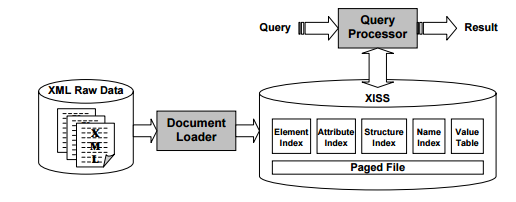
\includegraphics[width=1\textwidth]{img/Indexing}
    		\label{fig:xml-indexes}
    		\caption{Index in XML database~\cite{li2001indexing}}
	\end{figure}
\end{comment}
	\section{NoSQL Database}
	NoSQL databases(Not Only SQL) are distributed data management systems that store unstructured and semi-structured data. They are mainly known for its features like scalability, performance and availability~\citep{hecht2011nosql}.
	
	\textit{Scalability} is one of the key feature of NoSQL database system  where data instances are large and stored separately in different nodes. These databases are designed to store from terabytes to petabytes of data by trading-off its capacity to handle ACID properties to high scalability over a large number of nodes\cite{abramova2013nosql}. 	
	%\textit{Availability} 
   \par  Data in NoSQL is stored in commodity hardware in many servers, therefore network failures are common during data operation. If one or more nodes are unable to deliver the request of a client,  other nodes in the system can complete the operation without any loss. Data is replicated throughout the different nodes for fault tolerance.%System allows eventual consistency among the replicas of same the piece of data~\cite{nosql/comparision}
 %All the NoSQL databases are schema-less and they are read in a way that is tolerant to the changes.  
    \par 
NoSQL databases can be categorized into four categories based on the data model and design:
	\begin{itemize}
		\item 
			\textbf{Key/Value store}\\ The data representation of key/value stores are based on attribute pair, the data model expressed as collection of $<$$key$,$value$$>$ tuples. The key is unique and value can be varied. Since the values are uninterrupted arrays, keys are used to retrieve the stored data. They have very simple data structure and are schema free. Key/value stores are mostly used for simple operations, which are dependent on key attributes. The query operation on data can be uniquely performed by a key. The data can not be accessed or modified without a key. Some examples of key/value stores are DynamoDB, Riak,and Redis.
		\item 
			\textbf{Document-oriented databases} are based on semi-structured data model and unique key stores a value that has a tree like structure called \textit{document}. Attributes are key/value pair in JSON or in JSON like data format where data can be accessed by using key or specific value~\citep{hecht2011nosql}. Every document contains a special key "ID". Unlike in key/value stores, the values are not opaque and  they can be used to query the document. Document stores are schema free, so new attribute values can be added to the existing documents at any time. These documents are very convenient in schema migration tasks and data integration.  MongoDB, Couchbase, RethinkDB, and CouchDB are some example of this system.
		\item 
			\textbf{Column family databases} are also known as wide-column databases that store data table as a section of a column and each of the column can have  its own index structure. A graphical representation of column-family is given in  Figure~\ref{fig:column-family-2}. Column databases are suitable for heavy write and optimized for writing data to a smaller subset of records. It offer less flexibility than key stores as column families have to be predefined. Because of the tabular format, the graphical representation is similar to relational databases. Column family stores are more suitable for applications dealing with large amounts of data stored in the cluster, as it can be efficiently partitioned.  Cassandra, BigTable and HBase are categorized as wide column database.
		\item 
			\textbf{Graph databases} stores data as a  graph in the form of nodes and edges similar to a social network. These databases are efficient in handling heavily linked data. Data with many relationships are more suited for graph database as the operations like recursive joins can be replaced by efficient traversals. Neo4J and OrientDB are two example of this database.
	\end{itemize}
	
\begin{figure}[h]
	\centering
	\subfloat[column based database~\cite{wuoverview}]{
		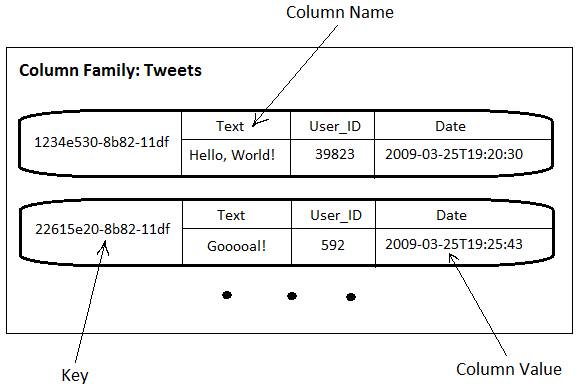
\includegraphics[width=.5\textwidth]{img/column-family}
		\label{fig:column-family-2}
	}
	\centering
	\subfloat[A document in document based database(JSON)]{
		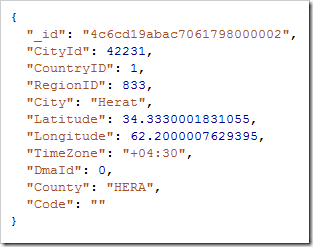
\includegraphics[width=.46\textwidth]{img/document-based-db}
		\label{fig:document-based-db}
	}
	\caption{column based database~\cite{wuoverview}}
	\label{fig:nosql-db-two}
	
\end{figure}

	\begin{figure}[h]
	\begin{lstlisting}[language=JSON,basicstyle=\scriptsize]
	{
		_id : "1"
		title : " MongoDB ",
		last_editor : "172.5.123.91" ,
		last_modified : new Date ("9/01/2015") ,
		body : " MongoDB is a..." ,
		categories : ["A", "B"] ,
		reviewed : false
	}
	\end{lstlisting} 
	\caption{}
	\label{sample-mongodb-document}
\end{figure}

	\subsection{MongoDB}\label{nosql-mongodb}
	%MongoDB is schema-free database system that manage data in the concept of database, collection and documents. A database contains one or more collections(can be compare to tables of RDBMS) which stores documents. Collections may contain any type of documents but generally they have documents with  similar schema. Data has flexible schema where collections do not enforce document to structure rather requirements of the application. Documents are modeled as a data structure following the JSON format which actually store as BSON, a binary variant of JSON, supports additional data types like ObjectId, timestamp, datetime etc.
	MongoDB is a schema-less document-oriented database developed by MongoDB Inc. with the support of Open Source community. 
\subsubsection{Data design} 
\paragraph{Document}
	A document is abstract and storable unit in MongoDB. It is the data structure expressed in the form of JSON and is stored in BSON, a binary variant of JSON that supports additional data types like ObjectId, timestamp, datetime etc. All the accessible data including database records, query selectors, index specifications, server configurations etc. are represented as documents. An example  MongoDB document is given in Figure~\ref{sample-mongodb-document}.
Every document is referenced with a unique key. A document is retrieved either by the key or any other attribute of the document. Collection in MongoDB is a group of documents and it is stored in a database. It is more convenient to group similar structured documents in a collection but not mandatory. MongoDB has two principles that allow the users to represent the relationships between the documents: \textit{references} and \textit{embedded} documents~\citep{mongodb:org}. 
\begin{itemize}
\item {Embedded:}\label{mongo:embedded}
    In Embedded document, data is nested. The documents are structured as sub-document in the form of Arrays or Objects~\citep{nosql/comparision}. 
    \item{Reference:}
    Unlike RDBMS, MongoDB has no support for joins, therefore related data is stored in a single document. In some cases, the related data can be stored in a separate collection. The relationship between data can be created by including links and references from one document to another as shown in Figure~\ref{fig:mongodb-ref-doc}.  The references between the data can be created in two ways:
\begin{itemize}
	\item {\textbf{Manual references}}
		In manual references, the application handles the relationship between documents by referencing \textit{\_id} field of one document to other. 
	\item \textbf{Database reference}(\textit{DBRefs})
	In  DBRefs reference, a first document's primary index field, collection name and optional database name of a document is used to reference to another document.
\end{itemize}



	% 	A document can be refer to another document with the help of collections of references.  where as referencing both collection name and database, MongoDB allows a document reference to multiple database.   With the reference of collection, a document can be reference to another document belonging different collection.
\end{itemize}

\begin{figure}[h]
	\centering
	\subfloat[Reference document]{
		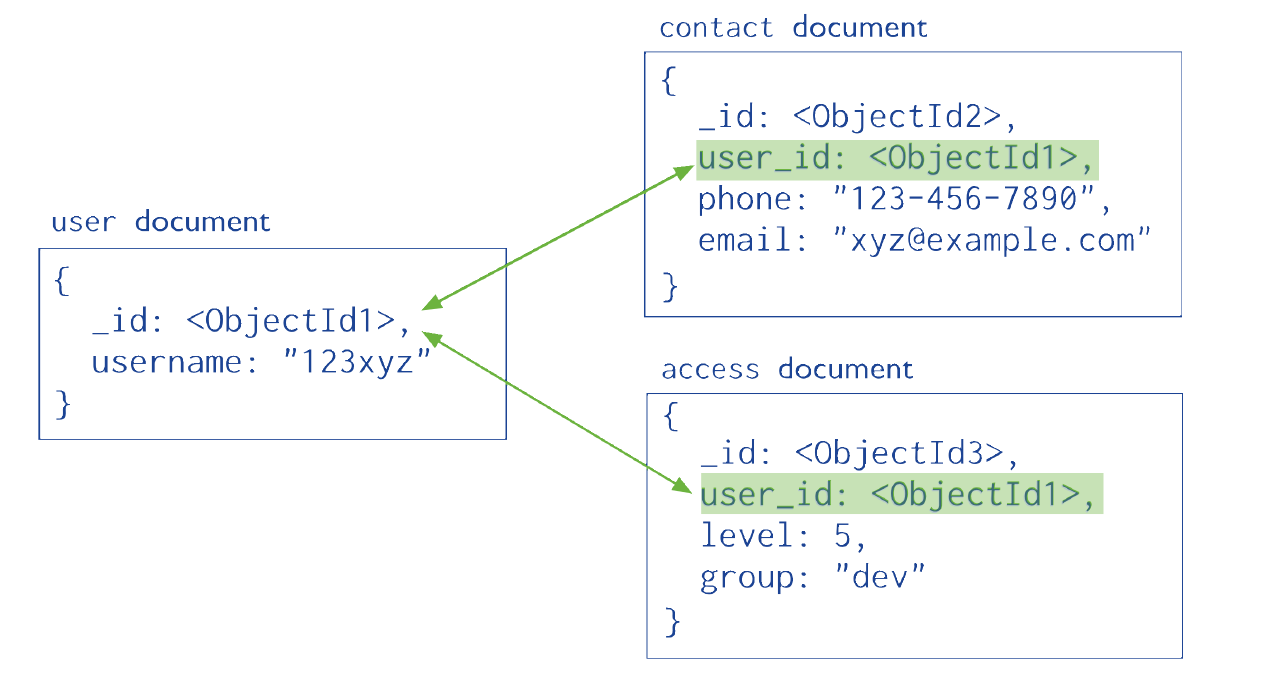
\includegraphics[width=.5\textwidth]{img/mongodb-reference}
		%{img/mongo/mongodb-reference}
		%\caption{R-tree structure}
		\label{fig:mongodb-ref-doc}
	}
	\centering
	\subfloat[Embedded document]{
		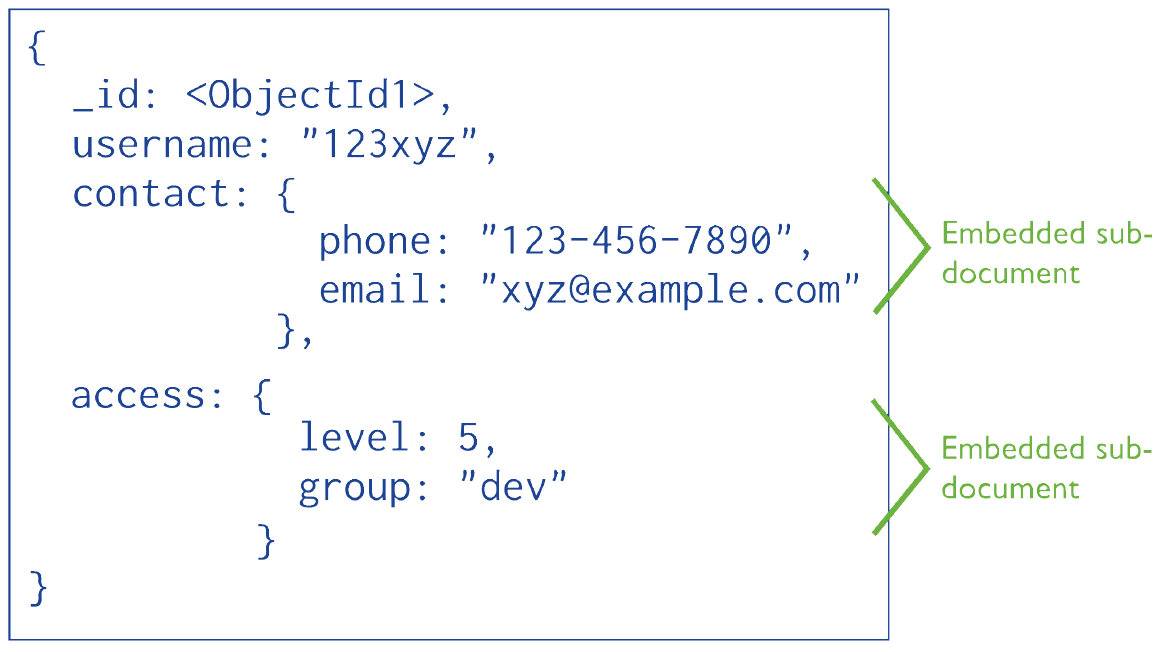
\includegraphics[width=.46\textwidth]{img/mongo/mongodb-embedded}
		%\caption{R-tree}
		\label{fig:mongodb-emb-doc}
	}
	\caption{MongoDB document structure~\citep{mongodb:org}}
	\label{fig:mongodb-doc}
	
\end{figure}

	\begin{figure}[h]
	\begin{lstlisting}[language=JSON,basicstyle=\scriptsize]
	{
		_id : "1"
		title : " MongoDB ",
		last_editor : "172.5.123.91" ,
		last_modified : new Date ("9/01/2015") ,
		body : " MongoDB is a..." ,
		categories : ["A", "B"] ,
		reviewed : false
	}
	\end{lstlisting} 
	\caption{MongoDB sample document}
	\label{sample-mongodb-document}
\end{figure}

\subsubsection{Indexing}\label{mong-xmark-indexing}

Each document in MongoDB is uniquely identified by a field \textit{\_id} which is also a primary index. Hence, the collection is sorted by \textit{\_id}~\citep{nosql/comparision}.
Apart from the primary index, MongoDB provides a mechanism to create secondary indexes for all fields of document. It supports various user defined indexes for field values including single field index, multikey index, multidimensional index, geo-spatial index, text index and hash index.
%Single field, multidimensional and multikey indexes are organized using B-tree, whereas geospatial index is implemented using quad trees.Once index is defined on a field,
\begin{itemize}
\item \textit{Single field index} only includes data from a single field of documents in a collection. 
\item \textit{Compound index} holds reference to the multiple fields within a collection's documents.
\item To index a field that contains an array value, MongoDB provides special indexing called \textit{Multikey index}.
\item \textit{Text index} helps efficient search of a string in documents.
\end{itemize}
\subsubsection{Query Model}\label{mongo-query-model}

%\todo{modify with christian's suggestions}
Queries in MongoDB are expressed in a JSON-like syntax and are sent to MongoDB as BSON objects by a database driver\citep{orend2010analysis}. A query can be specified by exact match on the embedded document or by using individual field with a \textit{dot notation}. It is used to access an element in document of an array or an object in the form of  $<$$array$.$index$$>$ or  $<$$object$.$childobject$$>$. For general queries, mongo shell can be used. It is an user friendly JavaScript shell that allows to implement callback functions to manipulate the data returned by the queries.  
\par
The Query model supports the following features:
\begin{enumerate}
	\item Queries over documents, embedded subdocuments and arrays
	\item Comparison operators
	\item Conditional Operators
	\item Logical Operators: AND and OR
	\item Sorting 
	\item Grouping
	\item Aggregation per query
\end{enumerate}

The \textit{find()} method is the most common way to retrieve data from a collection. It returns the subset of documents from specified collection with given criteria that are passed as parameters. If no any parameters is given, it returns everything from a collection.  The General syntax of find operation is given in Code~\ref{mongodb-find-sample}.
\begin{lstlisting}[language=JSON,caption=\textit{find} in MongoDB, label=mongodb-find-sample][H]
    db.collection.find(query, projection) 
\end{lstlisting}
 The \textit{query} specifies the criteria of document of a collection name \textit{collection}. The \textit{projection} selects of attributes of an documents to be return. For example, Code~\ref{mongodb-find-real} return the \textit{name} and \textit{age} from a collection  \textit{people} of country \textit{France} and \textit{age} is less than 5. 
\begin{lstlisting}[language=JSON,caption=\textit{find()} with query and project, label=mongodb-find-real][H]
    db.people.find({country:"France", age:{$lt:5}}, {_id:0, age:1, name:1}) 

\end{lstlisting}

\par
\paragraph{Aggregation Frameworks:}
 The \textit{find} method is not sufficient for the complex database queries like aggregation, grouping  and advanced data manipulation. MongoDB provides two frameworks for advanced query as well as parallel processing for the large collection:
 \begin{itemize}
		\item{ \textbf{Aggregation pipeline}} allows to execute series of operations using different operators like filtration, projection to produces desire result or performs aggregate operation.  It can be used for a single collection and uses  data operators like match, group, project, etc. in different stages. Every stage convert the documents as they pass through the pipeline. Data operators can be used  in any numbers of times.  The \textit{aggregate} function is responsible for this framework where it operates on a collection passing  entire documents into a pipeline. By using proper filtration operators like  skip, match and limit at the beginning  stage of the pipeline,  the frameworks can take advantages of existing indexes with processing scope limited to subset of documents, hence produces better performance in following stages~\cite{mongodbaggregation}. The aggregation pipeline has many limitations including data types, memory restriction to operators and output size~\cite{nosql/comparision}. Only 100 MB of RAM is assigned to pipeline stages. If this limit exceeds, the query will be broken. An option \textit{allowDiskUse} must be enable to write data to temporary files during staging.
		
				   \begin{lstlisting}[language=JSON,caption=An example Aggregation pipeline in MongoDB, label=mongodb-aggregation-pipeline, basicstyle = \scriptsize][h]
            db.open_auctions.aggregate([
                {$match:{reserve:{$exists:true}}},
		       {$project:{_id:0,reserve:{$multiply:["$reserve",2.20371]}}}
		       ]);
		  \end{lstlisting}
		  
		  \item{\textbf{MapReduce}} is a data processing framework design to support large volumes of data that goes beyond the limitations and restriction of aggregation pipeline.  In mapreduce,  \textit{map} function applies to each input document and emits the key-value pair as output. Any arbitrary sorting and limiting  of single collection is performed before map stage. The reduce applies to the map's output where a key is associated with multiple values to return the aggregated data. The output of \textit{reduce} may pass optionally through finalize function to further process the result. Mapreduce functions are written in JavaScript and executed in MongoDB's demon process ~\cite{mongodbaggregation}.  Unlike pipeline framework, Map-reduce support options for choosing to store result  data in a node as collection or return the output. Table~\ref{mongdb-mapreduce} illustrates a Mapreduce implementation in MongoDB. Two JavaScript function are defined for map and reduce. The \textit{runCommand} executes these functions in a collection.
		  
\end{itemize}		

\begin{longtable}{c|c}
\caption{Mapreduce in MongoDB}
 \label{mongdb-mapreduce}\\
	
	{\textit{map}} function(a) & {\textit{reduce}} function(b)\\
	\hline
	\begin{minipage}{.4\textwidth}
		\centering		
		\begin{lstlisting}[language=XML,basicstyle = \scriptsize,label=couchbase-map-sample]
map = function() {
           if(this.reserve){
            emit(this._id, this.reserve);
           }    
        };	
		\end{lstlisting}		
	\end{minipage} &
	\begin{minipage}{.49\textwidth}
		\centering
		\begin{lstlisting}[language=JSON, basicstyle =\scriptsize, label=couchbase-reduce-sample]
reduce = function(key,values) {
            return Array.sum(values);
        };
};
		\end{lstlisting}
	\end{minipage}
	\\
	\hline
	\multicolumn{2}{c}{
	    \scriptsize
	    
	Use: 	db.runCommand({"mapreduce" : 
	\textit{collectionName}, 
	                       "map" : \textit{map}, 
	                       "reduce" : \textit{reduce}})
		
	}
  	
  	\\
	\hline
	
\end{longtable}

%end here



\begin{comment}


\paragraph{System Architecture}
MongoDB can be run in two modes. In stand-alone mode, a single \textit{mongod} demon runs in a single node without any distribution and in shared mode various services are distributed to several nodes. 
\begin{figure}[h]
	\centering
	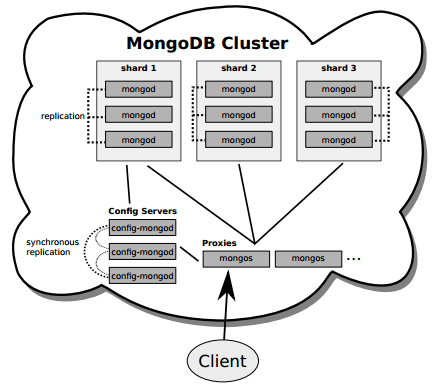
\includegraphics[width=0.5\textwidth]{img/mongo/clusters}
	%\caption{R-tree}
	\label{fig:mongodb-clusters}
\caption{MongoDB Clusters}
\end{figure} %reference




\end{comment}
	\subsection{Couchbase Server}\label{intro-couchbase}
	%Couchbase Server is NoSQL database that can be used both as a key-value store as well as document store system. As key-value store, it is able to store  multiple data type such as strings, numbers, datetime, and booleans as well as arbitrary binary data. The key-value generally treated as opaque Binary Large Object(BLOB) and don't try to parse it. For document store, data need to be store in the valid JSON format. Data in Couhbase Server are stored in logical unit called Buckets. These buckets can be technically compare as \texttt{database} in Mongodb or other RDBMS. All data type other than JSON can be retrieve only by their key. So it is important to check meta type of data stored in a single document before retrieval. Unlike MongoDB, Couchbase server Don't have concept of collections, so category of documents are identified by user defined type or group.
	 Couchbase Server is designed to be an operational data store for real-time data access. It is a NoSQL database that serves both as key-value and  document-oriented database. As a key-value store, it is able to store any type of data including  strings, numbers and binary data and the data is generally treated as an opaque Binary Large Object(BLOB) that do not try to parse it at the time of query. when being used as document store, data is stored in a valid JSON format. The data in Couchbase is stored in logical unit called buckets. These buckets  are isolated to each other and have their own RAM quota and replica settings. Buckets can be compared with \texttt{database} in Mongodb or other RDBMS. Couchbase recommends few numbers of buckets in a single cluster. A Bucket contains any type of data but data other than JSON, it can be retrieved only by its key. Therefore, it is important to check meta type of data that is stored in a single document before fetching. Each document is stored independently and there is not the notion of grouping documents like collections in MongoDB or tables in other RDBMS. The documents is separated by a user-defined type to distinguish the such documents.  For example, all the documents that are in \textit{user} and \textit{post} collections of MongoDB can be represented in Couchbase by adding a new field \textit{documentType}  in each document  with value \textit{user} and \textit{post} respectively.  
\label{cb-metadata}
\paragraph{Metadata}
For every value stored in a bucket, Couchbase Server generates following meta information that is associated with a document~\cite[p. 26]{cb/ostrovsky2014pro}. 
\begin{itemize}
	\item{Expiration}
		The Time to Live(TTL) also named as expiration time is the life time of the document. The default value of TTL is 0 that indicates document will never expire and also can be set as Unix epoch time after which document is removed.
	
	\item{Check-and-Set(CAS)}
		The CAS value is 64-bit integer that is updated by server when associated item is modified. It enables to update information only if unique identifier matches the identifier of the document that needed to be updated. CAS is used to manage concurrency when multiple client attempts to update the same document simultaneously. 
	\item{Flags} are 32 bit integer and are set of SDK specific use. For example, format in which data is serialize or data type of the object being stored.
\end{itemize}	
In addition of TTL, CAS and flags, three other meta information are stored at the time of document creation. The document's key \textit{id} is saved as part of metadata, \textit{type} is the type of a document either \textit{json} or Base64 encoded string for all other.
\paragraph{\textit{Document key}}
Every value in Couchbase Server is saved in unique key called document key. Unlike MongoDB, Couchbase  do not generate document key automatically and 250 characters string should be manually generated.
%In case of XMark data each \texttt{id} attributes of  \texttt{item}, \texttt{person}, \texttt{open\_auction}, \texttt{category} represent as key. In case of  \texttt{closed\_auction} and  \texttt{edge} key can be manually generated. 
\begin{figure}[h]
	\centering
	\subfloat[Views in Document Design]{
		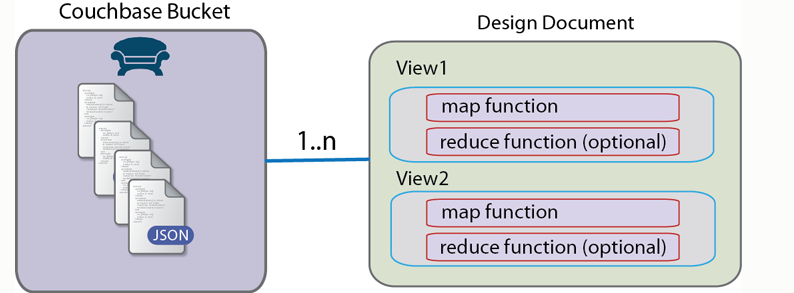
\includegraphics[width=0.4\textwidth]{img/cb/Small_view_elements}
		\label{fig:cb-views-design}
	}
	\centering
	\subfloat[View's Workflow]{
		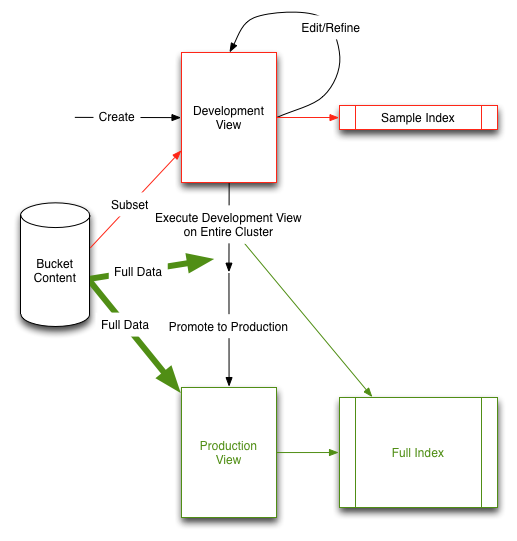
\includegraphics[width=0.4\textwidth]{img/cb/view-types-workflow}
		\label{fig:cb-views-workflow}
	}
	\caption{Couchbase Server's Document Design ~\citep{couchbasedocs}}
	\label{fig:cb-views-document-design}	
\end{figure}

\paragraph{Bucket and vBucket}
Couchbase Server uses data bucket as a logical container of information that provides a logical grouping of physical resources within a cluster~\citep{lichtenberg2013nosql}. Documents in Couchbase do not have their fixed schema and multiple documents  with different schema can be stored in same bucket. One or more attributes in documents are added to differentiate the various objects stored in a bucket and create indexes on them. Each bucket is split into 1024 logical partition called vBuckets. A vBucket is treated as a owner of subset of key where every key belongs to a vBucket~\ref{fig:cb-vbucket}.  
%%why we need vbucket

\begin{figure}[h]
	\centering
	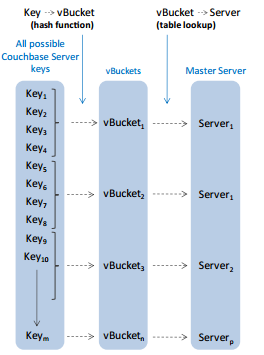
\includegraphics[width=0.4\textwidth]{img/vbucket2}
	\caption{ Couchbase  vBucket ~\cite{couchbasedocs}}
	\label{fig:cb-vbucket}
\end{figure}
%where is reference of images

\paragraph{Data Model}%repeat check once
A document is a basic unit of data manipulation in Couchbase  as a document store. All the documents are stored in JSON format without a predefined schema.

\paragraph{Querying and Indexing}
Query in Couchbase has to be done against pre-materialize views. The goal of view is to select the data, extract the attributes and information as client's need  and to produce the index on selected information. Views are defined in a specific kind of document called \textit{design document}~\ref{fig:cb-views-design}. These documents are bounded to a single bucket and cannot be executed from other bucket. The design document holds JavaScript code that implements \textit{Mapreduce} operations to create view's index in user defined format. The Mapreduce is achieved by two functions \textit{map} and reduce. Table~\ref{tbl:cb-mapreduce} illustrate a sample mapreduce function in Couchbase.

The \textit{map} function in design document identifies data from collection, process, filter them and output transformed values. Each document in a bucket is submitted to the \textit{map } function where document and metadata associated with the document are supplied as parameter to the \textit{map} function. After filtration, the \textit{emit} function in map returns the result as set of key/value pairs that are index. The output of map function can be zero or more "rows" according to the filter used in \textit{emit()} function. Each \textit{emit()} function returns a single row but can be called multiple times inside a single map function. The first parameter in \textit{emit} function is searchable text key and second parameter is the value.
The \textit{reduce} function is used to aggregate the numeric value generated in map phase. Couchbase has built-in reduce functions like \textit{\_count}, \textit{\_sum} and \textit{\_stats} aggregation. Table ~\ref{tbl:cb-mapreduce} illustrate an example of MapReduce  in Couchbase. The emit function at map phase returns the \textit{id} of document  as key and the price greater than 40 from documents that contains \textit{doctype} value "closed\_auctions". In \textit{reduce} phase, the the keys are grouped and values are counted.

%start here 
 In contrast to MongoDB,  Couchbase's queries are closely associated with client SDK where each operations has to perform through SDKs. On-demand query language  named "N1QL" is also in  progress of development but still stable version has to be released~\cite{couchbasen1ql}.


%end here from benchmarking sections.
\begin{table}[H]
\begin{longtable}{c|c}
	\caption{Mapreduce in Couchbase}
	\label{tbl:cb-mapreduce}\\
	\textit{map()} & \textit{reduce()}\\
	\hline
\begin{minipage}{.6\textwidth}
\begin{fakeJSON}[label=cb-mapreduce-map,basicstyle =\scriptsize]
function (doc, meta) {
   if(doc.doctype && doc.doctype=="closed_auctions"){
     if(doc.price){
       if(doc.price > 40) {
	      emit(doc.id,doc.price)
     	}
    }
  }
}

\end{fakeJSON}	
\end{minipage} &
\begin{minipage}{.2\textwidth}
\begin{fakeJSON}[label=cb-mapreduce-reduce]
	_count
\end{fakeJSON}
\end{minipage}\\
\end{longtable}
\end{table}


	
	\subsection{RethinkDB}
	%RethinkDB is distributed database system to store  JSON documents that uses efficient query languages named ReQL which automatically parallelize queries in multiple machines. RethinkDB has similar concept of store database like MongoDB. A database contains schema-less table, where documents are stored in the form of JSON. Unlike MongoDB, RethinkDB query language supports join queries between tables.
	RethinkDB is an open-source distributed document-oriented database system to store JSON documents. One of the unique feature of RethinkDB is the changefeed by the server to the client. 
Instead of a client request, the changes in database is streamed to the client application in realtime. In case of multi-users environment, any database  update is automatically notified.
\par
ReQL is the query language  of RethinkDB and it is based on three main principles:
 \begin{itemize}
 \item  It is  embedded  as programming language. Queries are constructed by making function call. 
 \item ReQL queries are chainable that can be passed as pipeline from one stage to another. Complex operation can be performed using series of simple queries together by using dot operators (\.) . 
 \item All the queries are executed in server without any intermediate network round trip between the server and clients.
 \end{itemize}
  
\subsubsection{Data Model}
There are two ways to model relationships between the documents: 
\begin{itemize}
	\item \textbf{Embedded arrays:} In this method, the related sub-documents are inserted with a specific key inside a document as in MongoDB ~\ref{mongo:embedded}. The advantages of using embedded arrays are:
		\begin{itemize}
			\item The Queries tend to be simpler. 
			\item If a dataset  does not fit into RAM, then the data is loaded  from the disk and it is faster compared to tables. 
		\end{itemize}
		Disadvantages of embedded arrays are: 
		\begin{itemize}
			\item Before any operation, data should be loaded into memory. In case of any updates, the document will rewrite the full array to the disk.
		\end{itemize}
		
	\item 
	\textbf{Multiple Table Approach:} In this approach, documents with similar structures are stored in multiple tables similar to collection in MongoDB. These tables are connected by reference key. Unlike embedded arrays, operation of a table does not required to load data from reference table in memory.
\end{itemize}

\subsubsection{Query Model}
RethinkDB's query language ReQL is embedded as programming language and JavaScript expressions can be used anywhere as a part of the query. The anonymous function, also known as lamda function, is a part of the query language that gives more flexibility for retrieving data. All the ReQL queries are chainable therefore, the dot \{.\} operator at any point of query can be extended to multiple levels as shown in Code~\ref{reql-chainable}.
	\begin{lstlisting}[language=JSON,caption=Chainable Query in ReQL, label=reql-chainable, xleftmargin=-40pt, 	basicstyle=\ttfamily\footnotesize][h]
		r.table("users").run(conn)
		r.table("users").pluck("last_name").run(conn)
		r.table("users").pluck("last_name").distinct().run(conn)
		r.table("users").pluck("last_name").distinct().count().run(conn)
	\end{lstlisting} 
The queries are built up on client side and send to the server when the \textit{run()} is called. Then the server automatically parallelized the queries into different nodes. whenever possible, the query execution is splitted into different cluster and data-centers.
\par
Unlike other NoSQL databases, RethinkDB supports join queries between the tables in one-to-many or many-to-many relationships in distributed manner. 
%start here from bechmarking section
%there should be some changes
\subsubsection{Indexing}
	RethinkDB uses B-trees to store indexes. When tables are created, there is an option to specify the attribute as a primary key. \textit{id} behaves as a primary key if the attribute is not specified and it is used to index the document. If there is no  primary key, a random unique string is automatically generated to index the document. Beside the primary index, RethinkDB supports simple, compound, secondary, geospatial indexes. Beside that any arbitrary expression can be used to create index from any type of user defined expressions like lamda functions. Every query including update operations uses only one index.
	 Only \textit{getAll()} \textit{between()}, \textit{eqJoin()} and \textit{orderBy} functions can use secondary index.		
	%\subsection{Summary}
	%All document oriented NoSQL database store data in the form of JSON or JSON like format and XML is the basic unit of storage for XML database. for data migration, it is necessary to understand the properties of XML and JSON Data format.	
	\chapter{Semi-structured Data: XML and JSON}\label{semi-structure-data}
		XML is a textual markup language in which data elements are ordered by nature: \textit{string} is the core data type, other data types like integers, floats, user-defined abstract data, etc. are derived. ~\citep{xmark/original}. It is both human and machine readable, and  used as the data exchange format in the web. XML is derived from Standard Generalized Markup Language(SGML) and standardized by the World wide web Consortium(W3C).
\par
%JSON is a programming language model that consist of minimal textual representation and a subset of JavaScript. its web services. As it is the subset of JavaScript, it is perfectly suited 
    JSON is another data format that is designed to exchange the data in key/value format. As subset of JavaScript, it perfectly suits for the web-based services. In modern browsers parsing JSON is comparatively much faster than XML. A JSON document consists of two data structures:
\begin{itemize}
	\item Object, an unordered collection of key/value pair that are encapsulated with curly braces \{ and \}. The key is a string embedded in double quotes and followed by a column(:) to its value. The key must be unique for each object.
	%TODO:   which are numbers of key value pairs
	\item Arrays, that are an ordered list of values
\end{itemize}
A JSON value can be Object, Array, number, string, true, false and null.
  %XML is suitable for document description, that is the hierarichal elements can also have attributes, which is not available in JSON. JSON is much preferred for text format object serialization, because of its concise syntax for defining the lists of elements. An additional library is required for XML to work with JavaScript. Whereas JSON can directly parse and work directly with js objects.
  
\section{Problem to translate from XML to JSON}
JSON and XML are conceptually similar as they both are text based markups, that are designed to represent data in human-readable form, exchangeable across multiple platforms and parsable by common programming language, but differ in their syntax~\citep{lee2011jxon}. JSON and XML are fundamentally incompatible with each other, as listed below:
\begin{itemize}
\item \textit{Root node and anonymous values}
\\
Each XML document has one root node. JSON supports anonymous values also referred as string values, that do not need key/value pairs. For example, in Table~\ref{tbl:Anonymous-xmljson} the XML root node is implicitly created in the model and will not have a textual representation in JSON.

	\item \textit{Arrays}\\
		Arrays are native data types of JSON that does not exists in XML. There is no direct markup for arrays in XML.
		\item \textit{Identifiers}\\
		XML is much more restrictive for identifiers compared to JSON, which allows any string to be an identifier. Translating from XML to JSON does not cause any problem, but in reverse case it might lead to not well formed XML. For example, "Hello World" is a valid identifier in JSON but not valid attribute or element in XML, as there is a whitespace between the two words.
		\item \textit{Attributes}\\
		JSON does not have the notion or any representation of attributes. When mapping data from XML to JSON, the attributes are translated to name object members along with other child elements. This information will be lost in mapping from JSON to XML.
		\item \textit{Namespaces}\\
		XML supports namespaces to identify  unique element and attributes in a document. Namespaces do not exist in JSON. Mapping QNames in XML with namespaces to JSON can lead to ambiguous and duplicate names.
		%\item \textit{Others}\\
		%TODO: {Processing Instructions, Character Set, Comments, Encodings}
		%There are also some other problems like processing instructions and  comments which XML supports but not in JSON. Other issues for example, character set and encoding are not easily exchangeable in both format.
\end{itemize}

\begin{longtable}{c|c}
	\caption{Anonymous values of JSON in XML}
	\label{tbl:Anonymous-xmljson}\\
	\textbf{JSON} & \textbf{XML}\\
	\hline
\begin{minipage}{.35\textwidth}
\begin{fakeJSON}[basicstyle=\scriptsize]
	["Hello World"]
\end{fakeJSON}	
\end{minipage} &
\begin{minipage}{.45\textwidth}
\begin{fakeXML}[label=xml-anonymous]
	<root>Hello World</root>
\end{fakeXML}
or
\begin{fakeXML}
	<root value="Hello World">
\end{fakeXML}
\end{minipage}\\
\end{longtable}
	
	
		
\section{Mapping}
XML and JSON have different data types. XML has more flexible data types compare with JSON. Table~\ref{tbl:xml-json:types} types of data are listed for simple XML and relevant JSON types.
\begin{longtable}[hbtp]{c|c}
\caption{Translation of simple XML data types into JSON}
\label{tbl:xml-json:types}\\

\textbf{XML type definition} & \textbf{JSON type definition}\\
\hline

\begin{minipage}{.4\textwidth}
  \begin{lstlisting}
xs:string
  \end{lstlisting}
\end{minipage} &
\begin{minipage}{.4\textwidth}
\begin{lstlisting}
{
  "type": "string"
}
\end{lstlisting}
\end{minipage}\\

\hline
\begin{minipage}{.4\textwidth}
  \begin{lstlisting}
xs:boolean
  \end{lstlisting}
\end{minipage} &
\begin{minipage}{.4\textwidth}
\begin{lstlisting}
{
  "type": "boolean"
}
\end{lstlisting}
\end{minipage}\\

\hline
\begin{minipage}{.4\textwidth}
  \begin{lstlisting}
xs:float
xs:double
xs:decimal
xs:integer
(All Other Numbers)
  \end{lstlisting}
\end{minipage} &
\begin{minipage}{.4\textwidth}
\begin{lstlisting}
{
  "type": "number"
}
\end{lstlisting}
\end{minipage}\\
\hline

\begin{minipage}{.4\textwidth}
	\begin{lstlisting}
	xs:anySimpleType
	(Remaining all others)
	\end{lstlisting}
\end{minipage} &
\begin{minipage}{.4\textwidth}
\begin{lstlisting}
{
	"type": "string"
}
\end{lstlisting}
\end{minipage}\\
\end{longtable}


For complex type elements in XML that contains nested elements and attributes, JSON can have two possibilities: either an object or an array type.  Sectio~\ref{xml-to-json-migration} illustrates the translation of complex XML type to JSON.

\section{Migration from XML to JSON}\label{xml-to-json-migration}
We have defined the several stages to convert XML to JSON documents:
\begin{enumerate}[label=\textbf{Step \arabic *.}]
	\item~\\
	\textbf{XML to JSON friendly XML}
	\par
	Algorithm~\ref{algorithm-JSONXML} provides pseudo-code for XML-to-JSON friendly XML. At the first step of the conversion process, all attributes of XML document are represented as ordered child elements. There can be more than one attribute that is inserted in order. Then, the inserted attributes are deleted.  XML nodes can contain both text and element node as a child, whereas JSON can have only key/value pair or value only for array. Each text node that  has also an element node as sibling is moved to \textit{childtext}(name of the element) node. At the end of the first step, if an element contains another element as a child node, then it is represented as object type of JSON. It is necessary to identify if a siblings of an element node($S$) has same the element name or not. If this condition exists, $S$ is represented as an array in JSON. All the child nodes of all siblings are moved inside $S$ node. If $S$ is already  object type  then it is replace with array type  a new array is added. %In this algorithm, the loop of one action affect other, so they are looped independently.
	
	\item~\\
	\textbf{Data type of XML-to-JSON data type}
	\par
	After JSON-friendly XML in Step 1, the complex data type of XML is marked as either object or array type of JSON illustrated in Table~\ref{tbl:xmljson}. In this Step,  as in 
	Algorithm~\ref{algorithm-JSONXML-type}, all the scalar type of XML document are identified and marked with their type in JSON according to Table ~\ref{tbl:xml-json:types}.
	\item~\\
	\textbf{Mapping XML to JSON object or array}
	\par
	After Step 1 and 2, a complete JSON-friendly XML is generated. All XML objects and arrays are mapped to $<$$key$, $value$$>$ pair of JSON and their respective data types. Table ~\ref{tbl:xmljson-convert-3} illustrates final conversion from XML to JSON.
\end{enumerate}

		\begin{algorithm}[h]
			\DontPrintSemicolon
        	\begin{algorithmic}
        	\STATE Initialize $D = "{XML} document"$;
        	  	\FORALL{descendant-or-self node of  $D$,  $X$ which has attributes $A$  }
        			\STATE move  all attributes  $A$ to ordered child element of $X$\;
        		\ENDFOR
        		
        		\FORALL{descendant-or-self node of  $D$,$X$ }
        			\IF{ $X$ contains Text node and element node Both}
        				\STATE create new element "childtext" \;
        				\STATE move text node to "childtext" element \;
        			\ENDIF
        		\ENDFOR
        		
        		\FORALL{descendant node of  $D$,$X$ }
        			\FORALL{child element $C$ in $X$}
        				\IF{ $C$ has siblings $S$ with same \textit{name} }
        					\STATE convert $C$ as Array type\;
        					\STATE move child of $S$ into $C$ as $<$\_$>$ element\;
        				\ENDIF
        				\IF{ $C$ has child element }
        					\STATE convert $C$ as Object type\;
        				\ENDIF
        			\ENDFOR
        		\ENDFOR
        	\end{algorithmic}
        	\caption{Pseudocode to convert normal  XML to JSON friendly XML}\label{algorithm-JSONXML}
\end{algorithm}
	
 \begin{algorithm}[h]
			\DontPrintSemicolon
        	\begin{algorithmic}
        	\STATE Initialize $D = "{XML} document"$;
        	  	\FORALL{descendant-or-self node of  $D$ as $C$}
        			\IF{ $C$ has no attribute "type" }
        				\STATE get content of $C$ \;
                        \STATE identify content type according to Table ~\ref{tbl:xml-json:types}. and add attribute to $C$ "type" \;
        			\ENDIF
        		\ENDFOR
        	\end{algorithmic}
        	\caption{ convert data type of XML to JSON data type(Step 2)}\label{algorithm-JSONXML-type}
        \end{algorithm}

\begin{longtable}{c|c}
	\caption{XML to JSON friendly XML(step 1)}
	\label{tbl:xmljson}\\
	\textbf{XML} & \textbf{ Algorithm~\ref{algorithm-JSONXML} }\\
	\hline
\begin{minipage}{.4\textwidth}
\begin{fakeXML}
<info>
  <name>
    <f>a</f>
  </name>
  <age>24</age>
  <ismarried>false</ismarried>
  <city name="Armonk"/>
  <state>NY</state>
  <contact>
	 home
    <p>993-330</p>
    <p>993-331</p>
  </contact>
</info>
\end{fakeXML}	
\end{minipage} &
\begin{minipage}{.55\textwidth}
\begin{fakeXML}
<info type="object">
  <name type="object">
    <f>a</f>
  </name>
  <age>24</age>
  <ismarried>false</ismarried>
  <city type="object">
    <name>Armonk</name>
  </city>
  <state>NY</state>
  <contact type="object">
	<childtext>home</childtext>
    <p  type="array" >
	   <_>993330</_>
	   <_>993-331</_>
    </p>
  </contact>
</info>
\end{fakeXML}
\end{minipage}\\
\end{longtable}

\begin{longtable}{c|c}
	\caption{XML to JSON friendly XML(step 2)}
	\label{tbl:xmljson-2}\\
	\textbf{Algorithm~\ref{algorithm-JSONXML}} & \textbf{ Algorithm~\ref{algorithm-JSONXML-type} }\\
	\hline
\begin{minipage}{.4\textwidth}
\begin{fakeXML}
<info type="object">
  <name type="object">
    <f>a</f>
  </name>
  <age>24</age>
  <ismarried>false</ismarried>
  <city type="object">
    <name>Armonk</name>
  </city>
  <state>NY</state>
  <contact type="object">
	 <childtext>home</childtext>
    <p  type="array" >
	   <_>993330</_>
	   <_>993-331</_>
    </p>
  </contact>
</info>
\end{fakeXML}	
\end{minipage} &
\begin{minipage}{.55\textwidth}
\begin{fakeXML}
<info type="object">
  <name type="object">
    <f type="string">a</f>
  </name>
  <age type="number">24</age>
  <ismarried type="boolean">false</ismarried>
  <city type="object">
    <name type="string">Armonk</name>
  </city>
  <state>NY</state>
  <contact type="object">
	 <childtext type="string">home</childtext>
    <p  type="array" >
	   <_ type="number">993330</_>
	   <_ type="string">993-331</_>
    </p>
  </contact>
</info>
\end{fakeXML}
\end{minipage}\\
\end{longtable}

	\begin{longtable}{c|c}
	\caption{XML to JSON (step 3.)}
	\label{tbl:xmljson-convert-3}\\
	\textbf{XML(After step 2)} & \textbf{JSON}\\
	\hline
\begin{minipage}{.55\textwidth}
\begin{fakeXML}
<info type="object">
  <name type="object">
    <f type="string">a</f>
  </name>
  <age type="number">24</age>
  <ismarried type="boolean">false</ismarried>
  <city type="object">
    <name type="string">Armonk</name>
  </city>
  <state type="string">NY</state>
  <contact type="object">
	<childtext type="string">home</childtext>
    <p  type="array" >
	   <_ type="number">993330</_>
	   <_ type="string">993-331</_>
    </p>
  </contact>
</info>
\end{fakeXML}	
\end{minipage} &
\begin{minipage}{.5\textwidth}
\begin{fakeJSON}
{
    "info":{
      "name":{
        "f":"a"
      },
      "age":24,
      "ismarried":false,
      "city":{
        "name":"Armonk"
      },
      "state":"NY",
      "contact":{
	   "childtext":"home",
        "p":[
          993330,
          "993-331"
        ]
      }
    }
}
\end{fakeJSON}
\end{minipage}\\
\end{longtable}
	
\section{XMark}\label{xmark}
			The XML benchmarking project XMARK~\citep{xmark/original} is one of the most popular and commonly used XML benchmarking projects to date. It provides a small executable tool called \textit{xmlgen} that can be used to create a synthetic XML dataset based on a fixed schema describing an Internet auctions database. xmlgen can be used to build a single record with a large, hierarchical XML tree structure. A factor is specified to scale the generated data, ranging from a few kilobytes to an arbitrary size, limited by the capacity of the system. The textual part of the resulting XML document is constructed from 17,000 most frequently occurring words of Shakespeare's plays.

\subsection{Dataset}\label{xmark-dataset}
The main entities of XMark data are in two groups. The first group consists of  \textit{person}, \textit{open\_auction}, \textit{closed\_auction}, \textit{item} and \textit{category}. The second group's entities \textit{annotation} and \textit{description} are natural language text and document-centric element structure. The relationship between the entities in the first group are expressed as reference and the second group entities are embedded into subtree of first group entities. Figure~\ref{fig:xmark-tree} shows the XMark dataset with the following properties:
\label{xmark:desc:each}
\begin{itemize}	
	\item
	\textit{people} is a collection of \textit{person} element that is connected to buyer and seller of \textit{open\_auctions}, \textit{closed\_auctions}, etc. Each person has an unique identifier \textit{id} to reference to another entities like open\_auctions and closed\_auctions.
	\item
	\textit{regions} is a collection world regions \textit{africa}, \textit{asia}, \textit{australia}, \textit{europe}, \textit{namerica} and \textit{samerica}. Each of these region has \textit{item} elements which are the objects for sale or already sold. Each \textit{item} carries a unique identifier \textit{id} and has properties like name, payment information, description and a reference to the seller that are encoded as elements. 
	\item
		\textit{open\_auctions} refers to current auctions that contains bid history(increase/decrease over time) with references to bidders and sellers, current bid, the time interval of bid accepted, the status of the transaction, a reference to the item being sold etc.
	\item
		\textit{closed\_auctions} contains auctions that are successfully completed. They have properties like buyer and seller information reference to \textit{person}, a reference to sold items, amount of price, quantity of sold items, date of transaction, type of transaction, and much more.
	\item 
		\textit{categories} is used to classify the items. Each category has a unique identifier used to reference an item, a name and a description.
	\item
		  A \textit{catgraph} links categories into a network.  The full semantics of the XMark dataset can be found in~\cite{xmark/original}.
\end{itemize}
The full ER-Diagram of XMark dataset is illustrated in Fig.~\ref{fig:xmark-schema}. 
\begin{figure}[H]
	\centering
	\subfloat[Reference in \textit{XMark}]{
		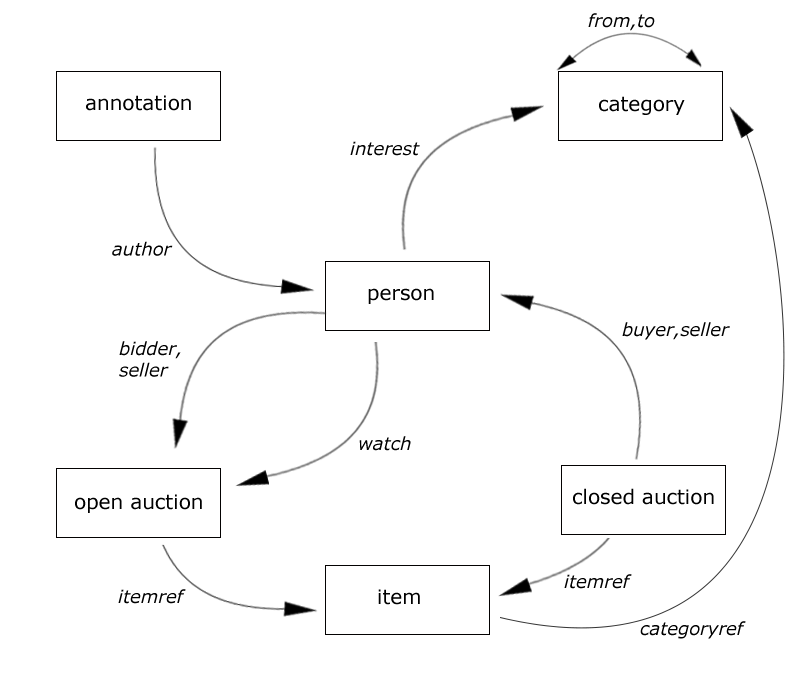
\includegraphics[width=0.40\textwidth]{img/xmark/101}{ %xmark-references.png
			\label{fig:xmark-reference}
		}
	}
	\centering
	\subfloat[Reference in \textit{XMark} dataset tree]{
		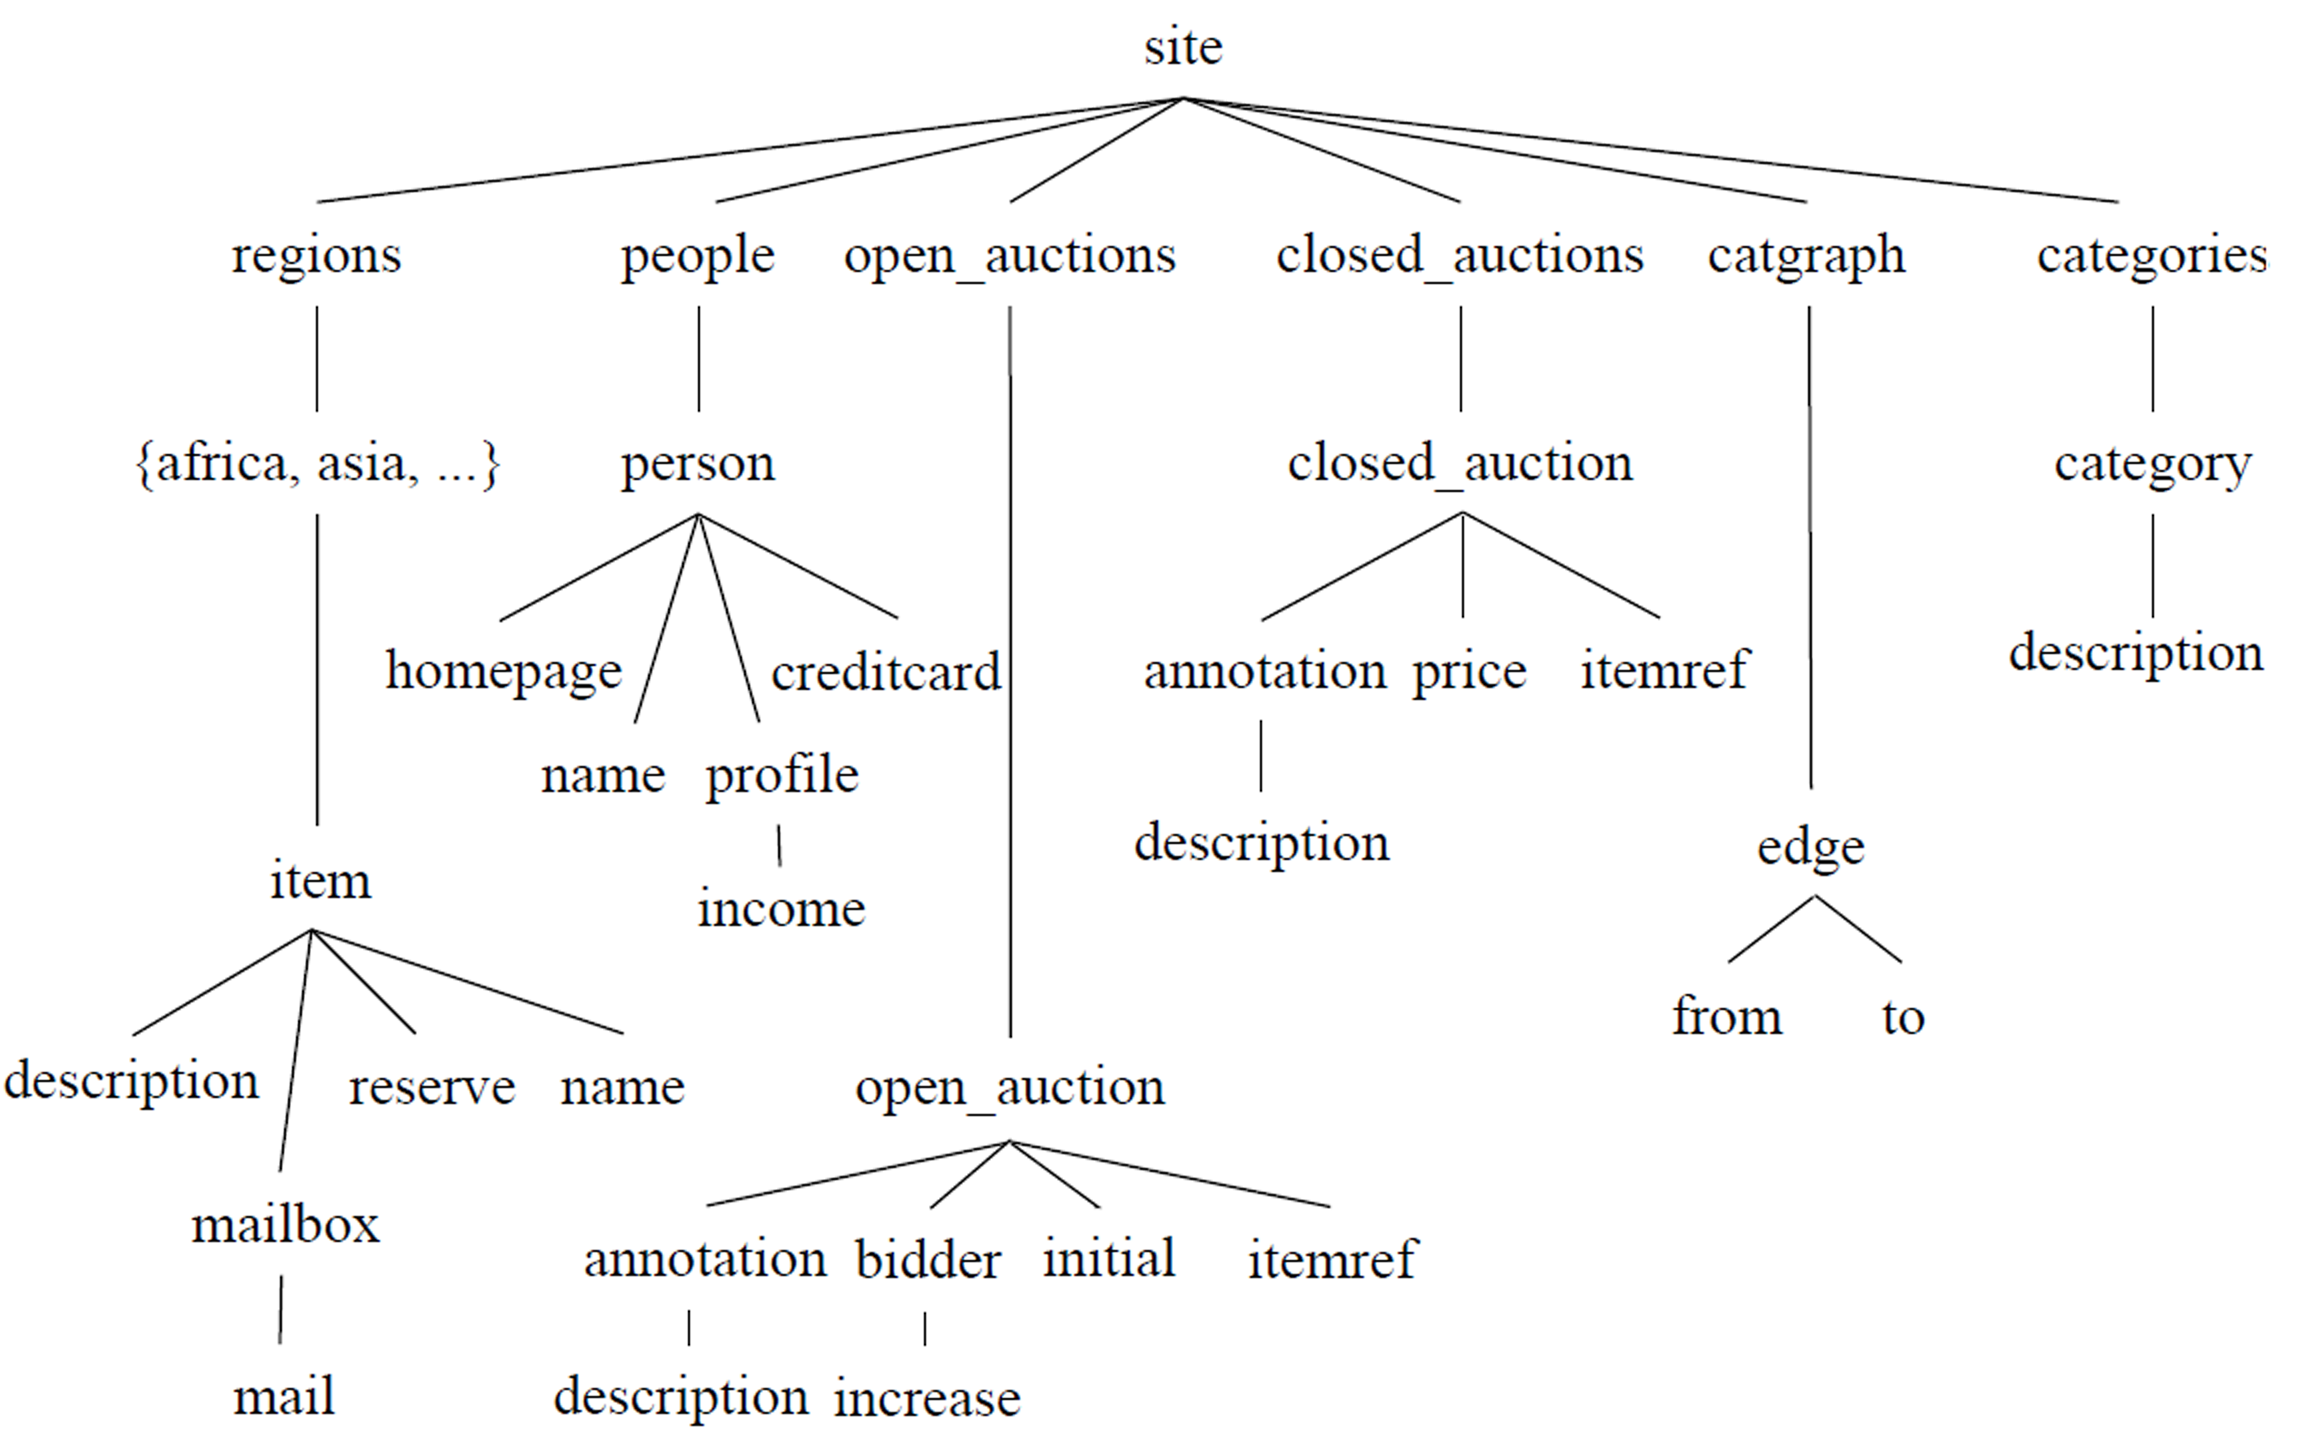
\includegraphics[width=0.4\textwidth]{img/xmark-tree.png}{
			\label{fig:xmark-tree}
		}
	}
	\caption{XMark data tree and reference~\citep{xmark/original}}
	\label{fig:xmark-tree-reference}
\end{figure}
\begin{figure}[H]
	\centering
	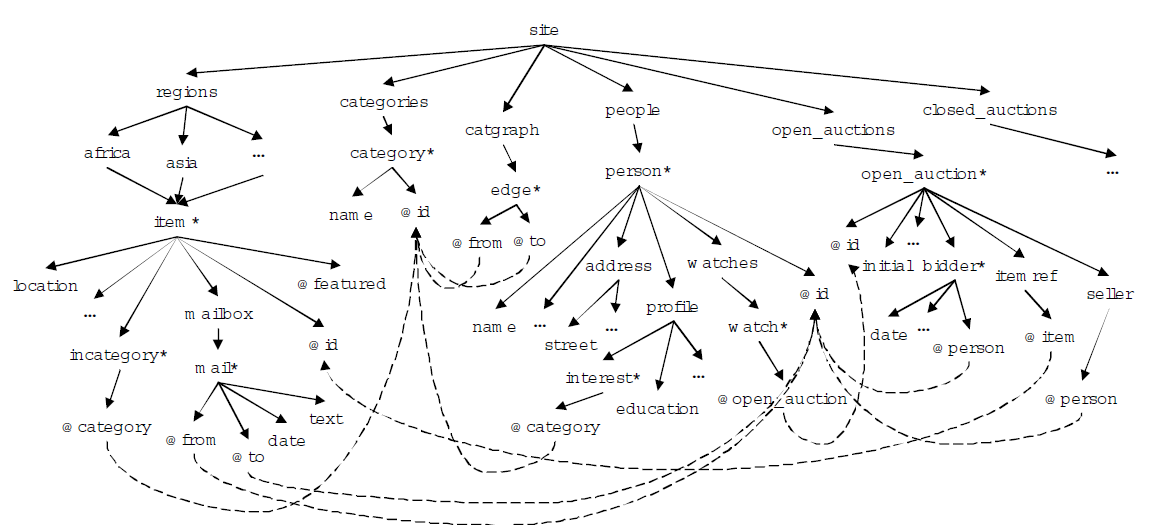
\includegraphics[width=0.90\textwidth]{img/xmark-schema-4}
	\caption{XMark ER-Diagram. Nodes, solid arrows, and dashed arrows represent schema elements (or attributes, with prefix '@'), structural links, and value links, respectively. Elements with suffix '*' are of SetOf type\citep{xmark/schema-sumerize}}
	\label{fig:xmark-schema}
\end{figure}

\subsection{XMark Queries}\label{xmark-queries}
The XMark project contains XQuery queries that focuses on the various aspect of language such as aggregation, reference, ordering, wildcard expressions, joins, user defined functions, etc.\citep{xmark/mlynkova2008xml}.The textual representation of 20 different XQuery expressions is reprinted in  Table~\ref{tab:xmark-queries}. These queries are divided into different categories  based on the  multiple functionalities of XQuery: 
\begin{enumerate}[label=\arabic*.]
\item  First category tests execution of exact match of string in specified path and consists of only query Q1.
\item It  helps to analyze order access of an XML document. Query Q2, Q3 and Q4 are grouped here.
\item  Query Q5 is evaluates the casting of a value.
\item Queries Q6 and Q7  evaluate regular path expressions.

\item This category investigates the referencing of a document to another and consists of query Q8 and Q9

\item Query Q10 reconstructs a complex results from the result of a query

\item Two queries, Q11 and Q12 are join query based on values.  The difference between this category's queries and reference queries Q8 and Q9 is that references are specified in DTD and may optimize with object identifiers whereas Q11 and Q12 are have join on the basis of values.

\item Query Q13  benchmarks the portion reconstruction of original XML document.

\item In this category the full text search  using single word is implemented. Q14 is in this category

\item The purpose of queries 15 and 16 is to observe the path traversals without using wildcards.

\item Query Q17 tests the ability to deal with missing values

\item This category deals with user defined functions and contains query Q18

\item The query Q19 is use to evaluate Sorting.

\item The last category observe the aggregation with the help of query 20.

\end{enumerate}

\begin {table}[htpb] 
\centering
\caption {The XMark queries. Source:\citep{xmark/original}}
\label {tab:xmark-queries}
\begin{tabular}{r|l}
	\hline
	Q1&Return the name of the person with ID 'person0'.\\
	\hline
	Q2&Return the initial increase of all open auctions.\\
	\hline
	Q3&Return the first and current increase of all open auctions whose current\\
	&increase is at least twice as high as the initial increase.\\
	\hline
	Q4&List the reserves of those open auctions where a certain person issued\\
	&a bid before another person.\\
	\hline
	Q5&How many sold items cost more than 40.\\
	\hline
	Q6&How many items are listed on all continents?\\
	\hline
	Q7&How many pieces of prose are in our database?\\
	\hline
	Q8&List the names of persons and the number of items they bought.\\
	&(Joins person, closed\_auction)\\
	\hline
	Q9&List the names of persons and the names of items they bought in Europe.\\
	&(Joins person\_auction, item)\\
	\hline
	Q10&List all persons according to their interest; use French markup\\
	&in the result.\\
	\hline
	Q11&For each person, list the number of items currently on sale whose\\
	&price does not exceed 0.02\% of the person's income.\\
	\hline
	Q12&For each richer-than-average person, list the number of items currently\\
	&on sale whose price does not exceed 0.02\% of the person's income.\\
	\hline
	Q13&List the names of items registered in Australia along with\\
	&their description.\\
	\hline
	Q14&Return the names of all items whose description contains the word 'gold'.\\
	\hline
	Q15&Print the keywords in emphasis in annotations of closed auctions.\\
	\hline
	Q16&Return the IDs of those auctions that have one or more keywords\\
	&in emphasis.\\
	\hline
	Q17&Which persons don't have a homepage?\\
	\hline
	Q18&Convert the currency of the reserve of all open auctions to\\
	&another currency.\\
	\hline
	Q19&Give an alphabetically ordered list of all items along with their location.\\
	\hline
	Q20&Group customers by their income and output the cardinality of each\\
	&group.\\
	\hline
\end{tabular}
\end {table}

		\subsection{XMark data into NoSQL database}\label{xmark-nosql}
			A synthetic XMARK dataset consists of a huge record in tree structure~\citep{xmark/VIST}. As mentioned in Section~\ref{xmark-dataset}, each subtree, \textit{regions}, \textit{people}, \textit{open\_auctions}, \textit{closed\_auctions}, \textit{catgraph} and \textit{categories} contain large numbers of instances that are indexed during database creation. At first, in most NoSQL database, the dataset cannot be a huge block but in fragmented form with each instances having it's own index structure. Besides this, NoSQL databases limits the size of a single document. For example, MongoDB has a limitation of 16 MB per document, the maximum size of documents allowed in RethinkDB is 64 MB and Couchbase Server can have value of a key upto 20 MB. The data model of NoSQL does not match single instance model of XML database.
\par 
To model XMark dataset into NoSQL, we have broken down the tree structure of XMark into set of sub-structure without losing the overall data. Each NoSQL database has their own data model, hence it is required to define a model for each of those databases separately.

The generalized concept of  XMark data into NoSQL databases is explained here but it might slightly differ from one another. 

All sub-trees \textit{regions}, \textit{people}, \textit{open\_auctions}, \textit{closed\_auctions}, \textit{catgraph} and \textit{categories} are the basic unit for the document fragmentation. Each of these sub-trees stores entities \textit{item}, \textit{person}, \textit{open\_auction}, \textit{closed\_auction} and \textit{category} respectively as mentioned in Section~\ref{xmark-dataset}. These entities represent the documents in NoSQL databases. In each document, one special field \textit{doctype} is added to represent the name of parent sub-tree. For example, in case of \textit{people} sub-tree, the value of \textit{doctype} is \textit{people}. This key/value set will be the part of a document as  given in Table~\ref{tbl:xmark-xml-json}(b). The \textit{doctype} has all-together six distinct values : \textit{categories}, \textit{catgraph}, \textit{people}, \textit{open\_auctions} and \textit{closed\_auctions}. There is an exceptional case for \textit{item} entities. It has \textit{regions} as grandparent and name of different regions like \textit{asia}, \textit{europe}, \textit{australia}, \textit{namerica}, \textit{samerica} etc. as the parent.  The \textit{doctype} for \textit{item} document will be \textit{regions} as other. To represent the name of regions like \textit{asia}, \textit{europe}, etc.,  one field with key \textit{regions} is added in each document. 
Table~\ref{tbl:xmark-item-type} illustrate the extra attribute added in each of document.

\begin{longtable}{c|c}
	\caption{ Extra attribute of a document in NoSQL}
	\label{tbl:xmark-item-type}\\
    {for \textit{person} and all other entities except \textit{item} } & {for \textit{item} which has region name \textit{asia}}\\
	\hline
\begin{minipage}{.4\textwidth}
\begin{lstlisting}[language=JSON]
{
	"doctype":"people"
}
\end{lstlisting}
\end{minipage} &
\begin{minipage}{.4\textwidth}
\begin{lstlisting}[language=JSON]
{
	"doctype":"regions",
	"regions":"asia"
}
\end{lstlisting}
\end{minipage}
\end{longtable}

A sample document of NoSQL database along with respective XMark document is illustrated in  Table~\ref{tbl:xmark-xml-json}. The conversion from XML to JSON is carried out using algorithms of Section~\ref{xml-to-json-migration} with one extra attribute "doctype" to represent the parent of a document. If an element in XML has siblings with same name, they are represented as an array in NoSQL document which is already mentioned in algorithm~\ref{algorithm-JSONXML}. As it can be seen, the \textit{person} of XMark is a document in NoSQL, it is not necessary to represent this attribute.  

\begin{longtable}{c|c}
	\caption{Example: XMARK data with id \textit{person0} in XML and JSON format }
	\label{tbl:xmark-xml-json}\\
	{\textit{person0}} in XML(a) & {\textit{person0}} in JSON for a NoSQL database(b)\\
	\hline
	\begin{minipage}{.4\textwidth}
\centering		
\begin{lstlisting}[language=XML,basicstyle = \tiny,label=code:xml-nosql-person0]
<people>
    <person id="person0">
       <name>Kasidit Treweek</name>
       <emailaddress>mailto:Treweek@cohera.com</emailaddress>
       <phone>+0 (645) 43954155</phone>
       <homepage>http://www.cohera.com/~Treweek</homepage>
       <creditcard>9941 9701 2489 4716</creditcard>
       <profile income="20186.59">
          <interest category="category251" />
          <interest category="category341"/>
          <education>Graduate School</education>
          <business>No</business>
       </profile>
    </person>
</people>
\end{lstlisting}	
	\end{minipage} &
	\begin{minipage}{.55\textwidth}
		\centering
		\begin{lstlisting}[language=JSON, basicstyle =\tiny, label=code:json-nosql-person0, numberstyle=\tiny]
{
	"id": "person0",
	<@\textit{"doctype": "people",}@>
	"name": "Kasidit Treweek",
	"emailaddress": "mailto:Treweek@cohera.com",
	"phone": "+0 (645) 43954155",
	"homepage": "http://www.cohera.com/~Treweek",
	"creditcard": "9941 9701 2489 4716",
	"profile": {
		"income": 20186.59,
		<@\textcolor{red}{
		"interest": [{
			"category": "category251"
		},{
			"category": "category341"
		}]}@>,
		"education": "Graduate School",
		"business": "No"
	}
}
		\end{lstlisting}
	\end{minipage}\\
\end{longtable}



\begin{comment}
\iffalse\fi
\begin{minipage}{.5\textwidth}
	\begin{tikzpicture}[%
	grow via three points={one child at (0.5,-0.7) and
		two children at (0.5,-0.7) and (0.5,-1.4)},
	edge from parent path={(\tikzparentnode.south) |- (\tikzchildnode.west)}]
	\node {\{asfdasfd\}}
	child { node [defi] {\textit{Schema\_ID}}}
	child { node [json] {xs:attribute}
		child { node [defi] {\textit{Attribute\_ID}}}
		child { node [attribute] {@name}}
		child { node [attribute] {@type}}
		child { node [attribute] {@fixed}}
		child { node [attribute] {@default}}
	};
	\end{tikzpicture}
\end{minipage}

\end{comment}


			\subsubsection{XMARK dataset in MongoDB}\label{xmark-mongodb}
				In MongoDB, collections consist of group of documents with similar structure. Therefore, the data modeling concept of Section~\ref{xmark-nosql} has to be modified marginally. The documents are grouped with their \textit{doctype} from Section~\ref{xmark-nosql}. Each \textit{doctype} represent a collection, there are all together 6 collections. The field \textit{doctype} is already represented as collections, it is removed from all documents.  
For \textit{item} entity,  field \textit{regions} does not change. The \textit{\_id} is the primary index of a document in MongoDB, the identifier attribute of the XMark data \textit{id} is renamed to \textit{\_id} for default indexing.  \textit{closed\_auctions} and \textit{catgraph} do not have an identifier attribute \textit{id}, therefore, system will automatically generate the \textit{\_id} in these collections.
A typical example of MongoDB document for person with identifier \textit{person0} is given in Figure~\ref{code:mongodb-person0}.	

\begin{figure}[hbt]
\begin{lstlisting}[language=JSON, basicstyle =\scriptsize]
    {
    	<@\textbf{"\_id": "person0",}@>
    	"name": "Kasidit Treweek",
    	"emailaddress": "mailto:Treweek@cohera.com",
    	"phone": "+0 (645) 43954155",
    	"homepage": "http://www.cohera.com/~Treweek",
    	"creditcard": "9941 9701 2489 4716",
    	"profile": {
    		"income": 20186.59,
    		"interest": [
    			{"category": "category251"},
    			{"category": "category341"}
    			],
    		"education": "Graduate School",
    		"business": "No"
    	}
    }
\end{lstlisting}
\caption{MongoDB document of XMark data in \textit{people} collection}
\label{code:mongodb-person0}
\end{figure}
			\subsubsection{XMARK dataset in Couchbase}\label{xmark-couchbase}
				\begin{figure}[h]
\begin{lstlisting}[language=JSON,  basicstyle =\scriptsize]
{
	"id":  "item1000",
	"doctype":  "regions",
	"regions":  "africa",
	"name":  "duteous nine eighteen" ,
	"payment":  "Creditcard" ,
	"quantity": 1 ,
	"shipping":  "Will ship internationally, See description for charges" ,
	"incategory": [
		{
		"category":  "category0"
		}
	] ,
	"mailbox":[],
	"description":{ }
}
\end{lstlisting} 
\caption{Couchbase pseudo-document of the XMark data for item with id \textit{item1000}}
\label{code:couchbase-item0}
\end{figure}

Couchbase does not have the concept of grouping documents like \textit{collections} in MongoDB  or \textit{tables} in RethinkDB. 
Therefore, the data model of Section ~\ref{xmark-nosql} is applied without modification.
 All the documents are stored in a single bucket with identifier attribute \textit{id} as a document key. An \textit{id} will be manually generated for the documents without identifier.
 An example of Couchbase document is illustrated in Figure~\ref{code:couchbase-item0}

			\subsubsection{XMARK dataset in Rethinkdb}\label{xmark-rethinkdb}
				RethinkDB stores the documents inside a table which is identical to the collection in MongoDB. 
The documents are grouped according to their \textit{doctype} and store in a table.
Each \textit{doctype} of \ref{xmark-nosql} is represented as an individual table. 
The tables \textit{regions}, \textit{people}, \textit{open\_auctions}, \textit{closed\_auctions}, \textit{catgraph} and \textit{categories} contains the respective documents as of \textit{doctype}. Hence the attribute \textit{doctype} is removed from all documents.  \textit{id} is the primary key and any document without \textit{id} field is automatically added as an identifier during the time of insertion. Figure~\ref{code:rethindb-person0} shows a document with id \textit{person0} in \textit{people} table.


\newbox\rethinkdbXmarkDocument
\begin{lrbox}{\rethinkdbXmarkDocument}
\begin{lstlisting}[language=JSON,basicstyle =\scriptsize]

	{
		 <@\textbf{"id": "person0"}@>,
		"name": "Kasidit Treweek",
		"emailaddress": "mailto:Treweek@cohera.com",
		"phone": "+0 (645) 43954155",
		"homepage": "http://www.cohera.com/~Treweek",
		"creditcard": "9941 9701 2489 4716",
		"profile": {
			"income": 20186.59,
			"interest": [
			    { "category": "category251" },
				{"category": "category341"}
			],
			"education": "Graduate School",
			"business": "No"
		}
	}
\end{lstlisting}
\end{lrbox}


\newbox\rethinkdbXmarkChart
\begin{lrbox}{\rethinkdbXmarkChart}
\begin{tikzpicture}[grow'=right,level distance=1.25in,sibling distance=.25in, font=\scriptsize]
\tikzset{edge from parent/.style= 
            {thick, draw, edge from parent fork right},
         every tree node/.style=
            {draw,minimum width=1in,text width=1in,align=center}}
\Tree 
    [. Database 
        [.{regions}
            [.{... } ]
        ]
        [.people
            [.{person0 } ]
        ] 
        [.{open\_auctions}
            [.{... } ]
        ]
        [.{closed\_auctions}
            [.{... } ]
        ]
        [.{catgraph}
            [.{... } ]
        ]
        [.{categories}
            [.{... } ]
        ]
    ]
    
\end{tikzpicture}
\end{lrbox}

\begin{figure}[hhtp]
\centering
\subfloat[Database, tables and documents in RethinkDB] {
    \usebox\rethinkdbXmarkChart
    \label{xmark-rethinkdb-tree}
}
\\
\centering
\subfloat[RethinkDB document \textit{person0} in \textit{people} table ] {
        \usebox\rethinkdbXmarkDocument
        \label{code:rethindb-person0}
}

\caption{XMark data in RethinkDB}
\label{xmark-rethinkdb-figure}
\end{figure}
		%XML is a textual markup language in which data elements are ordered by nature: \textit{string} is the core data type, other data types like integers, floats, user-defined abstract data, etc. are derived. ~\citep{xmark/original}. It is both human and machine readable, and  used as the data exchange format in the web. XML is derived from Standard Generalized Markup Language(SGML) and standardized by the World wide web Consortium(W3C).
\par
%JSON is a programming language model that consist of minimal textual representation and a subset of JavaScript. its web services. As it is the subset of JavaScript, it is perfectly suited 
    JSON is another data format that is designed to exchange the data in key/value format. As subset of JavaScript, it perfectly suits for the web-based services. In modern browsers parsing JSON is comparatively much faster than XML. A JSON document consists of two data structures:
\begin{itemize}
	\item Object, an unordered collection of key/value pair that are encapsulated with curly braces \{ and \}. The key is a string embedded in double quotes and followed by a column(:) to its value. The key must be unique for each object.
	%TODO:   which are numbers of key value pairs
	\item Arrays, that are an ordered list of values
\end{itemize}
A JSON value can be Object, Array, number, string, true, false and null.
  %XML is suitable for document description, that is the hierarichal elements can also have attributes, which is not available in JSON. JSON is much preferred for text format object serialization, because of its concise syntax for defining the lists of elements. An additional library is required for XML to work with JavaScript. Whereas JSON can directly parse and work directly with js objects.
  
\section{Problem to translate from XML to JSON}
JSON and XML are conceptually similar as they both are text based markups, that are designed to represent data in human-readable form, exchangeable across multiple platforms and parsable by common programming language, but differ in their syntax~\citep{lee2011jxon}. JSON and XML are fundamentally incompatible with each other, as listed below:
\begin{itemize}
\item \textit{Root node and anonymous values}
\\
Each XML document has one root node. JSON supports anonymous values also referred as string values, that do not need key/value pairs. For example, in Table~\ref{tbl:Anonymous-xmljson} the XML root node is implicitly created in the model and will not have a textual representation in JSON.

	\item \textit{Arrays}\\
		Arrays are native data types of JSON that does not exists in XML. There is no direct markup for arrays in XML.
		\item \textit{Identifiers}\\
		XML is much more restrictive for identifiers compared to JSON, which allows any string to be an identifier. Translating from XML to JSON does not cause any problem, but in reverse case it might lead to not well formed XML. For example, "Hello World" is a valid identifier in JSON but not valid attribute or element in XML, as there is a whitespace between the two words.
		\item \textit{Attributes}\\
		JSON does not have the notion or any representation of attributes. When mapping data from XML to JSON, the attributes are translated to name object members along with other child elements. This information will be lost in mapping from JSON to XML.
		\item \textit{Namespaces}\\
		XML supports namespaces to identify  unique element and attributes in a document. Namespaces do not exist in JSON. Mapping QNames in XML with namespaces to JSON can lead to ambiguous and duplicate names.
		%\item \textit{Others}\\
		%TODO: {Processing Instructions, Character Set, Comments, Encodings}
		%There are also some other problems like processing instructions and  comments which XML supports but not in JSON. Other issues for example, character set and encoding are not easily exchangeable in both format.
\end{itemize}

\begin{longtable}{c|c}
	\caption{Anonymous values of JSON in XML}
	\label{tbl:Anonymous-xmljson}\\
	\textbf{JSON} & \textbf{XML}\\
	\hline
\begin{minipage}{.35\textwidth}
\begin{fakeJSON}[basicstyle=\scriptsize]
	["Hello World"]
\end{fakeJSON}	
\end{minipage} &
\begin{minipage}{.45\textwidth}
\begin{fakeXML}[label=xml-anonymous]
	<root>Hello World</root>
\end{fakeXML}
or
\begin{fakeXML}
	<root value="Hello World">
\end{fakeXML}
\end{minipage}\\
\end{longtable}
	
	
		
\section{Mapping}
XML and JSON have different data types. XML has more flexible data types compare with JSON. Table~\ref{tbl:xml-json:types} types of data are listed for simple XML and relevant JSON types.
\begin{longtable}[hbtp]{c|c}
\caption{Translation of simple XML data types into JSON}
\label{tbl:xml-json:types}\\

\textbf{XML type definition} & \textbf{JSON type definition}\\
\hline

\begin{minipage}{.4\textwidth}
  \begin{lstlisting}
xs:string
  \end{lstlisting}
\end{minipage} &
\begin{minipage}{.4\textwidth}
\begin{lstlisting}
{
  "type": "string"
}
\end{lstlisting}
\end{minipage}\\

\hline
\begin{minipage}{.4\textwidth}
  \begin{lstlisting}
xs:boolean
  \end{lstlisting}
\end{minipage} &
\begin{minipage}{.4\textwidth}
\begin{lstlisting}
{
  "type": "boolean"
}
\end{lstlisting}
\end{minipage}\\

\hline
\begin{minipage}{.4\textwidth}
  \begin{lstlisting}
xs:float
xs:double
xs:decimal
xs:integer
(All Other Numbers)
  \end{lstlisting}
\end{minipage} &
\begin{minipage}{.4\textwidth}
\begin{lstlisting}
{
  "type": "number"
}
\end{lstlisting}
\end{minipage}\\
\hline

\begin{minipage}{.4\textwidth}
	\begin{lstlisting}
	xs:anySimpleType
	(Remaining all others)
	\end{lstlisting}
\end{minipage} &
\begin{minipage}{.4\textwidth}
\begin{lstlisting}
{
	"type": "string"
}
\end{lstlisting}
\end{minipage}\\
\end{longtable}


For complex type elements in XML that contains nested elements and attributes, JSON can have two possibilities: either an object or an array type.  Sectio~\ref{xml-to-json-migration} illustrates the translation of complex XML type to JSON.

\section{Migration from XML to JSON}\label{xml-to-json-migration}
We have defined the several stages to convert XML to JSON documents:
\begin{enumerate}[label=\textbf{Step \arabic *.}]
	\item~\\
	\textbf{XML to JSON friendly XML}
	\par
	Algorithm~\ref{algorithm-JSONXML} provides pseudo-code for XML-to-JSON friendly XML. At the first step of the conversion process, all attributes of XML document are represented as ordered child elements. There can be more than one attribute that is inserted in order. Then, the inserted attributes are deleted.  XML nodes can contain both text and element node as a child, whereas JSON can have only key/value pair or value only for array. Each text node that  has also an element node as sibling is moved to \textit{childtext}(name of the element) node. At the end of the first step, if an element contains another element as a child node, then it is represented as object type of JSON. It is necessary to identify if a siblings of an element node($S$) has same the element name or not. If this condition exists, $S$ is represented as an array in JSON. All the child nodes of all siblings are moved inside $S$ node. If $S$ is already  object type  then it is replace with array type  a new array is added. %In this algorithm, the loop of one action affect other, so they are looped independently.
	
	\item~\\
	\textbf{Data type of XML-to-JSON data type}
	\par
	After JSON-friendly XML in Step 1, the complex data type of XML is marked as either object or array type of JSON illustrated in Table~\ref{tbl:xmljson}. In this Step,  as in 
	Algorithm~\ref{algorithm-JSONXML-type}, all the scalar type of XML document are identified and marked with their type in JSON according to Table ~\ref{tbl:xml-json:types}.
	\item~\\
	\textbf{Mapping XML to JSON object or array}
	\par
	After Step 1 and 2, a complete JSON-friendly XML is generated. All XML objects and arrays are mapped to $<$$key$, $value$$>$ pair of JSON and their respective data types. Table ~\ref{tbl:xmljson-convert-3} illustrates final conversion from XML to JSON.
\end{enumerate}

		\begin{algorithm}[h]
			\DontPrintSemicolon
        	\begin{algorithmic}
        	\STATE Initialize $D = "{XML} document"$;
        	  	\FORALL{descendant-or-self node of  $D$,  $X$ which has attributes $A$  }
        			\STATE move  all attributes  $A$ to ordered child element of $X$\;
        		\ENDFOR
        		
        		\FORALL{descendant-or-self node of  $D$,$X$ }
        			\IF{ $X$ contains Text node and element node Both}
        				\STATE create new element "childtext" \;
        				\STATE move text node to "childtext" element \;
        			\ENDIF
        		\ENDFOR
        		
        		\FORALL{descendant node of  $D$,$X$ }
        			\FORALL{child element $C$ in $X$}
        				\IF{ $C$ has siblings $S$ with same \textit{name} }
        					\STATE convert $C$ as Array type\;
        					\STATE move child of $S$ into $C$ as $<$\_$>$ element\;
        				\ENDIF
        				\IF{ $C$ has child element }
        					\STATE convert $C$ as Object type\;
        				\ENDIF
        			\ENDFOR
        		\ENDFOR
        	\end{algorithmic}
        	\caption{Pseudocode to convert normal  XML to JSON friendly XML}\label{algorithm-JSONXML}
\end{algorithm}
	
 \begin{algorithm}[h]
			\DontPrintSemicolon
        	\begin{algorithmic}
        	\STATE Initialize $D = "{XML} document"$;
        	  	\FORALL{descendant-or-self node of  $D$ as $C$}
        			\IF{ $C$ has no attribute "type" }
        				\STATE get content of $C$ \;
                        \STATE identify content type according to Table ~\ref{tbl:xml-json:types}. and add attribute to $C$ "type" \;
        			\ENDIF
        		\ENDFOR
        	\end{algorithmic}
        	\caption{ convert data type of XML to JSON data type(Step 2)}\label{algorithm-JSONXML-type}
        \end{algorithm}

\begin{longtable}{c|c}
	\caption{XML to JSON friendly XML(step 1)}
	\label{tbl:xmljson}\\
	\textbf{XML} & \textbf{ Algorithm~\ref{algorithm-JSONXML} }\\
	\hline
\begin{minipage}{.4\textwidth}
\begin{fakeXML}
<info>
  <name>
    <f>a</f>
  </name>
  <age>24</age>
  <ismarried>false</ismarried>
  <city name="Armonk"/>
  <state>NY</state>
  <contact>
	 home
    <p>993-330</p>
    <p>993-331</p>
  </contact>
</info>
\end{fakeXML}	
\end{minipage} &
\begin{minipage}{.55\textwidth}
\begin{fakeXML}
<info type="object">
  <name type="object">
    <f>a</f>
  </name>
  <age>24</age>
  <ismarried>false</ismarried>
  <city type="object">
    <name>Armonk</name>
  </city>
  <state>NY</state>
  <contact type="object">
	<childtext>home</childtext>
    <p  type="array" >
	   <_>993330</_>
	   <_>993-331</_>
    </p>
  </contact>
</info>
\end{fakeXML}
\end{minipage}\\
\end{longtable}

\begin{longtable}{c|c}
	\caption{XML to JSON friendly XML(step 2)}
	\label{tbl:xmljson-2}\\
	\textbf{Algorithm~\ref{algorithm-JSONXML}} & \textbf{ Algorithm~\ref{algorithm-JSONXML-type} }\\
	\hline
\begin{minipage}{.4\textwidth}
\begin{fakeXML}
<info type="object">
  <name type="object">
    <f>a</f>
  </name>
  <age>24</age>
  <ismarried>false</ismarried>
  <city type="object">
    <name>Armonk</name>
  </city>
  <state>NY</state>
  <contact type="object">
	 <childtext>home</childtext>
    <p  type="array" >
	   <_>993330</_>
	   <_>993-331</_>
    </p>
  </contact>
</info>
\end{fakeXML}	
\end{minipage} &
\begin{minipage}{.55\textwidth}
\begin{fakeXML}
<info type="object">
  <name type="object">
    <f type="string">a</f>
  </name>
  <age type="number">24</age>
  <ismarried type="boolean">false</ismarried>
  <city type="object">
    <name type="string">Armonk</name>
  </city>
  <state>NY</state>
  <contact type="object">
	 <childtext type="string">home</childtext>
    <p  type="array" >
	   <_ type="number">993330</_>
	   <_ type="string">993-331</_>
    </p>
  </contact>
</info>
\end{fakeXML}
\end{minipage}\\
\end{longtable}

	\begin{longtable}{c|c}
	\caption{XML to JSON (step 3.)}
	\label{tbl:xmljson-convert-3}\\
	\textbf{XML(After step 2)} & \textbf{JSON}\\
	\hline
\begin{minipage}{.55\textwidth}
\begin{fakeXML}
<info type="object">
  <name type="object">
    <f type="string">a</f>
  </name>
  <age type="number">24</age>
  <ismarried type="boolean">false</ismarried>
  <city type="object">
    <name type="string">Armonk</name>
  </city>
  <state type="string">NY</state>
  <contact type="object">
	<childtext type="string">home</childtext>
    <p  type="array" >
	   <_ type="number">993330</_>
	   <_ type="string">993-331</_>
    </p>
  </contact>
</info>
\end{fakeXML}	
\end{minipage} &
\begin{minipage}{.5\textwidth}
\begin{fakeJSON}
{
    "info":{
      "name":{
        "f":"a"
      },
      "age":24,
      "ismarried":false,
      "city":{
        "name":"Armonk"
      },
      "state":"NY",
      "contact":{
	   "childtext":"home",
        "p":[
          993330,
          "993-331"
        ]
      }
    }
}
\end{fakeJSON}
\end{minipage}\\
\end{longtable}
	
\section{XMark}\label{xmark}
			The XML benchmarking project XMARK~\citep{xmark/original} is one of the most popular and commonly used XML benchmarking projects to date. It provides a small executable tool called \textit{xmlgen} that can be used to create a synthetic XML dataset based on a fixed schema describing an Internet auctions database. xmlgen can be used to build a single record with a large, hierarchical XML tree structure. A factor is specified to scale the generated data, ranging from a few kilobytes to an arbitrary size, limited by the capacity of the system. The textual part of the resulting XML document is constructed from 17,000 most frequently occurring words of Shakespeare's plays.

\subsection{Dataset}\label{xmark-dataset}
The main entities of XMark data are in two groups. The first group consists of  \textit{person}, \textit{open\_auction}, \textit{closed\_auction}, \textit{item} and \textit{category}. The second group's entities \textit{annotation} and \textit{description} are natural language text and document-centric element structure. The relationship between the entities in the first group are expressed as reference and the second group entities are embedded into subtree of first group entities. Figure~\ref{fig:xmark-tree} shows the XMark dataset with the following properties:
\label{xmark:desc:each}
\begin{itemize}	
	\item
	\textit{people} is a collection of \textit{person} element that is connected to buyer and seller of \textit{open\_auctions}, \textit{closed\_auctions}, etc. Each person has an unique identifier \textit{id} to reference to another entities like open\_auctions and closed\_auctions.
	\item
	\textit{regions} is a collection world regions \textit{africa}, \textit{asia}, \textit{australia}, \textit{europe}, \textit{namerica} and \textit{samerica}. Each of these region has \textit{item} elements which are the objects for sale or already sold. Each \textit{item} carries a unique identifier \textit{id} and has properties like name, payment information, description and a reference to the seller that are encoded as elements. 
	\item
		\textit{open\_auctions} refers to current auctions that contains bid history(increase/decrease over time) with references to bidders and sellers, current bid, the time interval of bid accepted, the status of the transaction, a reference to the item being sold etc.
	\item
		\textit{closed\_auctions} contains auctions that are successfully completed. They have properties like buyer and seller information reference to \textit{person}, a reference to sold items, amount of price, quantity of sold items, date of transaction, type of transaction, and much more.
	\item 
		\textit{categories} is used to classify the items. Each category has a unique identifier used to reference an item, a name and a description.
	\item
		  A \textit{catgraph} links categories into a network.  The full semantics of the XMark dataset can be found in~\cite{xmark/original}.
\end{itemize}
The full ER-Diagram of XMark dataset is illustrated in Fig.~\ref{fig:xmark-schema}. 
\begin{figure}[H]
	\centering
	\subfloat[Reference in \textit{XMark}]{
		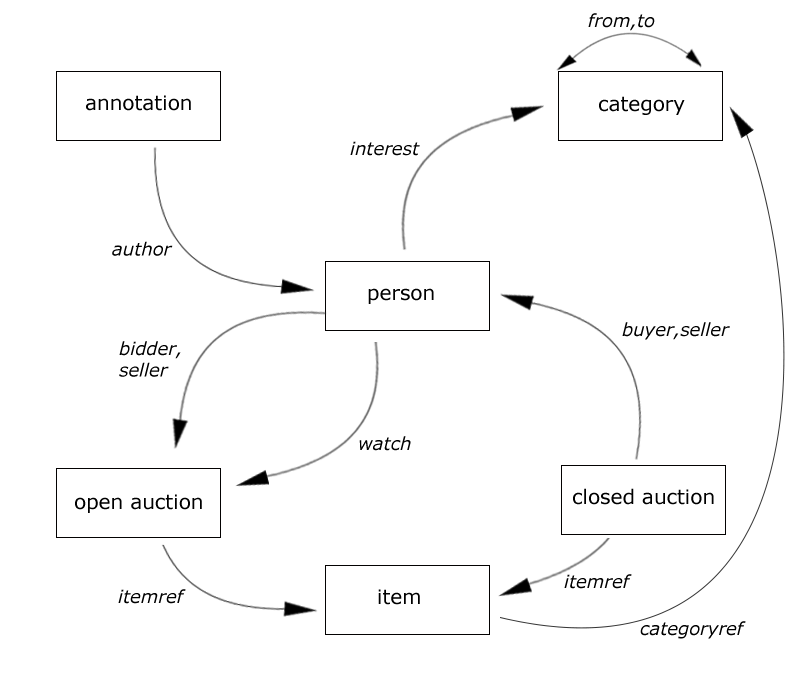
\includegraphics[width=0.40\textwidth]{img/xmark/101}{ %xmark-references.png
			\label{fig:xmark-reference}
		}
	}
	\centering
	\subfloat[Reference in \textit{XMark} dataset tree]{
		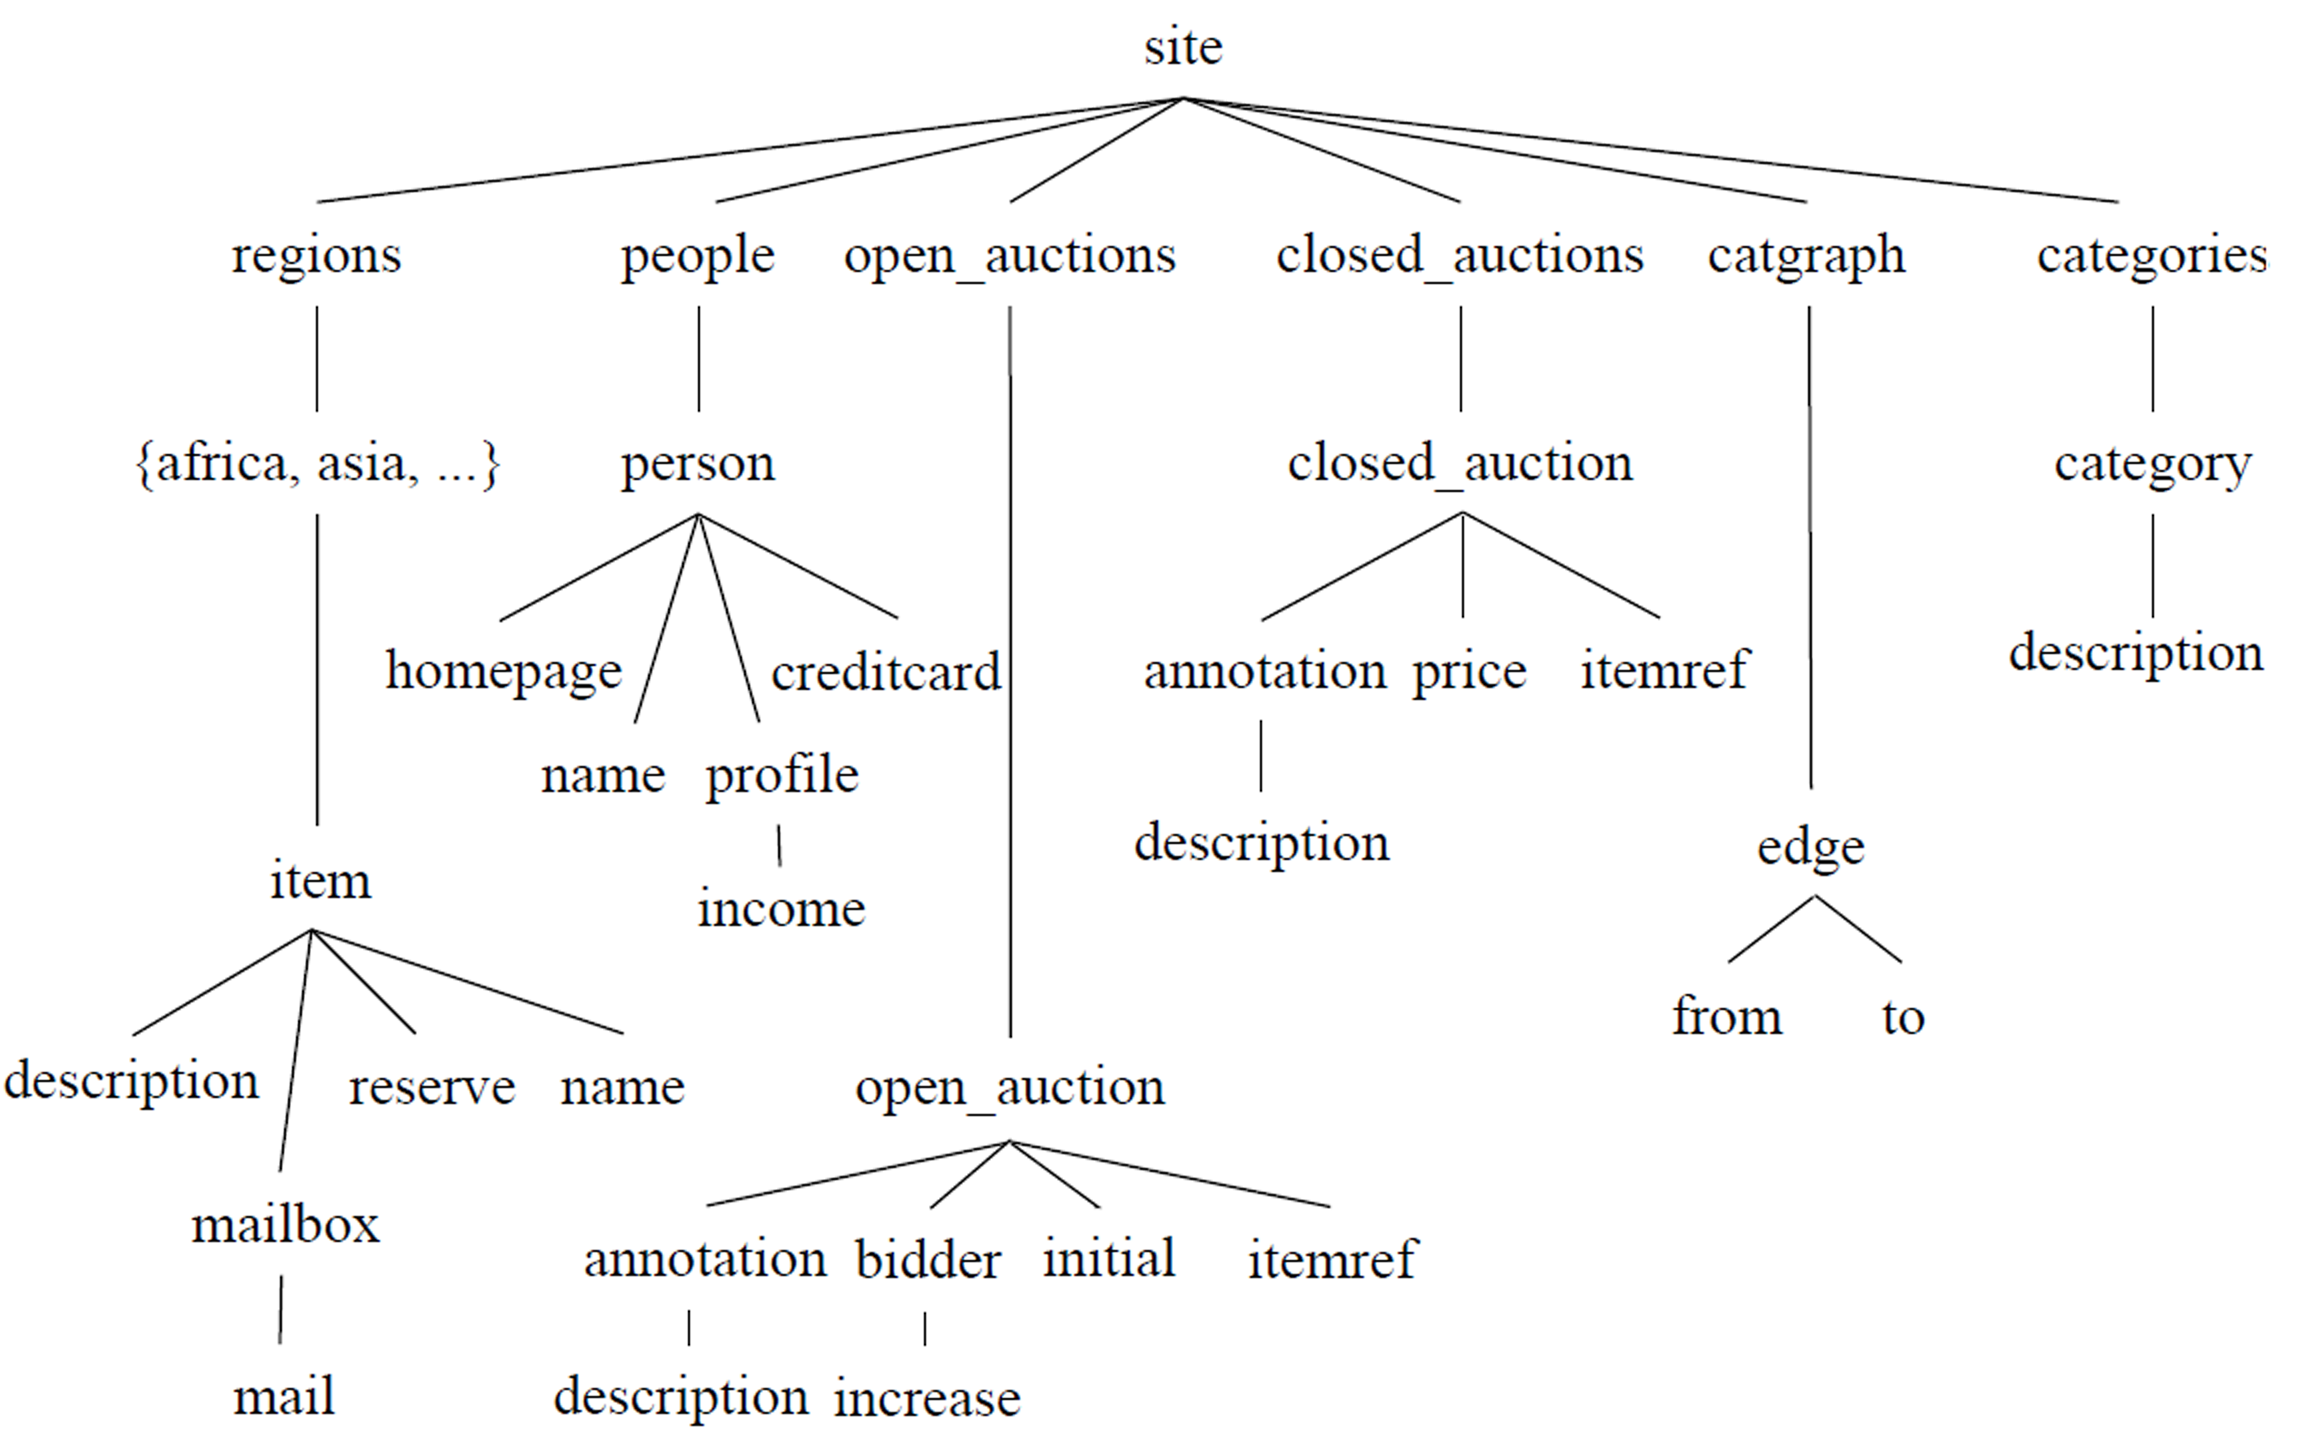
\includegraphics[width=0.4\textwidth]{img/xmark-tree.png}{
			\label{fig:xmark-tree}
		}
	}
	\caption{XMark data tree and reference~\citep{xmark/original}}
	\label{fig:xmark-tree-reference}
\end{figure}
\begin{figure}[H]
	\centering
	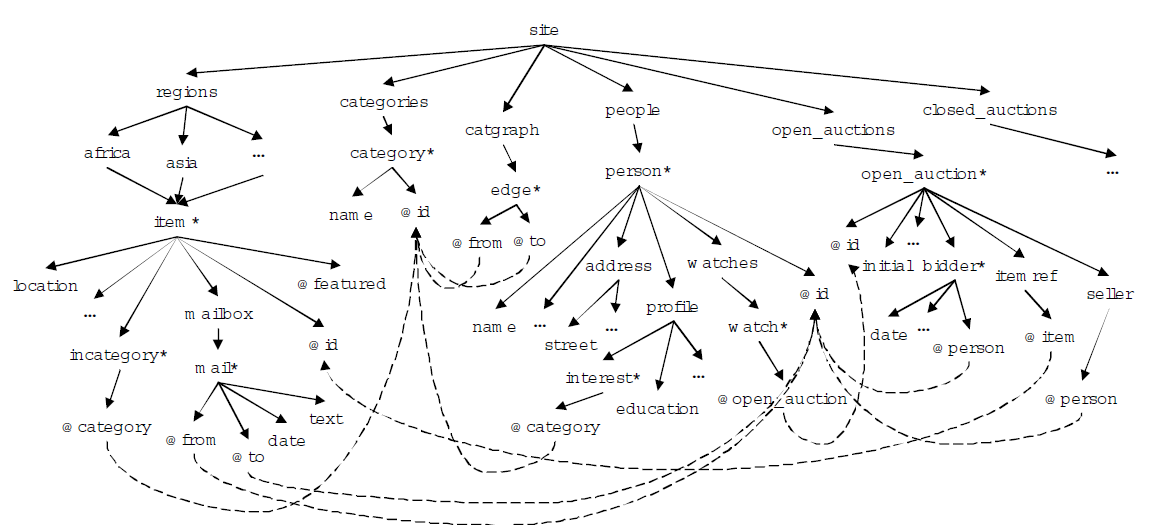
\includegraphics[width=0.90\textwidth]{img/xmark-schema-4}
	\caption{XMark ER-Diagram. Nodes, solid arrows, and dashed arrows represent schema elements (or attributes, with prefix '@'), structural links, and value links, respectively. Elements with suffix '*' are of SetOf type\citep{xmark/schema-sumerize}}
	\label{fig:xmark-schema}
\end{figure}

\subsection{XMark Queries}\label{xmark-queries}
The XMark project contains XQuery queries that focuses on the various aspect of language such as aggregation, reference, ordering, wildcard expressions, joins, user defined functions, etc.\citep{xmark/mlynkova2008xml}.The textual representation of 20 different XQuery expressions is reprinted in  Table~\ref{tab:xmark-queries}. These queries are divided into different categories  based on the  multiple functionalities of XQuery: 
\begin{enumerate}[label=\arabic*.]
\item  First category tests execution of exact match of string in specified path and consists of only query Q1.
\item It  helps to analyze order access of an XML document. Query Q2, Q3 and Q4 are grouped here.
\item  Query Q5 is evaluates the casting of a value.
\item Queries Q6 and Q7  evaluate regular path expressions.

\item This category investigates the referencing of a document to another and consists of query Q8 and Q9

\item Query Q10 reconstructs a complex results from the result of a query

\item Two queries, Q11 and Q12 are join query based on values.  The difference between this category's queries and reference queries Q8 and Q9 is that references are specified in DTD and may optimize with object identifiers whereas Q11 and Q12 are have join on the basis of values.

\item Query Q13  benchmarks the portion reconstruction of original XML document.

\item In this category the full text search  using single word is implemented. Q14 is in this category

\item The purpose of queries 15 and 16 is to observe the path traversals without using wildcards.

\item Query Q17 tests the ability to deal with missing values

\item This category deals with user defined functions and contains query Q18

\item The query Q19 is use to evaluate Sorting.

\item The last category observe the aggregation with the help of query 20.

\end{enumerate}

\begin {table}[htpb] 
\centering
\caption {The XMark queries. Source:\citep{xmark/original}}
\label {tab:xmark-queries}
\begin{tabular}{r|l}
	\hline
	Q1&Return the name of the person with ID 'person0'.\\
	\hline
	Q2&Return the initial increase of all open auctions.\\
	\hline
	Q3&Return the first and current increase of all open auctions whose current\\
	&increase is at least twice as high as the initial increase.\\
	\hline
	Q4&List the reserves of those open auctions where a certain person issued\\
	&a bid before another person.\\
	\hline
	Q5&How many sold items cost more than 40.\\
	\hline
	Q6&How many items are listed on all continents?\\
	\hline
	Q7&How many pieces of prose are in our database?\\
	\hline
	Q8&List the names of persons and the number of items they bought.\\
	&(Joins person, closed\_auction)\\
	\hline
	Q9&List the names of persons and the names of items they bought in Europe.\\
	&(Joins person\_auction, item)\\
	\hline
	Q10&List all persons according to their interest; use French markup\\
	&in the result.\\
	\hline
	Q11&For each person, list the number of items currently on sale whose\\
	&price does not exceed 0.02\% of the person's income.\\
	\hline
	Q12&For each richer-than-average person, list the number of items currently\\
	&on sale whose price does not exceed 0.02\% of the person's income.\\
	\hline
	Q13&List the names of items registered in Australia along with\\
	&their description.\\
	\hline
	Q14&Return the names of all items whose description contains the word 'gold'.\\
	\hline
	Q15&Print the keywords in emphasis in annotations of closed auctions.\\
	\hline
	Q16&Return the IDs of those auctions that have one or more keywords\\
	&in emphasis.\\
	\hline
	Q17&Which persons don't have a homepage?\\
	\hline
	Q18&Convert the currency of the reserve of all open auctions to\\
	&another currency.\\
	\hline
	Q19&Give an alphabetically ordered list of all items along with their location.\\
	\hline
	Q20&Group customers by their income and output the cardinality of each\\
	&group.\\
	\hline
\end{tabular}
\end {table}

		\subsection{XMark data into NoSQL database}\label{xmark-nosql}
			A synthetic XMARK dataset consists of a huge record in tree structure~\citep{xmark/VIST}. As mentioned in Section~\ref{xmark-dataset}, each subtree, \textit{regions}, \textit{people}, \textit{open\_auctions}, \textit{closed\_auctions}, \textit{catgraph} and \textit{categories} contain large numbers of instances that are indexed during database creation. At first, in most NoSQL database, the dataset cannot be a huge block but in fragmented form with each instances having it's own index structure. Besides this, NoSQL databases limits the size of a single document. For example, MongoDB has a limitation of 16 MB per document, the maximum size of documents allowed in RethinkDB is 64 MB and Couchbase Server can have value of a key upto 20 MB. The data model of NoSQL does not match single instance model of XML database.
\par 
To model XMark dataset into NoSQL, we have broken down the tree structure of XMark into set of sub-structure without losing the overall data. Each NoSQL database has their own data model, hence it is required to define a model for each of those databases separately.

The generalized concept of  XMark data into NoSQL databases is explained here but it might slightly differ from one another. 

All sub-trees \textit{regions}, \textit{people}, \textit{open\_auctions}, \textit{closed\_auctions}, \textit{catgraph} and \textit{categories} are the basic unit for the document fragmentation. Each of these sub-trees stores entities \textit{item}, \textit{person}, \textit{open\_auction}, \textit{closed\_auction} and \textit{category} respectively as mentioned in Section~\ref{xmark-dataset}. These entities represent the documents in NoSQL databases. In each document, one special field \textit{doctype} is added to represent the name of parent sub-tree. For example, in case of \textit{people} sub-tree, the value of \textit{doctype} is \textit{people}. This key/value set will be the part of a document as  given in Table~\ref{tbl:xmark-xml-json}(b). The \textit{doctype} has all-together six distinct values : \textit{categories}, \textit{catgraph}, \textit{people}, \textit{open\_auctions} and \textit{closed\_auctions}. There is an exceptional case for \textit{item} entities. It has \textit{regions} as grandparent and name of different regions like \textit{asia}, \textit{europe}, \textit{australia}, \textit{namerica}, \textit{samerica} etc. as the parent.  The \textit{doctype} for \textit{item} document will be \textit{regions} as other. To represent the name of regions like \textit{asia}, \textit{europe}, etc.,  one field with key \textit{regions} is added in each document. 
Table~\ref{tbl:xmark-item-type} illustrate the extra attribute added in each of document.

\begin{longtable}{c|c}
	\caption{ Extra attribute of a document in NoSQL}
	\label{tbl:xmark-item-type}\\
    {for \textit{person} and all other entities except \textit{item} } & {for \textit{item} which has region name \textit{asia}}\\
	\hline
\begin{minipage}{.4\textwidth}
\begin{lstlisting}[language=JSON]
{
	"doctype":"people"
}
\end{lstlisting}
\end{minipage} &
\begin{minipage}{.4\textwidth}
\begin{lstlisting}[language=JSON]
{
	"doctype":"regions",
	"regions":"asia"
}
\end{lstlisting}
\end{minipage}
\end{longtable}

A sample document of NoSQL database along with respective XMark document is illustrated in  Table~\ref{tbl:xmark-xml-json}. The conversion from XML to JSON is carried out using algorithms of Section~\ref{xml-to-json-migration} with one extra attribute "doctype" to represent the parent of a document. If an element in XML has siblings with same name, they are represented as an array in NoSQL document which is already mentioned in algorithm~\ref{algorithm-JSONXML}. As it can be seen, the \textit{person} of XMark is a document in NoSQL, it is not necessary to represent this attribute.  

\begin{longtable}{c|c}
	\caption{Example: XMARK data with id \textit{person0} in XML and JSON format }
	\label{tbl:xmark-xml-json}\\
	{\textit{person0}} in XML(a) & {\textit{person0}} in JSON for a NoSQL database(b)\\
	\hline
	\begin{minipage}{.4\textwidth}
\centering		
\begin{lstlisting}[language=XML,basicstyle = \tiny,label=code:xml-nosql-person0]
<people>
    <person id="person0">
       <name>Kasidit Treweek</name>
       <emailaddress>mailto:Treweek@cohera.com</emailaddress>
       <phone>+0 (645) 43954155</phone>
       <homepage>http://www.cohera.com/~Treweek</homepage>
       <creditcard>9941 9701 2489 4716</creditcard>
       <profile income="20186.59">
          <interest category="category251" />
          <interest category="category341"/>
          <education>Graduate School</education>
          <business>No</business>
       </profile>
    </person>
</people>
\end{lstlisting}	
	\end{minipage} &
	\begin{minipage}{.55\textwidth}
		\centering
		\begin{lstlisting}[language=JSON, basicstyle =\tiny, label=code:json-nosql-person0, numberstyle=\tiny]
{
	"id": "person0",
	<@\textit{"doctype": "people",}@>
	"name": "Kasidit Treweek",
	"emailaddress": "mailto:Treweek@cohera.com",
	"phone": "+0 (645) 43954155",
	"homepage": "http://www.cohera.com/~Treweek",
	"creditcard": "9941 9701 2489 4716",
	"profile": {
		"income": 20186.59,
		<@\textcolor{red}{
		"interest": [{
			"category": "category251"
		},{
			"category": "category341"
		}]}@>,
		"education": "Graduate School",
		"business": "No"
	}
}
		\end{lstlisting}
	\end{minipage}\\
\end{longtable}



\begin{comment}
\iffalse\fi
\begin{minipage}{.5\textwidth}
	\begin{tikzpicture}[%
	grow via three points={one child at (0.5,-0.7) and
		two children at (0.5,-0.7) and (0.5,-1.4)},
	edge from parent path={(\tikzparentnode.south) |- (\tikzchildnode.west)}]
	\node {\{asfdasfd\}}
	child { node [defi] {\textit{Schema\_ID}}}
	child { node [json] {xs:attribute}
		child { node [defi] {\textit{Attribute\_ID}}}
		child { node [attribute] {@name}}
		child { node [attribute] {@type}}
		child { node [attribute] {@fixed}}
		child { node [attribute] {@default}}
	};
	\end{tikzpicture}
\end{minipage}

\end{comment}


			\subsubsection{XMARK dataset in MongoDB}\label{xmark-mongodb}
				In MongoDB, collections consist of group of documents with similar structure. Therefore, the data modeling concept of Section~\ref{xmark-nosql} has to be modified marginally. The documents are grouped with their \textit{doctype} from Section~\ref{xmark-nosql}. Each \textit{doctype} represent a collection, there are all together 6 collections. The field \textit{doctype} is already represented as collections, it is removed from all documents.  
For \textit{item} entity,  field \textit{regions} does not change. The \textit{\_id} is the primary index of a document in MongoDB, the identifier attribute of the XMark data \textit{id} is renamed to \textit{\_id} for default indexing.  \textit{closed\_auctions} and \textit{catgraph} do not have an identifier attribute \textit{id}, therefore, system will automatically generate the \textit{\_id} in these collections.
A typical example of MongoDB document for person with identifier \textit{person0} is given in Figure~\ref{code:mongodb-person0}.	

\begin{figure}[hbt]
\begin{lstlisting}[language=JSON, basicstyle =\scriptsize]
    {
    	<@\textbf{"\_id": "person0",}@>
    	"name": "Kasidit Treweek",
    	"emailaddress": "mailto:Treweek@cohera.com",
    	"phone": "+0 (645) 43954155",
    	"homepage": "http://www.cohera.com/~Treweek",
    	"creditcard": "9941 9701 2489 4716",
    	"profile": {
    		"income": 20186.59,
    		"interest": [
    			{"category": "category251"},
    			{"category": "category341"}
    			],
    		"education": "Graduate School",
    		"business": "No"
    	}
    }
\end{lstlisting}
\caption{MongoDB document of XMark data in \textit{people} collection}
\label{code:mongodb-person0}
\end{figure}
			\subsubsection{XMARK dataset in Couchbase}\label{xmark-couchbase}
				\begin{figure}[h]
\begin{lstlisting}[language=JSON,  basicstyle =\scriptsize]
{
	"id":  "item1000",
	"doctype":  "regions",
	"regions":  "africa",
	"name":  "duteous nine eighteen" ,
	"payment":  "Creditcard" ,
	"quantity": 1 ,
	"shipping":  "Will ship internationally, See description for charges" ,
	"incategory": [
		{
		"category":  "category0"
		}
	] ,
	"mailbox":[],
	"description":{ }
}
\end{lstlisting} 
\caption{Couchbase pseudo-document of the XMark data for item with id \textit{item1000}}
\label{code:couchbase-item0}
\end{figure}

Couchbase does not have the concept of grouping documents like \textit{collections} in MongoDB  or \textit{tables} in RethinkDB. 
Therefore, the data model of Section ~\ref{xmark-nosql} is applied without modification.
 All the documents are stored in a single bucket with identifier attribute \textit{id} as a document key. An \textit{id} will be manually generated for the documents without identifier.
 An example of Couchbase document is illustrated in Figure~\ref{code:couchbase-item0}

			\subsubsection{XMARK dataset in Rethinkdb}\label{xmark-rethinkdb}
				RethinkDB stores the documents inside a table which is identical to the collection in MongoDB. 
The documents are grouped according to their \textit{doctype} and store in a table.
Each \textit{doctype} of \ref{xmark-nosql} is represented as an individual table. 
The tables \textit{regions}, \textit{people}, \textit{open\_auctions}, \textit{closed\_auctions}, \textit{catgraph} and \textit{categories} contains the respective documents as of \textit{doctype}. Hence the attribute \textit{doctype} is removed from all documents.  \textit{id} is the primary key and any document without \textit{id} field is automatically added as an identifier during the time of insertion. Figure~\ref{code:rethindb-person0} shows a document with id \textit{person0} in \textit{people} table.


\newbox\rethinkdbXmarkDocument
\begin{lrbox}{\rethinkdbXmarkDocument}
\begin{lstlisting}[language=JSON,basicstyle =\scriptsize]

	{
		 <@\textbf{"id": "person0"}@>,
		"name": "Kasidit Treweek",
		"emailaddress": "mailto:Treweek@cohera.com",
		"phone": "+0 (645) 43954155",
		"homepage": "http://www.cohera.com/~Treweek",
		"creditcard": "9941 9701 2489 4716",
		"profile": {
			"income": 20186.59,
			"interest": [
			    { "category": "category251" },
				{"category": "category341"}
			],
			"education": "Graduate School",
			"business": "No"
		}
	}
\end{lstlisting}
\end{lrbox}


\newbox\rethinkdbXmarkChart
\begin{lrbox}{\rethinkdbXmarkChart}
\begin{tikzpicture}[grow'=right,level distance=1.25in,sibling distance=.25in, font=\scriptsize]
\tikzset{edge from parent/.style= 
            {thick, draw, edge from parent fork right},
         every tree node/.style=
            {draw,minimum width=1in,text width=1in,align=center}}
\Tree 
    [. Database 
        [.{regions}
            [.{... } ]
        ]
        [.people
            [.{person0 } ]
        ] 
        [.{open\_auctions}
            [.{... } ]
        ]
        [.{closed\_auctions}
            [.{... } ]
        ]
        [.{catgraph}
            [.{... } ]
        ]
        [.{categories}
            [.{... } ]
        ]
    ]
    
\end{tikzpicture}
\end{lrbox}

\begin{figure}[hhtp]
\centering
\subfloat[Database, tables and documents in RethinkDB] {
    \usebox\rethinkdbXmarkChart
    \label{xmark-rethinkdb-tree}
}
\\
\centering
\subfloat[RethinkDB document \textit{person0} in \textit{people} table ] {
        \usebox\rethinkdbXmarkDocument
        \label{code:rethindb-person0}
}

\caption{XMark data in RethinkDB}
\label{xmark-rethinkdb-figure}
\end{figure}
	%this section have to move to in conclusion and future work
	%\section{Related work}
	\chapter{Benchmarking}\label{ch:benchmarking} %Performance/Experiments
	\section{Benchmarking configurations}
	For benchmarking, we have used same hardware configuration for all four databases in single mode. All the test in this chapter is done using  Linux 3.13.0-49 (Ubuntu 14.04, 64bit) with Intel Core i3 with 4GB RAM and 256GB SSD machine.
Table~\ref{benchmark-configuration-table} describes hardware and software information used for benchmarking. 
\begin{table}[h]	
	\centering
	\caption{Reportable Benchmark Information}
	\begin{tabular}{|c|c|c|c} 
		\hline
		Hardware: & \multicolumn{3}{|c|}{CPU: Intel core i3, RAM: 4GB, SSD:256GB  } \\
		\hline
		Software: & \multicolumn{3}{|c|}{OS: Linux 3.13.0-49(Ubuntu 14.04), 64 bit} \\
		\hline
		DBMS and Version: & \multicolumn{3}{|c|}{ BaseX: 8.1, Mongodb:2.6.9, Rethinkdb:2.0,Couchbase Server:3.0 } \\
		\hline
		Other Software: & \multicolumn{3}{|c|}{Nodejs: v0.12.2, Java:1.7.0\_80 } \\
		\hline
	\end{tabular}	
	\label{benchmark-configuration-table}
\end{table}
There are certain queries that are dependent on drivers. Those queries are tested through the client-server architecture for all databases. MongoDB, Couchbase and RethinDB natively support Node.js and JavaScript, therefore, these queries are examined through Nodejs version  v0.12.2. For BaseX, the client-server architecture is used with Java 1.7.0. Basex 8.1, MongoDB 2.6.9, Couchbase 3.0 and RethinkDB 2.0 are the versions of databases used for the comparison. 
    \section{Database Queries}
        All the XQuery expressions are translated into NoSQL database queries based on the output result. In case of availability of secondary indexes, they have been created and utilized for efficient result. There are some problems for following queries:
\todo{why not Q4?}
\begin{itemize}
\item Q4 and Q7 cannot be applied to NoSQL databases. These queries will be skipped during the measurement and analysis. In Q7, XPath  wild cards cannot be used in NoSQL databases, which makes it impossible to perform the query. 

\item In Q14, full text search is measured in XQuery. MongoDB, Couchbase and RethinkDB do not support full text search, therefore  sub-string search is performed in these databases. 
\end{itemize}

\subsection{XMark Queries in MongoDB}

In MongoDB, all the possible query methods have been implemented to get the same result as of XQuery.  For an example, the \textit{find()} function can be used for Q1 to get result. As we can see in  Code~\ref{mongo-xmark-q1}, the collection is filtered with default index \textit{\_id}  and the second parameter specifies the \textit{name} field to be retrieved.  For advanced queries, the aggregation pipeline and mapreduce are used. 

As mentioned in ~\ref{nosql-mongodb}, MongoDB has no support for  join queries. All the queries that need more than one collection  Q8, Q9, Q10, Q11 and Q12  are processed through \textit{mongo shell}. Secondary indexes are created only when queries can be optimized. Without indexes, MongoDB has to scan every document in a collection to match the criteria of the query. MongoDB secondary index can be created by using \textit{createIndex} function as in Code~\ref{mongodb-create-index}. Some of the important queries are explained here:

\begin{itemize}
\item Q1 implements the default index \textit{\_id}. Firstly, the collection is filtered then \textit{name} field is specified for selection. 

\item for Q2 and Q3, firstly, two indexes in fields \textit{initial} and \textit{"bidder.increase"} of collection \textit{open\_auctions} are created. With various steps of aggregation pipeline the result is returned.

\item A comparison operator is implemented in Q5 that can be easily optimized with index. A secondary index is created in field \textit{price} of \textit{closed\_auctions} collection. 
\item According to our data model for MongoDB, Q6 counts the number of documents in the collection \textit{regions}.
\item In Q8, joins between two collections \textit{people} and \textit{closed\_auction} has been performed. The field \textit{buyer.person} has been indexed, therefore the \textit{person} search is efficient. 
The Q9 implements index of Q8 and a new index on \textit{regions} field of \textit{regions} collection is added which is also utilized in Q13.
\item For Q10, another index on \textit{profile.interest} field of \textit{people} collection is created. A helper function is used to join and format the data.
\item For Q14, a \textit{text index} is created in a collection \textit{regions} that allow to search by any sub-strings in whole collection. 
\item The result of Q15 and Q16 do not match the exact result of XQuery, because  XQuery uses  XPath whereas MongoDB do not.

\item The quey Q18 implements user-defined function. In MongoDB, it has to process two steps: A used defined function is created and stored in database system document. Then, through mapreduce it is called. Table~\ref{tbl:mongodb-q18} illustrates Q18 using mapreduce.

\item For Q19, a secondary index on field \textit{location} of collection \textit{regions} is created.
It is used for sorting the data by the \textit{location}. 
\item
The final query Q20 based on aggregations. This query in mapreduce  is much simpler than aggregation pipeline.
\end{itemize}
Full list of MongoDB queries and index can be found in ~\ref{mongodb-query-list}

\begin{figure}
\centering
\begin{lstlisting}[language=JSON, caption=XMark Query Q1 in MongoDB, label=mongo-xmark-q1]
		db.people.find({_id:"person0"},{_id:0,"name":1});
\end{lstlisting}

\centering
\begin{lstlisting}[language=JSON, caption=MongoDB secondary Index, label=mongodb-create-index]
             db.closed_auctions.createIndex({regions:1})
\end{lstlisting}
\end{figure}



\begin{longtable}{c|c}
    \hline
	\caption{ User-defiend function and implementation in MongoDB(Q18)}
	\label{tbl:mongodb-q18}\\
    {function } & {map-reduce}\\
	\hline
\begin{minipage}{.4\textwidth}
\begin{lstlisting}[language=JSON,basicstyle =\scriptsize]
    db.system.js.save({ 
        "_id": "reserve", 
        "value": 
            function(a){ 
                return 2.20371*a; 
            } 
    })
\end{lstlisting}
\end{minipage} &
\begin{minipage}{.4\textwidth}
\begin{lstlisting}[language=JSON,basicstyle =\scriptsize]
db.open_auctions.mapReduce(
    function() {
       if(this.reserve){
        emit(this._id, reserve(this.reserve));
       }    
    },
    function(key,values) {
        return Array.sum(values);
    },
    { "out": { "inline": 1 } }
 );
\end{lstlisting}
\end{minipage}
\end{longtable}


\subsection{XMark Queries in Couchbase}
 In Couchbase, everything is queried with the views. The output of the views are queried through programming interface. For each query, the \textit{doctype} should be checked.  All XMark queries have been queried and evaluated through Node.js in Couchbase. Some of the important queries are illustrated here:
 
 \begin{itemize}
 \item Q1 is a simple query where the map function emits \textit{id} and \textit{name} of document if the condition is matched.
 \item In Q2 and Q3 are deeper array and object processing for couchbase.
 \item Both Q5 and Q6 use the built-in reduce function of views \textit{\_count}.
 \item The join operation in Couchbase is bit complicated as compare to other NoSQL database. Each \textit{doctype} should have a view and it can be implemented multiple times. For example, in case of Q11 and Q12, view on \textit{open\_auctions} can be used for both both queries.  The join operation is completed using programming interface. The Q8 contains two views, one selects the \textit{id} and \textit{name} field from \textit{people}. other view aggregates doctype  \textit{closed\_auctions} using reduce function with query option \textit{group\_level=1}. Finally, both views are combined using Node.js. 
 \item In Q14, the \textit{description} field in \textit{regions} are converted into string  that makes substring search is possible.
 
 \item In Q18, for a user-defined function implementation, a JavaScript function is created at map section and called at during emit. 
 \item In Q19, a query parameter \textit{descending} have to make false for result in ascending order. 
 \end{itemize}
 
 Table~\ref{tbl:couchbase-q20} illustrates a sample example of XMark  Q20 with  mapreduce functions and the query parameters. The full list of Couchbase Mapreduce can be found in ~\ref{couchbase-query-list}.

\begin{longtable}{c|c|c}
	\caption{ XMark query Q20 in Couchbase Server}
	\label{tbl:couchbase-q20}\\
    {map} & {reduce} & {query}\\
	\hline
\begin{minipage}{.5\textwidth}
\begin{lstlisting}[language=JSON,basicstyle =\scriptsize]
function (doc, meta) {
    if(doc.doctype=="people"){
      var income = (doc.profile && doc.profile.income) ? 
                doc.profile.income : 0;
      if(income >= 100000 ){
    	 emit("preferred",1);
      }else if(income < 100000 && 
               income >= 30000) {
        emit("standard",1);
      }else if(income < 30000 &&
           income > 0 ){
       
        emit("challenge",1);
      } else {
       emit("na",1);
      }
    }
  }
\end{lstlisting}
\end{minipage} &
\begin{minipage}{.15\textwidth}
\begin{lstlisting}[language=JSON,basicstyle =\scriptsize]
     _sum
\end{lstlisting}
\end{minipage} &
\begin{minipage}{.2\textwidth}
\begin{lstlisting}[language=JSON,basicstyle =\scriptsize]
     group_level=1
\end{lstlisting}
\end{minipage}
\end{longtable}

\subsection{XMark Queries in RethinkDB}

In RethinkDB, the performance of a read query can be improved through the secondary indexes. In XMark queries,  wherever possible, these indexes are utilized to improve the performance. The index has to be defined in the query and can be used only in one of the four functions \textit{getAll()}, \textit{between()}, \textit{eqJoin()} and \textit{orderBy()}. Table~\ref{tbl:rethinkdb-index-query} illustrates an example of creating a secondary index and its usage in a query.
\begin{longtable}{c|c}
	\caption{ RethinkDB secondary index and Query for Q13}
	\label{tbl:rethinkdb-index-query}\\
    {Index} & {Query}\\
	\hline
\begin{minipage}{.3\textwidth}
\begin{lstlisting}[language=JSON,basicstyle=\scriptsize]
    r.table("regions")
        .indexCreate("regions")
\end{lstlisting}
\end{minipage} &
\begin{minipage}{.5\textwidth}
\begin{lstlisting}[language=JSON,basicstyle=\scriptsize]
r.table("regions")
.getAll("australia",{index:"regions"})
    .map({  
       item:{  
          name:r.row("name"),
          description:r.row("description")
       }
    })
\end{lstlisting}
\end{minipage}
\end{longtable}
Some of the importain queries in RethinkDB explained here.


For query Q1, the document can be retrieved by the primary key \textit{id} using \textit{get()} function.  ReQl has more features for arrays and objects compare to  other NoSQL databases that helped in Q2 and Q3. Due to native support for joins between table, join queries are more flexible in RethinkDB. An index \textit{buyer\_person} is created in field "buyer.person" of \textit{closed\_auctions} table for Q8. Similarly, the Q9 can be improved by creating indexes in the tables \textit{regions} and \textit{closed\_auctions}. Other queries like Q13 and Q19 is also evaluated using indexes. For substring search in Q14, the value of  field \textit{description} is converted into text and then it is matched for the sub-string. All the queries and indexes are used for RethinkDB is given in ~\ref{rethinkdb-query-list}.

    \section{Results and Analysis}
        In this section, we will focus on the analysis of different databases based on the  evaluation of XMark queries. BaseX, Mongodb, Couchbase and RethinkDB are  completely different database system  with their own data model and different query languages. Even all the NoSQL databases have different structures and query model.  Due to their complete different nature, a query of a database would perform better than others if data was normalized according their specified data model then our requirements. For example, BaseX would probably perform better if the data was normalized as well. Therefore, our goal is not to compare queries between theses databases but evaluates the results individually.  Each databases has been tested in 6 different size XMark data as mentioned in ~\ref{xmark}. Firstly, we will analyze result of each of the four systems. Finally, we will check the all database together in a single figure for 111MB dataset. 

\subsection{MongoDB}
Figure~\ref{fig:xmark-result-mongodb-all} presents the time measurement of XMark queries in MongoDB. MongoDB automatically uses all the free memory of a machine for its cache. But this usage is dynamic and if other processes need the Server's RAM, it handover such cached memory to other process. Hence, the result of XMark queries might depends on the other processes running in the machine.  The result of the queries will be explained below:
\begin{itemize}
\item The simplest query Q1 was the most efficient query for all instances of database and executed less than 4ms. Conditional operator on the default index \textit{\_id} made it faster.
\item Q3 and Q4 were relatevely slower queries due to multi-stage array processing with aggregation pipeline. Even two secondary indexes were used, the performance of these queries could not be competitive to other systems. 
\item The \textit{count} operation in MongoDB with simple filtration is comparatively faster than other NoSQL databases, Q5 and Q6 are used to count the number of documents in a collection with criteria. In Q5, the secondary index in field \textit{price}  helped to accelerate the performance. Figure~\ref{fig:xmark-mongodb-index-noindex} clarifies the efficiency of two queries Q5 and Q13 where the execution time improved exponentially after the indexes. In Q6, just the \textit{count()} operation in a collection due to data model defined in ~\ref{xmark-mongodb} made better performance possible. 

\item Among the join queries, Q8 and Q9 generated the best result in case of execution time among the other system, once again the indexes created in these two queries improved the performance. But in case of Q10, complex result generations with joins could not be completed for two databases, a large output with many new fields made the query inefficient. The value join queries in Q11 and Q12 has to deal with many read operations due to manual join, therefore these queries also did not perform well.

\item The secondary index in Q13 helped to keep execution time low, As mentioned earlier the Fig.~\ref{fig:xmark-result-mongodb-13} shows the time consumed by Q13  with and without index. Q14 is used to search for sub-string instead of full text search of XQuery, the relative performance was decreased when the size of database in increased.

\item The structures of the queries in Q15 and Q16 are complex in all NoSQL databases including MongoDB because of deep path in XQuery and has to process many array and object elements. The results produced in these queries were not exactly same as of XQuery but the performance was in the same level and the size of database did not have greater effect. The result of Q17 was similar to that of other systems but performance of Q18 has been decreased when database get bigger. 
Q19 returned result in new field \textit{item} that reduces the performance because  MongoDB has to use aggregation pipeline for new field.  The Query would be much more faster if the result would be return without new element using \textit{find} function. 
\item Finally, the query Q20 groups, categories them and returns cardinalities. As the database get bigger query became slower. 
\end{itemize}
\begin{figure}
	\centering
	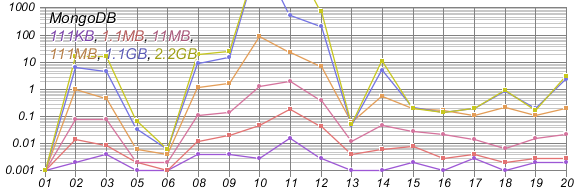
\includegraphics[width=0.95\textwidth]{img/result/mongodb/mongodb-all}
	\caption{XMark queries in MongoDB}
	\label{fig:xmark-result-mongodb-all}
	
\end{figure}	
\begin{figure}
	\centering
	\subfloat[Q5]{
		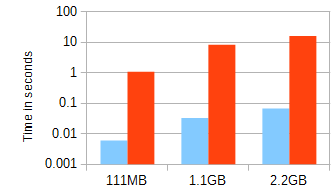
\includegraphics[width=0.4\textwidth]{img/result/mongodb/mongodb-q5-index-noindex}
		\label{fig:xmark-result-mongodb-5}
	}
	\centering
	\subfloat[Q13]{
		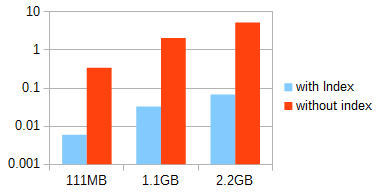
\includegraphics[width=0.4\textwidth]{img/result/mongodb/mongodb-q13-index-noindex}
		\label{fig:xmark-result-mongodb-13}
	}
	\caption{MongoDB queries with and without secondary index in different database instances}
	\label{fig:xmark-mongodb-index-noindex}
\end{figure}

\subsection{Basex}
The results of all six different databases in BaseX is shown in figure~\ref{fig:xmark-result-basex-all}. All the queries were tested with text, attribute and full text indexes. The query Q1 utilize the attributes index and return result a single result. This query was completed in less than 5mm in all databases. The query Q2 and Q3  with positional predicates took longer time if the the size of database is increases. The queries Q5 and Q6 uses count operation and both were relatively faster. As we've seen previous section, these queries performed better in MongoDB than in BaseX. Among the join-queries,  Q11 and Q12 could not be completed in defined time frame for databases bigger than 11MB. For reference join on attributes values defined in Q8 and Q9, the attribute index is utilized to get result. The time taken by these two queries is  similar to that of MongoDB.  The full text search query Q14 was slightly affected by the size of database. The queries Q15-Q17 implements the location paths, with similar performances and query Q18  implements user defined function for calculation. Q19 consumes most of resources for sorting for data. This query is faster in Mongodb compare to BaseX. Finally, the aggregation query Q20 produces constant result in all databases instances. 
\begin{figure}
	\centering
	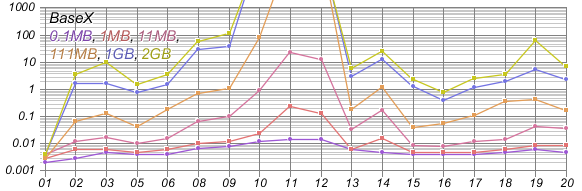
\includegraphics[width=0.95\textwidth]{img/result/basex/basex-all}
	\caption{XMark queries in BaseX}
	\label{fig:xmark-result-basex-all}
\end{figure}

\subsection{RethinkDB}
All the time evaluation of XMark queries in RethinkDB is given in Fig.~\ref{fig:xmark-result-rethinkdb-all}. 
\begin{itemize}
\item Query Q1 is consume more time compare to MongoDB and BaseX in average.
 \item  
  RethinkDB is able to handle arrays better ways than other NoSQL databases. Chains of queries can be used as a pipeline but unlike MongoDB's pipeline that produces result in multiple stages, RethinkDB runs a query on a server and once, hence it has been seen that queries Q2 and Q3 produces better result compare to MongoDB. 
 \item
 Queries Q5 and Q6 were comparatively slow in  RethinkDB. Firstly, MongoDB uses secondary index on Q5, but RethinkDB cannot be used a index in \textit{filter()} function. Secondly, the \textit{count()} operation in RethinkDB is always slow due to stream properties. It executes everything in server, most of the stream operations \todo{explain stream/lazy operation in introduction} including \textit{filter} runs lazily. The \textit{run} functions returns the results as soon as the first block of data is available, it does not load whole table data  at once. It will load rest of data as clients iterate over the cursor, therefore it does not keep much memory at once. In case of \textit{count()}, the query has to wait until all the data is loaded. 
 \item As we have mentioned the support of join query in ~\ref{xmark-rethinkdb}, RethinkDB was not able to take advantages of native joins except query Q11 and Q12. The join operation in Q8, Q9 and Q10 were similar in case of time measurement with rest of system. Q10 is slower due to large output and many new fields. 
 \item In query Q13, index is utilized on \textit{regions} field of the table that produces comparable result to MongoDB but better than BaseX. Queries Q14-Q19 are returned similar result except in Q15, due to many array sand object operations. 
\item The query Q20 was once again slow in RethinkDB due to cardinalities at the end of the query. All the grouping and categorizing operations were a lot faster than counting at the end. 
\end{itemize}

\begin{figure}
	\centering
	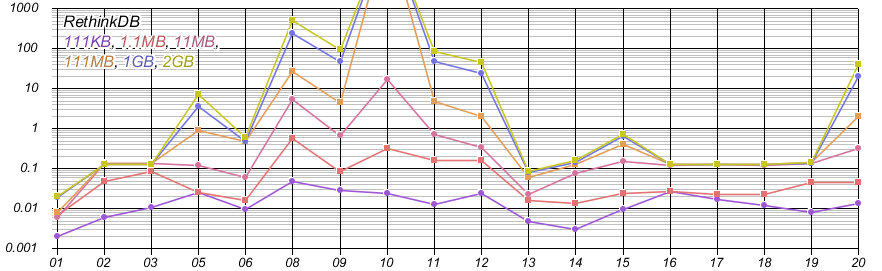
\includegraphics[width=0.95\textwidth]{img/result/rethinkdb/rethinkdb-all}
	\caption{XMark queries in RethinkDB}
	\label{fig:xmark-result-rethinkdb-all}
\end{figure}

\subsection{Couchbase}
Each Couchbase bucket is assigned RAM quota for caching data, therefore, the performance of a query depends on the amount of RAM allocated at the time of bucket creation. Figure~\ref{fig:xmark-result-cb-all} explains the query the performance of individual queries\todo{put all database images}. There were not any extraordinary phenomenon in Couchbase server.  Query Q1-Q3  were similar that of RethinkDB but Q5 and Q6 had produced comparatively better result due to its pre-defined reduce function \textit{\_count} in mapreduce. All the join queries were executed successfully in given time frame. Queries Q15-Q16 were performed slightly  better than that of other databases due to the JavaScript in map function. Another best result in Couchbase is aggregation query Q20, which is able to use pre-defined \textit{\_sum} in reduce part of Mapreduce. 

\begin{figure}
	\centering
	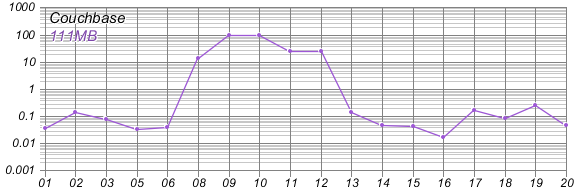
\includegraphics[width=0.95\textwidth]{img/result/cb/cb-all}
	\caption{XMark queries in Couchbase}
	\label{fig:xmark-result-cb-all}
\end{figure}

\subsection{Conclusion}
Even though our aim is not directly compare query performance in different systems, it would be interesting to see how these queries look like together. Figure~\ref{fig:xmark-result-1-all-new} illustrates all the queries for different database systems together for 111MB XMark data instance. MongoDB and BaseX have produced the best result in Q1. In Q2 and Q3, all database except MongoDB  had an identical result but in Q5 and Q6 MongoDB was the clear leader followed by Couchbae and BaseX, whereas RethinkDB was lagged behind other databases. In the join queries, the results produced by different databases were mixed in nature. MongoDB and BaseX were relatively better in Q8 and Q9 followed by Couchbase and RethinkDB. In Query Q10, the RethinkDB was failed to return result in given time frame but all other databases has identical results. The value join queries Q11 and Q12 were the best queries for RethinkDB followed by MongoDB and Couchbase but BaseX could not complete the result. Even the Q13 has similar results for all systems, RethinkDB had generated the best performance followed by MongoDB due to their efficient indexes. The FT search query Q14 is substring search for NoSQL databases, so that the query look little bit faster on them. The complex path queries Q15 and 16 Basex has better result with Couchbase than RethinkDB and MongoDB.
Q17-Q19 result are identical but in Q20 the Couchbase was the leader followed by Basex, MongoDB and RethinkDB. 
\\
\\
It has been seen that the NoSQL queries that were able to use secondary indexes performed better than BaseX with some exception. Even though some NoSQL do not support join queries, the result they produces are competitive in nature. The reason was favourable data model defined for those databases compare to BaseX and efficient read operation they produces. BaseX would probably perform better if the queries were optimized or data were normalized.  

\begin{table}[H]
\tiny
\begin{tabular}{|c|c|c|c|c|c|c|c|c|c|c| c|c|c|c|c|c|c|c|c|c|c|  } 
   db &  1 & 2 & 3 & 5 & 6  & 8 & 9 & 10  & 11 & 12 & 13 & 14 & 15 & 16 & 17 & 18 & 19 & 20 \\
 \hline
M\hbox{\pdfliteral{1 1 0 rg}\vrule height2mm width2mm depth0mm\pdfliteral{0 g}} & .00 & .75 & .78 & .01 & .00 & 1.17 & 1.65 & 87.25 & 23.13 & 7.21 & .05 & .55 & .20 & .17 & .11 & .22 & .11 & .21 \\
B\hbox{\pdfliteral{0 1 0 rg}\vrule height2mm width2mm depth0mm\pdfliteral{0 g}} & .04 & .19 & .17 & .10 & .19 & 2.31 & 2.43 & 89.36 & udf & udf & .36 & 1.23 & .08 & .08 & .15 & .36 & .52 & .19 \\
C\hbox{\pdfliteral{1 0 0 rg}\vrule height2mm width2mm depth0mm\pdfliteral{0 g}} & .04 & .14 & .08 & .03 & .04 & 13.2 & 98.1 & 94.1 & 24.1 & 26.1 & .13 & .05 & .04 & .02 & .17 & .09 & .27 & .05 \\
R\hbox{\pdfliteral{0 0 1 rg}\vrule height2mm width2mm depth0mm\pdfliteral{0 g}} & .01 & .14 & .14 & .94 & .68 & 26.76 & 4.53 & .00 & 4.80 & 2.10 & .02 & .18 & udf & .13 & .13 & .13 & .14 & 2.04 \\
\end{tabular}
\end{table}
\begin{figure}[H]
	\centering
	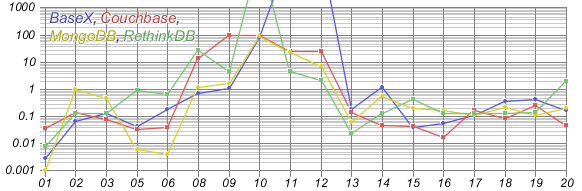
\includegraphics[width=0.85\textwidth]{img/result/1/1-all-new}
	\caption{XMark queries of 111MB data in all databases }
	\label{fig:xmark-result-1-all-new}
\end{figure}

























********** end here ******************


Figure~\ref{fig:xmark-result-basex-all} presents the time measuremnt of  XMark queries in BaseX. As mentioned earlier section, Q4 and Q7 are skipped because these queries cannot be translated into other NoSQL databases.  
	
We are using different charts for each of these databases instead of combine all the databases in a single chart. The queries are represented in x-axis with execution time in seconds is shown y-axis with limit 100 seconds. Queries Q4 and Q7 excluded in chart because they cannot be applied in NoSQL databases.


\begin{figure}[H]
	\centering
	\subfloat[BaseX]{
		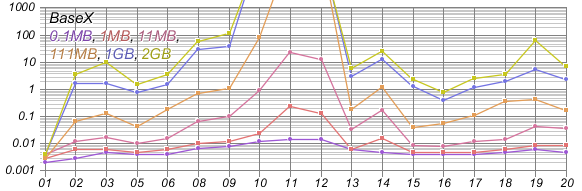
\includegraphics[width=0.95\textwidth]{img/result/basex/basex-all}
		\label{fig:xmark-result-1-basex}
	}\\
	
	\centering
	\subfloat[MongoDB]{
		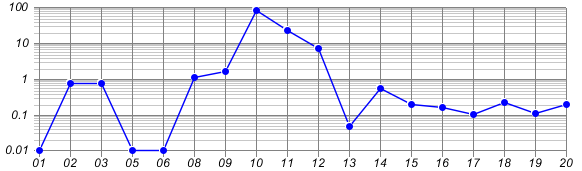
\includegraphics[width=.95\textwidth]{img/result/1/mongo}
		\label{fig:xmark-result-1-mongo}
	}\\
	
	\centering
	\subfloat[RethinkDB]{
		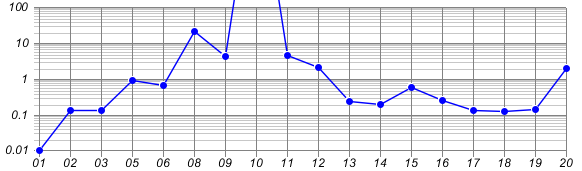
\includegraphics[width=.95\textwidth]{img/result/1/rethink}
		\label{fig:xmark-result-1-rethink}
	}\\
	
	\centering
	\subfloat[Couchbase]{
		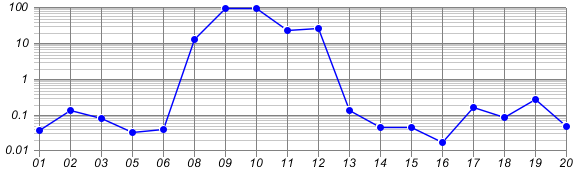
\includegraphics[width=.95\textwidth]{img/result/1/cb}
		\label{fig:xmark-result-1-cb}
	}
	
	
	\caption{Processing of XMark Queries on 111MB XMark instance}
	\label{fig:xmark-result-1-all}
\end{figure}
\begin{comment}
\begin{figure}[H]
	\centering
	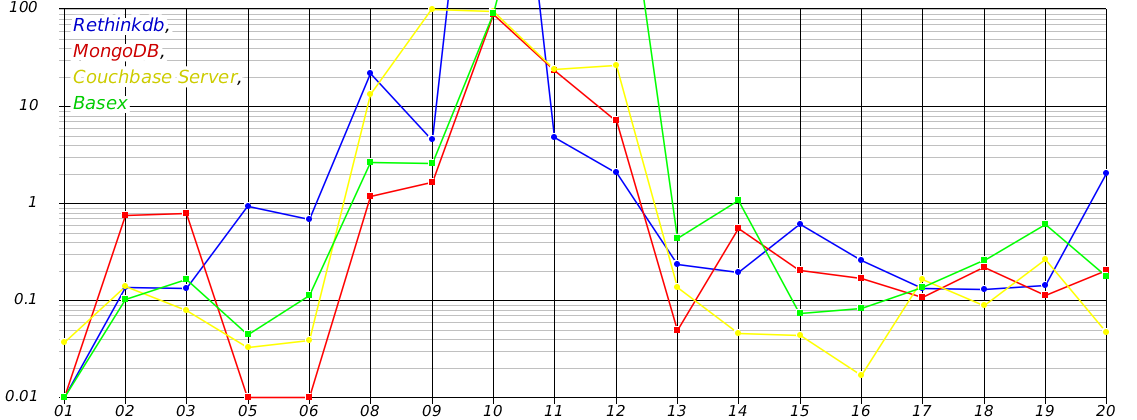
\includegraphics[width=1\textwidth]{img/result/1/all-2-2}
	\caption{Processing of Queries on 111MB XMark instance  in differet databases}
	\label{fig:xmark-result-all}
\end{figure}
\end{comment}


The result of individual queries will be explained here: 
 \begin{itemize}
 \item 
 The query Q1 is a simple query to handle string comparison. The whole query was evaluated  in less than 0.2mm in MongoDB followed by RethinkDB that has 0.6mm execution time while Couchbase needed 4mm. In MongoDB and RethinkDB, the comparison criteria was against primary index \textit{\_id} and \textit{id} respectively that improve the execution time significantly but Couchbase has to query through mapreduce with field filter that make query slow. BaseX executed query in less than 4mm.
 \item 
 Query Q2 and Q3 tests the positional operators. Couchbase offer the best performance followed by RethinDB, BaseX and Mongodb with big spike.In MongoDB, the aggregation pipeline with multiple stages reduces the performance of queries.
  \item 
  The MongoDB offer the best performance for the numerical comparison query Q5. A secondary index was created on attribute \textit{price} that boosted the performance. All the queries that uses count() function  are relatively slow in RethinkDB, the Q5 took also relatively longer time to return result than other databases. The Couchbase  is in second place with less than 4ms followed by BaseX almost 10ms execution time. 
  %6
  \item The query Q6 is once again produces best result in MongoDB. The count operation in a collection is relatively faster operation. The Couchbase also produces good result less than 5ms and BaseX around 10ms but RethinkDB is again slow due to count() function.
 % 8-9 
  \item The equi-join queries Q8 and Q9  are illustrated in Figure~\ref{fig:queries-8-9}. MongoDB has best performance in both queries with less than 2 seconds. The efficiency is improved due secondary indexes used in MongoDB. BaseX produces better result than Couchbase and RethinkDB with less than 3 seconds execution time.  Couchbase  was too slow to evaluate all join queries.
 %10
 \item The complex reconstruction query Q10 is one of most worst performing query for all database in average. A large output with various new fields are generated.  All databases took over 90 seconds to return the result. Basex,Couchbase and MongoDB evalueted in similar time but RethinkDB could not complete the query in time limit of 100 seconds 
 
 \item The value join queries  Q11 and Q12  two best queries for RethinkDB compare to other databases. The join between the tables supported by RethinkDB helps to evaluate the query relatively shorter time. BaseX could not complete these queries in specified time frame. As in Figure~\ref{fig:queries-11-12}, the MongoDB and couchbase have similar execution time for both query.
 \end{itemize}
 
 
\begin{figure}[H]
		\centering
		\subfloat[]{
			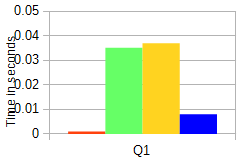
\includegraphics[width=0.3\textwidth]{img/result/1/11}
			%\caption{R-tree structure}
			\label{fig:queries-1}
		}
		\centering
		\subfloat[]{
			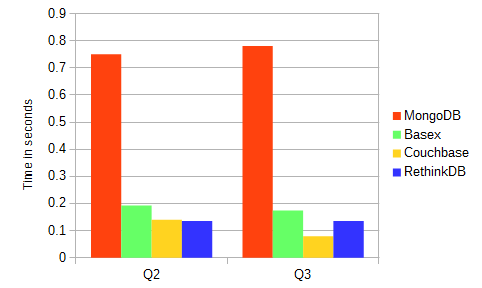
\includegraphics[width=0.6\textwidth]{img/result/1/2-3}
			%\caption{R-tree}
			\label{fig:queries-2-3}
		}\\
		\centering
		\subfloat[]{
			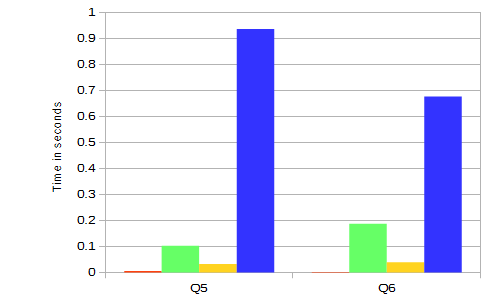
\includegraphics[width=0.5\textwidth]{img/result/1/5-6-2}
			%\caption{R-tree}
			\label{fig:queries-5-6}
		}
		\caption{XMark simple queries}
		\label{fig:query-result}
\end{figure}

 \begin{figure}[H]
		\centering
		\subfloat[]{
			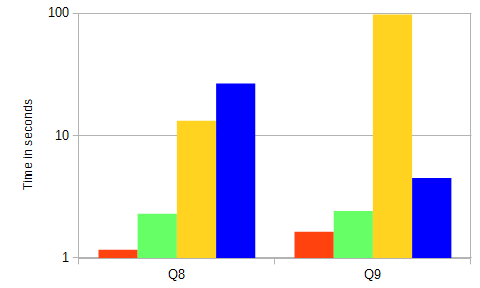
\includegraphics[width=0.5\textwidth]{img/result/1/join-queries-8-9}
			%\caption{R-tree}
			\label{fig:queries-8-9}
		}
		\centering
		\subfloat[]{
			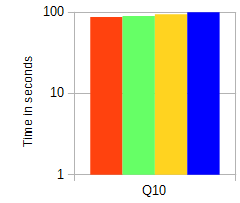
\includegraphics[width=0.3\textwidth]{img/result/1/join-queries-10}
			%\caption{R-tree}
			\label{fig:queries-10}
		}\\
		\centering
		\subfloat[]{
			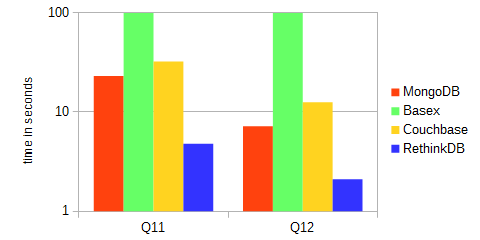
\includegraphics[width=0.8\textwidth]{img/result/1/join-queries-11-12}
			%\caption{R-tree}
			\label{fig:queries-11-12}
		}
		
		\caption{XMark Join Queries.}
		\label{fig:query-result-2}
	\end{figure}
	
\begin{figure}[H]
		\centering
		\subfloat[]{
			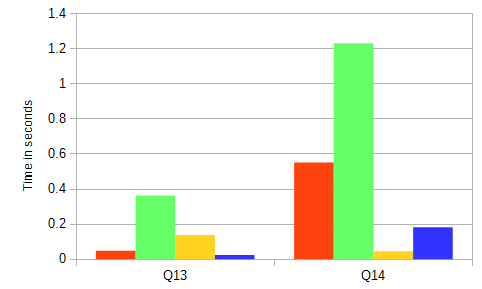
\includegraphics[width=0.4\textwidth]{img/result/1/13-14}
			%\caption{R-tree}
			\label{fig:queries-13-14}
		}
		\centering
		\subfloat[]{
			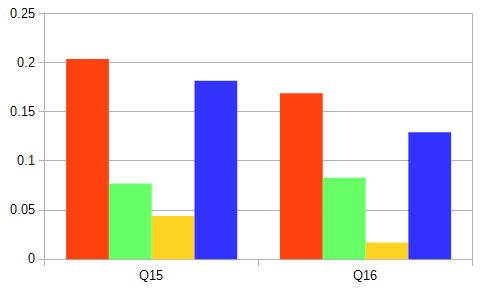
\includegraphics[width=0.4\textwidth]{img/result/1/15-16}
			%\caption{R-tree}
			\label{fig:queries-15-16}
		}\\
		\centering
		\subfloat[]{
			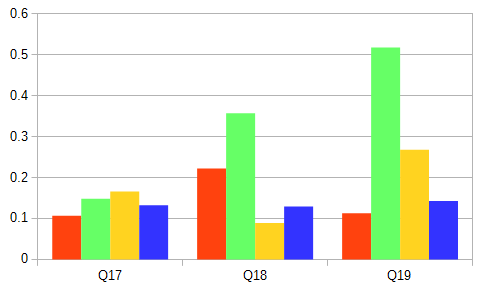
\includegraphics[width=0.5\textwidth]{img/result/1/17-18-19}
			%\caption{R-tree}
			\label{fig:queries-17-19}
		}
		\centering
		\subfloat[]{
			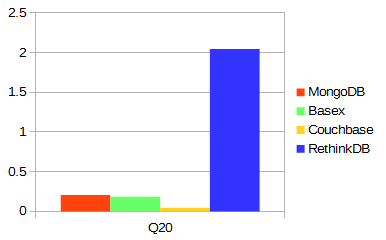
\includegraphics[width=0.4\textwidth]{img/result/1/20}
			%\caption{R-tree}
			\label{fig:queries-20}
		}
		\caption{XMark Advanced Queries.}
		\label{fig:query-result-3}
	\end{figure}
 
 \begin{comment}
  \begin{figure}[H]
		\centering
		\subfloat[XMark Queries No. 1 to 7]{
			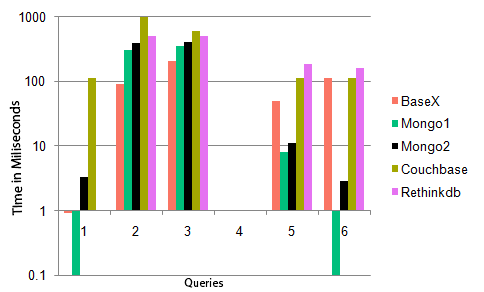
\includegraphics[width=0.3\textwidth]{img/result/1-6}
			%\caption{R-tree structure}
			\label{fig:queries-1-7}
		}
		\centering
		\subfloat[Join Queries (No. 8 to 12)]{
			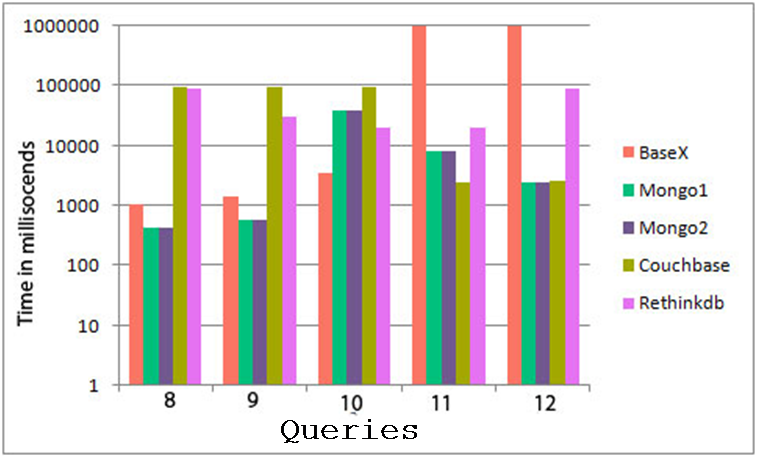
\includegraphics[width=0.5\textwidth]{img/result/8-12}
			%\caption{R-tree}
			\label{fig:queries-8-13}
		}
		
		\centering
		\subfloat[Queries 13 to 20]{
			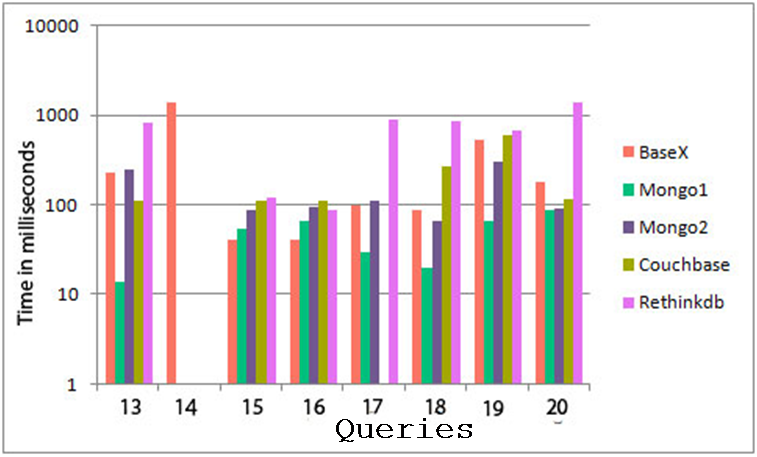
\includegraphics[width=0.44\textwidth]{img/result/13-20}
			%\caption{R-tree}
			\label{fig:queries-13-20}
		}
		\caption{XMark Queries time in XML and NoSQL databases(Mongo1: Mongodb shell, mongo2:through application)}
		\label{fig:query-result}
		
	\end{figure}
\end{comment}
   \subsection{Summary}
	\section{Discussion}
	\section{Conclusion}\label{conc}
	The goal of this thesis was to investigate and analyze the conversion of data from XML database to NoSQL databases. Both types of databases process data of flexible structure. We specifically focused on BaseX, a native XML database, and three document-oriented NoSQL databases: MongoDB, Couchbase and RethinkDB. 

We defined the different data models for each of the NoSQL databases based on the XML database for query and benchmarking purposes. The architecture, query model and indexing mechanism of these databases have been studied and examined. Query plans of the native XML database BaseX were investigated with regard to index optimizations. In contrast, NoSQL databases store data in JSON format. The problems in translating XML to JSON were analyzed. Based on the XMark dataset, some algorithms were defined to convert XML to JSON.

The XQuery expressions of the standard XML benchmarking project XMark were rewritten for the NoSQL databases and their data model. We tested and analyzed the performance of all systems. The experiment was done by running different types and numbers of queries with variable database sizes.
\par
Although BaseX, MongoDB, Couchbase and RethinkDB have been designed to store and process unstructured and semi-structure-data, they are comparatively different systems with regard to the underlying data model, query technique and indexing mechanism.

In the performance results, it was shown that the secondary indexes of NoSQL databases could be utilized to speed up many of the rewritten queries. Even though the execution time of queries with deep child axes seems to be comparable, the results produced by the NoSQL databases were not quite as good as for the XPath-based processor BaseX. Some queries cannot be compared in case of performance as the purpose of different like in Q14.

XQuery is a powerful functional language for XML databases. Most of the NoSQL databases only support basic query operations. MongoDB has a some more query features compared to Couchbase. ReQL, the query language of RethinkDB is the most advanced among the NoSQL databases.

\par
%NoSQL databases are designed to handle a small size of large numbers of documents. They cannot process a huge block of data, but if forced to do so the performance will reduce. The XML databases process a very large size of XML documents. NoSQL database is suited better for an application with massive updates,  because the write operation is atomic in a single document. On the other hand, XML database is best suited for the application that has a large size of documents but fewer write operations.
%If the application has large size of documents but less write operations,  XML database suited better. 

%Even though both of these systems are designed to handle the data that are do not have pre-defined model or  


%In this thesis, we have discussed about the different aspect of semi-structure data and the way they managened. JSON and XML are the most common format to store and transfer the data. Even though their objective are similar, they are incompativale to each other. 
%An algorithms on the besis of XMark dataset was defined to convert XML to JSON.  



%The project was an investigation and comparison of two new database management system  XML database and NoSQL database.  In this project, we have investigated two very famous and most used data format. 
	\section{Future Work}\label{s.future}
	\begin{appendices}
	   	\chapter{XMARK Queries}\label{appendices-queries}
		\section{MongoDB}\label{mongodb-query-list}
			\label{xmark-queries-mongodb}
\begin{enumerate}[label=Q\arabic*.]
	\item %1
	\begin{lstlisting}[language=JSON,   basicstyle=\scriptsize]
		db.people.find({_id:"person0"},{_id:0,"name":1});
	\end{lstlisting}
	
	\item %2
	\begin{lstlisting}[language=JSON,  basicstyle=\scriptsize]
	db.open_auctions.aggregate([
		{$project:{_id:1,bidder:"$bidder"}},
		{ $unwind: "$bidder"},
		{$group:{_id:"$_id",increase:{$first:"$bidder.increase"}}},
		{$sort:{_id:1}},
		{ $unwind: "$increase"},
		{$project:{_id:0,increase:1}}
	])
	\end{lstlisting}
	
    \item %3
	\begin{lstlisting}[language=JSON,   basicstyle=\scriptsize]
	   db.open_auctions.aggregate([
		{ $unwind: "$bidder"},
		{$group:{_id:"$_id",first:{$first:"$bidder.increase"},last:{$last:"$bidder.increase"}}},
		{$unwind:"$first"},
		{$unwind:"$last"},
		{$project:{_id:1,first:1,last:1,diff:{$gte:["$last",{$multiply:["$first",2]}]}}},
		{$match:{diff:true}},
		{$sort:{_id:1}},
		{$project:{_id:0,increase:{first:"$first",last:"$last"}}}
	   ])
	\end{lstlisting}
	
	
    \item %4
	\begin{lstlisting}[language=JSON,   basicstyle=\scriptsize]
	   []
	\end{lstlisting}
	
	
    \item %5
	\begin{lstlisting}[language=JSON,   basicstyle=\scriptsize]
	   db.closed_auctions.find({price:{$gte:40}}).count()
	\end{lstlisting}
	
    \item %6
	\begin{lstlisting}[language=JSON,   basicstyle=\scriptsize]
	   db.regions.find().count()
	\end{lstlisting}
	
	
    \item %7
	\begin{lstlisting}[language=JSON,   basicstyle=\scriptsize]
	   []
	\end{lstlisting}
	
	
    \item %8
	\begin{lstlisting}[language=JSON,   basicstyle=\scriptsize]
	   function q8() {
        	var ids = new Array();
        	var name = new Array();
        	var closed = new Array();
        	var i=0;
        	db.people.find({},{name:1}).forEach(function(people){
        		ids[i] = people._id;
        		name[ids[i]] = people.name;
        		//closed[ids[i]] = {name:people.name,count:0};
        		i++;
        	});
        	var closed_auc = db.closed_auctions.aggregate([
        		{$project:{_id:1,person:"$buyer.person"}},
        		//{$match:{person:{$in:["person12124","person12883"]}}},
        		{$match:{person:{$in:ids}}},
        		{$group:{_id:"$person",count:{$sum:1}}},
        		{$sort:{count:-1}},
        		{$project:{person:"$_id",count:1,_id:0}}
        	]);
        	if(closed_auc) {
        		var i=0
        		while(closed_auc.hasNext()){
        			var auc = closed_auc.next();
        			var id = auc.person;
        			closed[i] = {"name":name[id],"count":auc.count}
        			name[id] = 0;
        			i++;
        			//printjson(name.indexOf(id));
        		}
        		
        	}/**/
        	var len = closed.length ;
        	var j = 0;
        	for(var i=0; i < ids.length; i++) {
        		if(name[ids[i]] !== 0) {
        		//printjson(i);
        		closed[len+j]	= {"name":name[ids[i]],"count":0};
        		j++;
        		}
        	}
        	//printjson("Execution Time" + end-start);
        	return closed;
        	
        }
	\end{lstlisting}
	
	
    \item %9
	\begin{lstlisting}[language=JSON,   basicstyle=\scriptsize]
	   
	\end{lstlisting}
	
	
    \item %10
	\begin{lstlisting}[language=JSON,   basicstyle=\scriptsize]
	//helper function for Q10.
    var getProfileByCategory = function(catId){
    		var prof = new Array();
    		var i = 0;
    		db.people.find(
    		{"profile.interest":{$exists:true},"profile.interest":{"$elemMatch": {category:catId}}},
    		{name:1, profile:1,address:1}
    		).forEach(function(p){
    			if(!p.address) {
    				p.address = {};
    			}
    			var c = function (value){return ((value) && (typeof value !== "undefined")) ? value : "";}; 
    			prof[i] = {
                          personne: {
                            statistiques: {
                              sexe: c(p.profile.gender),
                              age: c(p.profile.gender),
                              education: c(p.profile.education),
                              revenu: c(p.profile.income)
                            },
                            coordonnees: {
                              nom: p.name,
                              rue: (c(p.address)&&c(p.address.street)),
                              ville: c(p.address.city),
                              pays: c(p.address.country),
                              reseau: {
                                courrier: c(p.emailaddress),
                                pagePerso: c(p.homepage)
                              }
                            },
                            cartePaiement: c(p.creditcard)
                          }
                        }
                            			
    			})
    		return prof;
    		};
    		
    		
	   function q10() {
        	var debugId = "person3"
        	var ids = new Array();
        	var i = 0;
        	var allcategories = new Array();
        	db.people.aggregate([
        	{$match:{"profile.interest":{$exists:true}}},
        	{$project:{_id:1, interest:"$profile.interest"}},
        	{$unwind:"$interest"},
        	{$group:{_id:"$interest.category"}},
        	{$project:{_id:0, category:"$_id"}}
        	]).forEach(function(people){
        		var catId = people.category;
        		ids[i] = {categorie:{id:catId,profile:getProfileByCategory(catId)}}
        		i++;
        	});
        	return ids;
        }
	\end{lstlisting}
	
	
    \item %11
	\begin{lstlisting}[language=JSON,   basicstyle=\scriptsize]
	  function q11() {
    	var start = new Date().getTime();
    	var debugId = "person3"
    	var ids = new Array();
    	var open_auc = function(initial){
    		return db.open_auctions.find({initial:{$lt:initial}},{_id:1}).count();
    	}
    	
    	var i=0;
    	db.people.find({},{_id:1, name:1,"profile.income":1}).forEach(function(people){
    		var income = ((people.profile) && people.profile.income)? people.profile.income/5000:0;
    		ids[i] = {item:{name: people.name,id:people._id,count:open_auc(income)}};
    		i++;
    	});
    	return ids;
        }
	\end{lstlisting}
	
	
    \item %12
	\begin{lstlisting}[language=JSON,   basicstyle=\scriptsize]
	   function q12() {
    	var debugId = "person3"
    	var ids = new Array();
    	var open_auc = function(initial){
    		return db.open_auctions.find({initial:{$lt:initial}},{_id:1}).count();
    	}
    	var i=0;
    	db.people.find({"profile.income":{$exists:true}, "profile.income":{$gt:50000}},{_id:1, name:1,"profile.income":1}).forEach(function(people){
    		var income = ((people.profile) && people.profile.income)? people.profile.income/5000:0;
    		ids[i] = {item:{name: people.name,id:people._id,count:open_auc(income)}};
    		i++;
    	});
    	return ids;

    }
	\end{lstlisting}
	
	\item %13
	\begin{lstlisting}[language=JSON,   basicstyle=\scriptsize]
	    db.regions.find(
		{regions:"australia"},
		{_id:0,name:1,description:1}
        )
	\end{lstlisting}
	
    \item %14
	\begin{lstlisting}[language=JSON,   basicstyle=\scriptsize]
	  db.regions.aggregate([
		{$match:{$text:{$search:"gold"}}},
		{$group:{_id:"$_id"}},
		{$group:{_id:null,count:{$sum:1}}},
		{$project:{_id:0,count:1}}
	])
	\end{lstlisting}
	
    \item %15
	\begin{lstlisting}[language=JSON,   basicstyle=\scriptsize]
	 db.closed_auctions.aggregate([
		{$project:{_id:1,parlist:"$annotation.description.parlist"}},
		{ $unwind: "$parlist"},
		{ $unwind: "$parlist.listitem.parlist"},
		{$project:{_id:1,text:"$parlist.listitem.parlist.listitem.text"}},
		{$match:{$or:[{"text.emph.keyword":{$exists:true}},{"text.emph.keyword.childtext":{$exists:true}},{"text.emph.keyword.child":{$exists:true}}]}},
		{$project:{_id:0,text:"$text.emph.keyword"}}
	])
	\end{lstlisting}
	
    \item %16
	\begin{lstlisting}[language=JSON,   basicstyle=\scriptsize]
	  db.closed_auctions.aggregate([
		{$project:{_id:1,parlist:"$annotation.description.parlist",person:"$seller.person"}},
		{ $unwind: "$parlist"},
		{ $unwind: "$parlist.listitem.parlist"},
		{$project:{_id:1,text:"$parlist.listitem.parlist.listitem.text",person:1}},
		{$match:{"text.emph.keyword":{$exists:true}}},
		{$project:{_id:0,"person.id":"$person"}}
	])
	\end{lstlisting}	

    \item %17
	\begin{lstlisting}[language=JSON,   basicstyle=\scriptsize]
	  db.people.find({homepage:{$exists:false}},{_id:0,person:"$name"})
	])
	\end{lstlisting}	

    \item %18
	\begin{lstlisting}[language=JSON,   basicstyle=\scriptsize]
	  db.open_auctions.aggregate([{$match:{reserve:{$exists:true}}},
		{$project:{_id:0,reserve:{$multiply:["$reserve",2.20371]}}}])
	\end{lstlisting}	

    \item %19
	\begin{lstlisting}[language=JSON,   basicstyle=\scriptsize]
	  db.regions.aggregate([{$sort:{location:1}},
		{$project:{_id:0,"item.name":"$name","item.location":"$location"}}])
	\end{lstlisting}	
    
    \item %20
	\begin{lstlisting}[language=JSON,   basicstyle=\scriptsize]
	  db.people.aggregate([
		{$project:{_id:1,p:"$profile.income"}},
		{$project:{_id:1,con:
			{$cond:[
			  {$gt:["$p",100000]},"preferred",
			  {$cond:[{ $and: [{$lt:["$p", 100000] }, {$gte:["$p", 30000] }] },"standard",
		{$cond:[{$and:[{$lt:["$p",30000]},{$gt:["$p",0]}]},"challange","na"]}
		]}
		]}
		}},
		{$group:{_id:"$con",sum:{$sum:1}}},
		{$project:{_id:1,sum:1}}])
	\end{lstlisting}
\end{enumerate}
\noindent\makebox[\linewidth]{\rule{\paperwidth}{0.4pt}}
\begin{lstlisting}[language=JSON,   basicstyle=\scriptsize, label=mongodb-xmark-index, caption=Secondary indexes in MongoDB's XMark data]
	  db.open_auctions.ensureIndex({
		initial:1
	})
	db.open_auctions.ensureIndex({
		bidder:1
	})
	db.open_auctions.ensureIndex({
		"bidder.increase":1
	})
	
	db.regions.ensureIndex({
		name:1,
		location:1
	})
	db.regions.ensureIndex({
		regions:1
	})
	db.regions.ensureIndex({
		location:1
	})
	db.regions.ensureIndex([
                   { "$**": "text" },
                   { name: "TextIndex" }
                         ])
	db.people.ensureIndex({
		"people.interest":1
	})

	db.closed_auctions.ensureIndex({
		"buyer.person":1
	});
	db.closed_auctions.ensureIndex({price:1})
	\end{lstlisting}

		\section{RethinkDB}\label{rethinkdb-query-list}
				\label{xmark-queries-rethindb}
\begin{enumerate}[label=Q\arabic*.]
	\item %1
	
	\begin{lstlisting}[language=JSON, basicstyle=\scriptsize]
		r.table("people").get("person0")("name")
	\end{lstlisting}

	\item %2
	\begin{lstlisting}[language=JSON, basicstyle=\scriptsize]
	r.table("open_auctions").map(function(doc) {return {increase:doc("bidder").nth(0)("increase").nth(0).default("")}})
	
	\end{lstlisting}
	
    \item %3
	\begin{lstlisting}[language=JSON, basicstyle=\scriptsize]
	  r.table("open_auctions").hasFields("bidder").filter(
	                r.row("bidder").nth(0)("increase").nth(0).mul(2).le(r.row("bidder").nth(r.row("bidder").count().sub(1))("increase").nth(0))
	              ).map(function(doc){
	                var last = doc("bidder").count().sub(1);
	                return {increase:{first:doc("bidder").nth(0)("increase").nth(0), last:doc("bidder").nth(last)("increase").nth(0)} }
	              })
	\end{lstlisting}
	
	
    \item %4
	\begin{lstlisting}[language=JSON, basicstyle=\scriptsize]
	   
	\end{lstlisting}
	
	
    \item %5
	\begin{lstlisting}[language=JSON, basicstyle=\scriptsize]
	   r.table("closed_auctions").count(function(f){
	                 return f("price").default(0).gt(40)
	               })
	\end{lstlisting}
	
    \item %6
	\begin{lstlisting}[language=JSON, basicstyle=\scriptsize]
	   r.table("regions").count()
	\end{lstlisting}
	
	
    \item %7
	\begin{lstlisting}[language=JSON, basicstyle=\scriptsize]
	   
	\end{lstlisting}
	
	
    \item %8
	\begin{lstlisting}[language=JSON, basicstyle=\scriptsize]
	  r.table("people").map(function(d){
	                var x = r.table("closed_auctions").getAll(d("id"),{index:"buyer_person"}).count();
	                return {person:d("name"),value:x}
	              }).orderBy(r.desc("value")).map({item:r.row})
	\end{lstlisting}
	
	
    \item %9
	\begin{lstlisting}[language=JSON, basicstyle=\scriptsize]
	   r.table("regions").getAll("europe",{index:"regions"}).eqJoin("id",r.table("closed_auctions"),{index:"closed_itemref_item"}).map({
	                 name:r.row("left")("name"), id:r.row("left")("id"),
	               })
	\end{lstlisting}
	
	
    \item %10
    
	\begin{lstlisting}[language=JSON, basicstyle=\scriptsize]
	   r.table("people")("profile")("interest").concatMap(function(f){return f}).distinct()
	                 .merge(function(category){
	                   return {
	                     d:
	                    r.table("people").filter(function(d){
	                 return d("profile")("interest").contains(function(e){
	                   return e("category").eq(category("category"))})}).map(function(profile){
	                      return {
	                        personne:{
	                          statistiques:{
	                            sexe:profile("profile")("gender").default(""),
	                            age:profile("profile")("age").default(""),
	                            education:profile("profile")("education").default(""),
	                            revenu:profile("profile")("income").default("")
	                          },
	                          coordonnees: {
	                            nom:profile("name"),
	                            rue: profile("address")("street").default(""),
	                            ville:profile("address")("city").default(""),
	                            pays:profile("address")("country").default(""),
	                            reseau:{
	                            courrier:profile("emailaddress").default(""),
	                            pagePerso:profile("homepage").default("")
	                          }
	                          },
	                        cartePaiement:profile("creditcard").default("")
	   
	                        }
	                      }
	                    }).coerceTo('array')
	                   }
	                 })
	\end{lstlisting}
	
	
    \item %11
    
	\begin{lstlisting}[language=JSON, basicstyle=\scriptsize]
	 r.table("people").pluck("id",{profile:{income:true}})
	               .map(function(f){
	                 var i = f("profile")("income").default(0).div(5000);
	                 return {
	                   id:f("id"),
	                   item:r.table("open_auctions").filter(function(m){
	                  return  m("initial").default(0).lt(i)
	                     }).count()
	                  }
	          })
	\end{lstlisting}
	
	
    \item %12
	\begin{lstlisting}[language=JSON, basicstyle=\scriptsize]
	   r.table("people").filter(function(f){return f("profile")("income").default(0).gt(50000)})
	                 .map(function(f){
	                 return {
	                   id:f("id"),
	                   item:r.table("open_auctions").count(function(x){
	                     return f("profile")("income").default(0).gt(x("initial").default(0).mul(5000))
	                   })
	                 }
	               })
	\end{lstlisting}
	
	
    \item %13
	\begin{lstlisting}[language=JSON, basicstyle=\scriptsize]
	   r.table("regions").getAll("australia",{index:"regions"}).map({item:{name:r.row("name"),description:r.row("description")}})
	\end{lstlisting}
	
    \item %14
	\begin{lstlisting}[language=JSON, basicstyle=\scriptsize]
	 	r.table("regions").filter(function(doc) {
	 	    return doc('description').coerceTo("STRING").match("gold")
	 	    })('name') 
	\end{lstlisting}	

    \item %15
	\begin{lstlisting}[language=JSON, basicstyle=\scriptsize]
	 r.table("closed_auctions")("annotation")("description")("parlist").concatMap(function(f){
	           return f('listitem')('parlist')
	         }).concatMap(function(f){return f('listitem').hasFields({text:{emph:{keyword:true}}})}).map(function(f){
	           return {"text":f('text')('emph')('keyword')}
	         })
	\end{lstlisting}	

    \item %16
	\begin{lstlisting}[language=JSON, basicstyle=\scriptsize]
	  r.table("closed_auctions").hasFields({annotation:{description:{parlist:true}}})
	              ("annotation")("description").concatMap(r.row("parlist")).hasFields({listitem:{parlist:true}})("listitem").concatMap(r.row("parlist")).hasFields({listitem:{text:{emph:{keyword:true}}}})
	\end{lstlisting}	

    
    \item %17
	\begin{lstlisting}[language=JSON, basicstyle=\scriptsize]
	  r.table("people").filter(function(d){return d.hasFields("homepage").not()}).map({person:{name:r.row("name")}})
	\end{lstlisting}	

    \item %18
	\begin{lstlisting}[language=JSON, basicstyle=\scriptsize]
	  r.table("open_auctions").hasFields("reserve").map(r.row("reserve").mul(2.20371))
	\end{lstlisting}	

    \item %19
	\begin{lstlisting}[language=JSON, basicstyle=\scriptsize]
	  r.table("regions").orderBy({index:"location"}).pluck("location","name").map(function(f){
	    return {item:{name:f("name"),location:f("location")}}
	  })
	\end{lstlisting}
	
    \item %20
	\begin{lstlisting}[language=JSON, basicstyle=\scriptsize]
	  r.table("people").map(function(doc){return {income:doc("profile")("income").default(0)}})
	            .map({
	             preferred:r.branch(r.row("income").ge(100000),'preferred',0),
	            standard:r.branch(r.row("income").le(100000).and(
	              r.row("income").ge(30000)
	            ),'standard',0),
	            challenge:r.branch(r.row("income").le(30000).and(
	              r.row("income").gt(0)
	            ),'challenge',0),
	            na:r.branch(r.row("income").le(0),'na',0)
	          }).group('preferred','standard','challenge','na').count()
	\end{lstlisting}

\end{enumerate}

		\section{Couchbase}\label{couchbase-query-list}
				\label{xmark-queries-couchbase}
\begin{enumerate}[label=Q\arabic*.]
	\item %1
	\begin{lstlisting}[language=JSON, basicstyle=\scriptsize]
			function (doc, meta) {
			   if(doc.doctype && doc.doctype=="people" && doc.id=="person0"){
				emit(doc.name);	   
			    }
			  
			}
		\end{lstlisting}

	\item %2
	\begin{lstlisting}[language=JSON, basicstyle=\scriptsize]
	function (doc, meta) {
	   if(doc.doctype && doc.doctype=="open_auctions"){
	     if(doc.bidder){
	     	var first = doc.bidder[0];
	       for(var i=0; i<first.length;i++) {
	         if(first[i].increase) {
	           var increase = first[i].increase;
	           //emit(doc.id,increase)
	           emit("increase",increase)
	           break;
	         }
	       }
	     } else {
	     	      emit("increase",null)
	     }
	   }
	}
	\end{lstlisting}
	
    \item %3
	\begin{lstlisting}[language=JSON, basicstyle=\scriptsize]
	  function (doc, meta) {
       if(doc.doctype && doc.doctype=="open_auctions" 
            && doc.bidder) {
         	var first = doc.bidder[0];
           	var last = doc.bidder[(doc.bidder.length - 1)];
            var increaseFirst = 0;
            var increaseLast = 0;
           
           for(var i=0; i<first.length;i++) {
             if(first[i].increase) {
               increaseFirst = first[i].increase;
               break;
             }
           }
           for(var i=0; i<last.length;i++) {
             if(last[i].increase) {
               increaseLast = last[i].increase;
               break;
             }
           }
           if(increaseFirst && increaseLast) {
             if(increaseFirst * 2 <= increaseLast ){
    	   emit({increase:{first:increaseFirst,last:increaseLast,id:doc.id}});
             }
           } 
       }
    }
	\end{lstlisting}
	
	
    \item %4
	\par
	
	
    \item %5
	\begin{lstlisting}[language=JSON, basicstyle=\scriptsize]
	map:
	   function (doc, meta) {
	      if(doc.doctype && doc.doctype=="closed_auctions"){
	        if(doc.price){
	          if(doc.price >= 40) {
	            emit(doc.id,doc.price)
	          }
	       }
	    }
	  }
	  reduce: 
	    _count
	\end{lstlisting}
	
    \item %6
	\begin{lstlisting}[language=JSON, basicstyle=\scriptsize]
	  map:
	  function (doc, meta) {
	     if(doc.doctype && doc.doctype=="regions"){
	         emit(doc.id,null)
	      }
	  }
	  
	  reduce: 
	  _count
	\end{lstlisting}
	
	
    \item %7
    \par
	
	
    \item %8
	\begin{lstlisting}[language=JSON, basicstyle=\scriptsize]
	View1: person_info
	map:
	function (doc, meta) {
      if(doc.doctype && doc.doctype=="people")
      emit(meta.id, doc.name);
    }
    
    View 2: Aggregate
    map:
    
    function (doc, meta) {
      if(doc.doctype=="people"){
        emit(meta.id,0);
          } else if (doc.doctype=="closed_auctions"){
            if(doc.buyer.person){
              emit(doc.buyer.person,1);
             }
          }
    }
    
    reduce: 
        _sum
	\end{lstlisting}
	
	
    \item %9
\par
	
	
    \item %10
	\begin{lstlisting}[language=JSON, basicstyle=\scriptsize]
	  View 1: 
	 map:
	 function (doc, meta) {
      if(doc.doctype && doc.doctype=="people" 
      && doc.profile && doc.profile.interest){
        var interest = doc.profile.interest;
            for(i=0; i < interest.length; i++) {
          if(interest[i] && interest[i].category) {
            emit(interest[i].category, meta.id) 
          }
        }
      }
    }

reduce:
    function(keys, values, rereduce) {
      return values
    }
query:
    group_level:1
	   
    View 2: 
    Map: 
    
   function (doc, meta) {
  if(doc.doctype && doc.doctype=="people" && doc.profile && doc.profile.interest){
  
    var profile = doc.profile;
    var p = {statistiques:{sexe:"",age:"",education:"",revenu:""},
              coordonnees:{ nom:doc.name,rue:doc.address.street,ville:doc.address.city,
                           pays:doc.address.country,reseau:{courrier:doc.emailaddress
                                                            ,pagePerso:doc.homepage}
                         },
             cartePaiement:""
            
            };
    
    for(var j in profile){
      if(j != "interest"){
       	p[j] = profile[j];
        switch(j){
          case 'gender':
            p.statistiques.sexe = profile[j];  
          break;
          case 'age':
            p.statistiques.age = profile[j];  
          break;
          case 'education':
            p.statistiques.education = profile[j];  
          break;
          case 'income':
            p.statistiques.revenu = profile[j];  
          break;
         }
      }
      
    }
   emit(meta.id,p) 
  
  }
}
	\end{lstlisting}
	
	
    \item %11
	\begin{lstlisting}[language=JSON, basicstyle=\scriptsize]
	view 1: 
	map:
	
	  function (doc, meta) {
      if(doc.doctype && doc.doctype=='open_auctions') {
        var initial = (doc.initial)?doc.initial :0;
      	emit(meta.id, initial*5000);	
      }
    }
    view 2: 
    function (doc, meta) {
      if(doc.doctype && doc.doctype=="people"){
        var income = (doc.profile && doc.profile.income)? doc.profile.income :0;
        emit(doc.name, income);
      }
    }
	\end{lstlisting}
	
	\item %12
	\begin{lstlisting}[language=JSON, basicstyle=\scriptsize]
	view 1: 
	map:
	
	  function (doc, meta) {
      if(doc.doctype && doc.doctype=='open_auctions') {
        var initial = (doc.initial)?doc.initial :0;
      	emit(meta.id, initial*5000);	
      }
    }
    
    View 2: 
    
   function (doc, meta) {
    if(doc.doctype && doc.doctype=="people"){
    var income = (doc.profile && doc.profile.income)? doc.profile.income :0;
    if(income > 5000)
    emit(doc.name, income);
    }
  }
	\end{lstlisting}
	
	
    \item %13
	\begin{lstlisting}[language=JSON, basicstyle=\scriptsize]
	   function (doc, meta) {
	     if(doc.doctype && doc.doctype == "regions" 
	     && doc.regions && doc.regions=="australia"){
	       if(doc.description){
	         emit("item",{name:doc.name, description:doc.description})
	       
	       }
	     }
	   }
	\end{lstlisting}
	
    \item %14
	\begin{lstlisting}[language=JSON, basicstyle=\scriptsize]
		//don't supprt full text search
	 	function (doc, meta) {
	 	  if(doc.doctype && doc.doctype=="regions"){
	 	   
	 	    if(doc.description){
	 	       var desc = JSON.stringify(doc.description);
	 	      if(desc.indexOf("gold") !== -1)
	 	       emit(meta.id, doc.name);
	 	   }
	 	  }
	 	}
	\end{lstlisting}	

    \item %15
	\begin{lstlisting}[language=JSON, basicstyle=\scriptsize]
	 function (doc, meta) {
	   if(doc.doctype=="closed_auctions"){
	     var p1 = doc.annotation.description.parlist;
	     if(p1){
	       for(var i=0;i<p1.length;i++){
	       	var p2 = p1[i].listitem.parlist;
	         if(p2) {
	           for(var j=0;j<p2.length;j++){
	             
	             if(p2[j].listitem && p2[j].listitem.text && p2[j].listitem.text.emph && p2[j].listitem.text.emph.keyword){
	             	var keyword = p2[j].listitem.text.emph.keyword;
	               emit("text", keyword);   
	             }
	           }
	         }
	       }
	     }
	   }
	 }
	\end{lstlisting}	

    \item %16
	\begin{lstlisting}[language=JSON, basicstyle=\scriptsize]
	 function (doc, meta) {
	   if(doc.doctype=="closed_auctions"){
	     var p1 = doc.annotation.description.parlist;
	     if(p1){
	       var person = (doc.seller.person)?doc.seller.person:0;
	       for(var i=0;i<p1.length;i++){
	       	var p2 = p1[i].listitem.parlist;
	         if(p2) {
	           for(var j=0;j<p2.length;j++){
	             
	             if(p2[j].listitem && p2[j].listitem.text && p2[j].listitem.text.emph && p2[j].listitem.text.emph.keyword){
	             	var keyword = p2[j].listitem.text.emph.keyword;
	               if(person){
	               	emit("person", {id:person});     
	               }
	               
	             }
	           }
	         }
	       }
	     }
	   }
	 }
	\end{lstlisting}	

    
    \item %17
	\begin{lstlisting}[language=JSON, basicstyle=\scriptsize]
	  function (doc, meta) {
	    if(doc.doctype=="people"){
	      if(!doc.homepage && doc.name){
	        emit("name",doc.name)
	      } 
	    }
	  }
	\end{lstlisting}	

    \item %18
	\begin{lstlisting}[language=JSON, basicstyle=\scriptsize]
	  function (doc, meta) {
      if(doc.doctype=="open_auctions"){
        
        if(doc.reserve){
          var reserve = function(val){ return parseFloat(val) * 2.20371 }
          emit(reserve(doc.reserve))
        } 
      }
    }
	\end{lstlisting}	

    \item %19
	\begin{lstlisting}[language=JSON, basicstyle=\scriptsize]
	  function (doc, meta) {
	    if(doc.doctype=="regions" && doc.name){
	      var location = (doc.location)?doc.location:"";
	      emit(location,{item:{name:doc.name,location:location}});
	    }
	  }
	  })
	\end{lstlisting}	
    \item %20
	\begin{lstlisting}[language=JSON, basicstyle=\scriptsize]
	  map:
	  function (doc, meta) {
      if(doc.doctype=="people"){ 
        var income = (doc.profile && doc.profile.income)? doc.profile.income : 0;
         if(income >= 100000 ){
      	 emit("preferred",1);
        }else if(income < 100000 && 
                 income >= 30000) {
          emit("standard",1);
        }else if(income < 30000 &&
             income > 0 ){
          emit("challenge",1);
        } else {
         emit("na",1);
        }    
      }
    }

	  reduce:
	    _sum
	 
	 query:
	    group_level=1
	\end{lstlisting}

\end{enumerate}

				\newpage
\begin{center}
\begin{table}[ht]
\tiny
\label{basex-query-result-table}
\caption{BaseX}
\begin{tabular}{|c|c|c|c|c|c|c|c|c|c|c| } 
    &  1 & 2 & 3 & 4 & 5 & 6 & 7 & 8 & 9 & 10 \\
 \hline
0001 & 0.002 & 0.003 & 0.005 & 0.0382 & 0.004 & 0.004 & 0.0377 & 0.007 & 0.008 & 0.012	\\
001 & 0.003 & 0.006 & 0.006 & 0.0411 & 0.005 & 0.006 & 0.0433 & 0.01 & 0.012 & 0.025	\\
01 & 0.004 & 0.017 & 0.057 & 0.01 & 0.025 & 0.016 & 0.1552 & 0.067 & 0.098 & 0.943	\\
1 & 0.003 & 0.068 & 0.1341 & 0 & 0.045 & 0.1876 & 0.9612 & 0.714 & 1.118 & 79.3573	\\
5 & 0.0181 & 0.6882 & 0.7167 & 0.5554 & 0.3297 & 0.5373 & 4.5321 & 12.9726 & 18.1868 & 2572.0186	\\
10 & 0.004 & 1.6552 & 1.6249 & 1.1203 & 0.7955 & 1.4824 & 9.4888 & 29.3343 & 37.493 & 127200	\\
20 & 0.004 & 3.4515 & 10.1975 & 3.7436 & 1.5508 & 3.6199 & 27.5222 & 59.1221 & 115.4997 & 10000	\\
\end{tabular}
\begin{tabular}{|c|c|c|c|c|c|c|c|c|c|c| } 
Size & 11 & 12 & 13 & 14 & 15 & 16 & 17 & 18 & 19 & 20	\\
\hline
0001 & 0.015 & 0.015 & 0.006 & 0.005 & 0.004 & 0.004 & 0.004 & 0.005 & 0.006 & 0.005	\\
001 & 0.23 & 0.133 & 0.006 & 0.016 & 0.005 & 0.005 & 0.005 & 0.006 & 0.009 & 0.009	\\
01 & 23.58 & 12.54 & 0.033 & 0.174 & 0.009 & 0.008 & 0.012 & 0.14 & 0.042 & 0.038	\\
1 & 2404.1736 & 1283.4839 & 0.3643 & 1.2326 & 0.0773 & 0.083 & 0.1481 & 0.357 & 0.5178 & 0.1857	\\
5 & 24040.1736 & 12830.4839 & 1.6621 & 6.3384 & 0.2622 & 0.203 & 0.5386 & 0.6565 & 2.1216 & 0.9107	\\
10 & 240400 & 128300 & 2.984 & 12.267 & 1.2469 & 0.4025 & 1.1996 & 1.9845 & 5.6113 & 2.4085	\\
20 & 10000 & 10000 & 5.9743 & 26.117 & 2.4337 & 0.794 & 2.6421 & 3.4999 & 63.6597 & 7.2226	\\
\end{tabular}
\end{table}

\begin{table} [ht]
\tiny
\caption{MongoDB With Index}
\label{mongodb-query-result-table}
\begin{tabular}{|c|c|c|c|c|c|c|c|c|c|c| } 
    &  1 & 2 & 3 & 4 & 5 & 6 & 7 & 8 & 9 & 10 \\
 \hline
0001 & 0.001 & 0.002 & 0.004 & 0 & 0.001 & 0.001 & 0 & 0.004 & 0.004 & 0.003	\\
001 & 0.001 & 0.014 & 0.009 & 0 & 0.002 & 0.001 & 0 & 0.012 & 0.021 & 0.047	\\
01 & 0 & 0.079 & 0.079 & 0 & 0.002 & 0.002 & 0 & 0.106 & 0.147 & 1.265	\\
1 & 0.001 & 0.986 & 0.451 & 0 & 0.006 & 0.004 & 0 & 1.172 & 1.645 & 87.251	\\
5 & 0.001 & 4.171 & 4.786 & 0 & 0.028 & 0.003 & 0 & 7.373 & 9.028 & 0	\\
10 & 0.001 & 6.42 & 4.71 & 0 & 0.033 & 0.006 & 0 & 9.367 & 15.002 & 100000	\\
20 & 0.001 & 16.402 & 16.658 & 0 & 0.068 & 0.002 & 0 & 19.42 & 24.336 & 100000	\\

\end{tabular}
\begin{tabular}{|c|c|c|c|c|c|c|c|c|c|c| } 
Size & 11 & 12 & 13 & 14 & 15 & 16 & 17 & 18 & 19 & 20	\\
\hline
0001 & 0.016 & 0.003 & 0.001 & 0.001 & 0.002 & 0.001 & 0.003 & 0.002 & 0.002 & 0.003	\\
001 & 0.177 & 0.045 & 0.004 & 0.004 & 0.008 & 0.003 & 0.004 & 0.006 & 0.003 & 0.008	\\
01 & 1.965 & 0.409 & 0.012 & 0.010 & 0.028 & 0.023 & 0.015 & 0.028 & 0.016 & 0.048	\\
1 & 23.133 & 7.21 & 0.059 & 0.025 & 0.204 & 0.169 & 0.107 & 0.245 & 0.113 & 0.508	\\
5 & 0 & 107.336 & 0.068 & 3.401 & 0.222 & 0.178 & 0.202 & 0.915 & 3.556 & 1.157	\\
10 & 510.781 & 204.499 & 0.047 & 0.055 & 0.212 & 0.14 & 0.192 & 110.01 & 0.202 & 4.885	\\
20 & 100000 & 727.909 & 0.053 & 0.111 & 0.202 & 0.148 & 0.206 & 454.298 & 0.163 & 9.794	\\


\end{tabular}
\end{table}



\begin{table} [ht]
\tiny
\caption{MongoDB Without Index}
\label{mongodb-noindex-query-result-table}
\begin{tabular}{|c|c|c|c|c|c|c|c|c|c|c| } 
    &  1 & 2 & 3 & 4 & 5 & 6 & 7 & 8 & 9 & 10 \\
 \hline
0001 & 0 & 0.003 & 0.003 & 0 & 0 & 0.001 & 0 & 0.01 & 0.011 & 0.004	\\
001 & 0 & 0.008 & 0.006 & 0 & 0 & 0.001 & 0 & 0.031 & 0.028 & 0.046	\\
01 & 0.001 & 0.04 & 0.043 & 0 & 0.002 & 0.001 & 0 & 0.074 & 0.092 & 0.89	\\
1 & 0 & 0.372 & 0.43 & 0 & 0.012 & 0.001 & 0 & 0.52 & 0.801 & 43.082	\\
5 & 0 & 1.885 & 2.14 & 0 & 0.605 & 0.002 & 0 & 2.757 & 6.14 & 1007.605	\\
10 & 0 & 5.243 & 5.552 & 0 & 1.178 & 0.002 & 0 & 7.004 & 12.145 & 0	\\
20 & 0 & 10.677 & 11.423 & 0 & 7.522 & 0.002 & 0 & 23.183 & 67.314 & 0	\\


\end{tabular}
\begin{tabular}{|c|c|c|c|c|c|c|c|c|c|c| } 
Size & 11 & 12 & 13 & 14 & 15 & 16 & 17 & 18 & 19 & 20	\\
\hline
0001 & 0.029 & 0.004 & 0.001 & 0.001 & 0.001 & 0.001 & 0.001 & 0 & 0.002 & 0.001	\\
001 & 0.192 & 0.047 & 0.002 & 0 & 0.003 & 0.001 & 0.002 & 0.001 & 0.004 & 0.002	\\
01 & 4.351 & 0.861 & 0.007 & 0.002 & 0.013 & 0.014 & 0.005 & 0.004 & 0.014 & 0.011	\\
1 & 345.299 & 62.648 & 0.018 & 0.008 & 0.073 & 0.089 & 0.039 & 0.025 & 0.084 & 0.089	\\
5 & 0 & 0 & 0.276 & 2.311 & 0.111 & 0.098 & 0.131 & 0.861 & 2.11 & 0.602	\\
10 & 0 & 0 & 2.066 & 3.998 & 0.135 & 0.074 & 0.156 & 0.854 & 16.448 & 1.36	\\
20 & 0 & 0 & 5.281 & 8.202 & 0.126 & 0.072 & 0.174 & 0.854 & 34.448 & 2.858	\\

\end{tabular}
\end{table}

\begin{table} [ht]
\tiny
\caption{RethinDB}
\label{rethink-query-result-table}
\begin{tabular}{|c|c|c|c|c|c|c|c|c|c|c| } 
    &  01 & 02 & 3 & 4 & 5 & 6 & 7 & 8 & 9 & 10 \\
 \hline
0001 & 0.002 & 0.006 & 0.011 & 0 & 0.026 & 0.010 & 0.1311 & 0.049 & 0.0299 & 0.025	\\
001 & 0.007 & 0.0488 & 0.0886 & 0 & 0.0255 & 0.0162 & 0 & 0.5758 & 0.088 & 0.321	\\
01 & 0.006 & 0.1346 & 0.1381 & 0 & 0.1208 & 0.0624 & 0 & 5.5691 & 0.6748 & 17.23	\\
1 & 0.008 & 0.1356 & 0.1351 & 0 & 0.9371 & 0.4777 & 0 & 26.7616 & 4.5299 & 0\
5 & 0.0046 & 0.129 & 0.1322 & 0 & 1.8228 & 0.1496 & 0 & 133.3807 & 24.342 & 0	\\
10 & 0.0019 & 0.13 & 0.131 & 0 & 3.5512 & 0.4945 & 0 & 239.3042 & 49.38 & 100000	\\
20 & 0.021 & 0.1285 & 0.1324 & 0 & 7.2728 & 0.5985 & 0 & 508.1794 & 98.7042 & 100000	\\

\end{tabular}
\begin{tabular}{|c|c|c|c|c|c|c|c|c|c|c| } 
Size & 11 & 12 & 13 & 14 & 15 & 16 & 17 & 18 & 19 & 20	\\
\hline
0001 & 0.013 & 0.025 & 0.005 & 0.003 & 0.01 & 0.027 & 0.017 & 0.012 & 0.008 & 0.014	\\
001 & 0.1598 & 0.1676 & 0.016 & 0.014 & 0.024 & 0.0278 & 0.0228 & 0.0232 & 0.0455 & 0.0464	\\
01 & 0.734 & 0.3419 & 0.023 & 0.078 & 0.151 & 0.1245 & 0.1297 & 0.1254 & 0.1367 & 0.3275	\\
1 & 4.7966 & 2.1029 & 0.062 & 0.132 & 0.421 & 0.1294 & 0.1325 & 0.129 & 0.1428 & 2.044	\\
5 & 21.5871 & 12.6624 & 0.0087 & 0 & 0 & 0.1288 & 0.1336 & 0.1286 & 0.1495 & 10.4038	\\
10 & 48.4024 & 24.0084 & 0.0838 & 0.145 & 0.645 & 0.1287 & 0.1333 & 0.1289 & 0.135 & 19.9527	\\
20 & 85.5138 & 45.6314 & 0.086 & 0.16 & 0.739 & 0.1292 & 0.1314 & 0.1287 & 0.1453 & 41.6841	\\

\end{tabular}
\end{table}


\begin{table} [ht]
\tiny
\caption{Couchbase}
\label{couchbase-query-result-table}
\begin{tabular}{|c|c|c|c|c|c|c|c|c|c|c| } 
    &  1 & 2 & 3 & 4 & 5 & 6 & 7 & 8 & 9 & 10 \\
 \hline
0001 & 0.0022 & 0.071 & 0.0101 & 0 & 0.043 & 0.039 & 0.015 & 0.069 & 0.0599 & 0	\\
001 & 0.09 & 0.068 & 0.0106 & 0 & 0.0543 & 0.0419 & 0 & 0.974 & 0.105 & 0	\\
01 & 0.013 `& 0.1791 & 0.2381 & 0 & 0.2206 & 0.0924 & 0 & 9.74 & 0.915 & 0	\\
1 & 0.037 & 0.14 & 0.079 & 0.06 & 0.033 & 0.039 & 0.146 & 13.274 & 98.159 & 94.161	\\
5 & 0.022 & 1.066 & 0.208 & 0.223 & 0.026 & 0.025 & 0.556 & 0.647 & 0.581 & 0.625	\\
10 & 0.021 & 0.945 & 0.36 & 0.364 & 0.613 & 0.038 & 1.094 & 1.071 & 1.279 & 1.743	\\
20 &  &  &  &  &  &  &  &  &  & 	\\

\end{tabular}
\begin{tabular}{|c|c|c|c|c|c|c|c|c|c|c| } 
Size & 11 & 12 & 13 & 14 & 15 & 16 & 17 & 18 & 19 & 20	\\
\hline
0001 & 0.2311 & 0.0352 & 0.0089 & 0.006 & 0 & 0.0051 & 0.0374 & 0.023 & 0.0098 & 0.814	\\
001 & 0.1991 & 0.2028 & 0.278 & 0.046 & 0.044 & 0.017 & 0.0216 & 0.389 & 0.0556 & 0.0623	\\
01 & 0.934 & 0.5914 & 0.092 & 0.431 & 0 & 0.615 & 0.1669 & 0.4289 & 0.2368 & 0.7134	\\
1 & 0.14 & 0.128 & 0.138 & 0.046 & 0.044 & 0.017 & 0.166 & 0.089 & 0.268 & 0.047	\\
5 & 0.525 & 0.617 & 1.327 & 0.108 & 0.066 & 0.029 & 0.892 & 0.406 & 1.514 & 0.043	\\
10 & 1.074 & 1.058 & 1.276 & 0.17 & 0.045 & 0.049 & 1.976 & 0.444 & 2.56 & 0.043	\\
20 &  &  &  &  &  &  &  &  &  & 	\\


\end{tabular}
\end{table}

\end{center}

				
	\end{appendices}

	\bibliographystyle{plainnat}
	\bibliography{ref}
	\newpage
	\listoffigures
	\listoftables
	\lstlistoflistings
	%%%%%%%%%%%%%%%%%%%%%abbreviate
	\abbrev{XML}{Extensible Markup Language}
	\abbrev{JSON}{JavaScript Object Notation}
	\abbrev{VM}{Virtual Machine}
	\abbrev{JVM}{Java Virtual Machine}
	\abbrev{IPC}{Inter-process Communication}
	\abbrev{SDK}{Software Development Kit}
	\abbrev{GUI}{Graphical User Interface}
	\abbrev{XML}{Extensible Markup Language}
	\abbrev{HTML}{Hypertext Markup Language}
	\abbrev{DOM}{Document Object Model}
	\abbrev{IR}{Information Retrieval}
	\abbrev{CB}{Couchbase Server}	
	\abbrev{SDK}{Software Development Kit}
	\abbrev{CAS}{Check-and-Set}
	\abbrev{W3C}{ World Wide Web consortium}
	\abbrev{ACID}{(Atomicity, Consistency, Isolation, Durability}
	
	
	
\end{document}	
